%; whizzy paragraph
%; whizzy-paragraph "^\\\\dancersection"
% -initex iniptex -latex platex -format platex -bibtex jbibtex -fmt fmt
% 以上 whizzytex を使用する場合の設定。

%     Tokyo Debian Meeting resources
%     Kansai Debian Meeting resources
%     Copyright (C) 2008 Junichi Uekawa
%     Copyright (C) 2008 Nobuhiro Iwamatsu

%     This program is free software; you can redistribute it and/or modify
%     it under the terms of the GNU General Public License as published by
%     the Free Software Foundation; either version 2 of the License, or
%     (at your option) any later version.

%     This program is distributed in the hope that it will be useful,
%     but WITHOUT ANY WARRANTY; without even the implied warranty of
%     MERCHANTABILITY or FITNESS FOR A PARTICULAR PURPOSE.  See the
%     GNU General Public License for more details.

%     You should have received a copy of the GNU General Public License
%     along with this program; if not, write to the Free Software
%     Foundation, Inc., 51 Franklin St, Fifth Floor, Boston, MA  02110-1301 USA

%   Pdf作成手順
% dvipdfmx debianmeetingresume200606.dvi
%  preview (shell-command (concat "evince " (replace-regexp-in-string "tex$" "pdf"(buffer-file-name)) "&"))
% 画像ファイルを処理するためにはebbを利用してboundingboxを作成。
%(shell-command "cd image2007-fuyu; ebb *.png")


% progress memo: 
% 2010/6-2009/11がマージ対象、関西は2010/6-2010/11(仮)
% イベント等でない場合は理由を書くこと。
% 必要な変更点は FIXME で記録しています。

%%ここからヘッダ開始。

\documentclass[mingoth,a4paper]{jsarticle}
\usepackage{monthlyreport}
\usepackage[dvips]{xy} % for advi workaround. Bug #452044
%\usepackage{wrapfig}
\usepackage{supertabular}

\begin{document}

\begin{titlepage}
\thispagestyle{empty}

\vspace*{-2cm}
あんどきゅめんてっど でびあん 2010年冬号\\
\hspace*{-2cm}

\includegraphics[width=210mm]{image2010-natsu/debsen.eps}\\
\hfill 2010年12月31日 初版発行

\rotatebox{10}{\fontsize{32}{32} {\gt 東京エリアデビアン勉強会}}

\rotatebox{10}{\fontsize{32}{32} {\gt 関西デビアン勉強会} }

\vspace*{-2cm}
\hfill{}
\includegraphics[height=6cm]{image200502/openlogo-nd.eps}
\end{titlepage}

\newpage
\thispagestyle{empty}\mbox{}
\newpage

% section の代わりの環境 -- 改訂する。
\renewcommand{\dancersection}[2]{%
\newpage
あんどきゅめんてっど でびあん 2010年冬号
%
% top line
\vspace{0.1mm}\\
{\color{dancerlightblue}\rule{\hsize}{2mm}}

%
% middle text
%
\begin{minipage}[t]{0.6\hsize}
\color{dancerdarkblue}
\vspace{1cm}
\section{#1}
\hfill{}#2\\
\end{minipage}
\begin{minipage}[t]{0.4\hsize}
\vspace{-2cm}
\hfill{}
\includegraphics[height=8cm]{image200502/openlogo-nd.eps}\\
\vspace{-5cm}
\end{minipage}
%
%
{\color{dancerdarkblue}\rule{0.74\hsize}{2mm}}
%
\vspace{2cm}
}


\begin{titlepage}
\includegraphics[height=252mm]{image2010-fuyu/2010-winter.eps}
%\thispagestyle{empty}
\end{titlepage}

\setcounter{page}{1}
\begin{minipage}[]{0.2\hsize}
 \definecolor{titleback}{gray}{0.9}
 \colorbox{dancerlightblue}{\rotatebox{90}{\fontsize{80}{80} 
{\gt \color{dancerdarkblue}デビアン勉強会} }}
\end{minipage}
\begin{minipage}[]{0.8\hsize}
\hrule
\vspace{1mm}
\hrule
\setcounter{tocdepth}{1}
{\small
 \tableofcontents}
\vspace{1mm}
\hrule
\vspace{3cm}

\end{minipage}

% FIXME: 本文を追加すること。
% from debianmeetingresume200812.tex
\dancersection{Introduction}{上川 純一,山下 尊也} 

\subsection{東京エリアDebian勉強会}

 Debian勉強会へようこそ。これからDebianの世界にあしを踏み入れると
 いう方も、すでにどっぷりとつかっているという方も、月に一回Debianについ
 て語りませんか?

 Debian勉強会の目的は下記です。

\begin{itemize}
 \item \underline{Debian Developer} (開発者)の育成。
 \item 日本語での「\underline{開発に関する情報}」を整理してまとめ、アップデートする。
 \item \underline{場}の提供。
 \begin{itemize}
  \item 普段ばらばらな場所にいる人々が face-to-face で出会える場を提供
	する。
  \item Debian のためになることを語る場を提供する。
  \item Debianについて語る場を提供する。
 \end{itemize}
\end{itemize}		

 Debianの勉強会ということで究極的には参加者全員がDebian Packageをがりがり
 と作るスーパーハッカーになった姿を妄想しています。情報の共有・活用を通し
 て Debianの今後の能動的な展開への土台として、「場」としての空間を提供す
 るのが目的です。

\subsection{関西 Debian 勉強会}

 関西 Debian 勉強会はDebian GNU/Linux のさまざ
 まなトピック(新しいパッケージ、Debian 特有の機能の仕組、Debian 界隈で起
 こった出来事、などなど)について話し合う会です。

 目的として次の三つを考えています。
 \begin{itemize}
  \item MLや掲示板ではなく、直接顔を合わせる事での情報交換の促進
  \item 定期的に集まれる場所
  \item 資料の作成
 \end{itemize}

 それでは、楽しい一時をお楽しみ下さい。

%debianmeetingresume201010.tex
%-------------------------------------------------------------------------------
\dancersection{あるDebianな一日 その一}{上川純一}
%-------------------------------------------------------------------------------

\subsection{始まり}

朝起きる、ワシントンDCで買ってきたスターバックスのマグカップに湯を注ぎコ
コアをいれる。まだ外は暗い。おもむろにマシンを起動する。SSDベース
\footnote{内蔵ディスクがHDDではなくてSSDのモデルがある。}のvaio
type Pはしずかに起動する。grub はLinux パーティションを自動起動するように設
定されており、ひとしきりLinuxの起動メッセージが画面に流れたあとGDのログ
イン画面が登場する。
ユーザ名とパスワードを入力。画面はきりかわり、いくつか
のアプリケーションが自動で起動する。
pidgin, google-chrome, emacs 22, gnome-terminal。
\index{pidgin}
\index{google-chrome}
\index{emacs}
\index{gnome-terminal}

毎日ではない、でも週に一回はこの日がくる。
今日はバックアップをとる。USB経由で接続できる 2.5インチ
ディスクを接続し、ディスクがスピンアップするのを待つ。
backup.sh を実行するとLVM ボリュームのスキャン、ext3 ファイルシステムのマウントと
\texttt{pdumpfs} の実行処理がはしり、かりかりとバックアップがとられる。
定期的なバックアップ作業の一環として、ディスクの使用量を確認する。\texttt{df -i} で inode の残量、 \texttt{df -h} でディスク容量
の残量を確認する。まだ余裕があるようだ。
\index{pdumpfs}
\index{df -i}
\index{df -h}

\begin{commandline}
$ df -i 
/dev/mapper/vgvaio-vaiohome
                     5242880  417994 4824886    8% /home
/dev/mapper/vgusb1-coreduohome
                     4587520 1116140 3471380   25% /mnt
$ df -h 
/dev/mapper/vgvaio-vaiohome
                       79G   64G   12G  85% /home
/dev/mapper/vgusb1-coreduohome
                       69G   46G   21G  70% /mnt

\end{commandline}

メールを取り込む。メールはssh経由の独自のバッチプロトコルで取得する。
これは高レイテンシネットワーク(Air H'') をつかっ
ていた時代からの名残りだ。
そして \texttt{M-x wl} で wanderlust を立ち上げる。
\index{wanderlust}

\subsection{開発環境のメンテナンス}

開発環境をメンテナンスする。

まず、パッケージを最新にする。 apt-get update, apt-get upgrade, apt-get
dist-upgrade を行う。手元の環境はときによりstableだったりtesting だったりする。最
近はvaio type Pではstableを使っている。

開発用につかっている chroot イメージをアップデートする。
\texttt{cowbuilder --update} で最新のパッケージをダウンロードしていくる。
chroot環境はsidを基本としている。

あと他にもchroot環境がいくつかあったりする。
cowbuilder ではない環境も用意してある。\texttt{/home}をバインドマウント
している chroot ディレクトリがあり、\verb!chroot_sid.sh!コマンドで
その環境に入れるようにしてある。自作の jchroot コマンドを使い
現在の実行しているユーザ、現在のディレクトリと同じ場所、でchroot内部の
bashが立ち上がるようになっている。標準のchroot コマンドだけだといまいち
かゆいところに手が届かないのと、dchrootコマンドの実装がいまいち気に入ら
ないから自作してしまった。
\index{dchroot}
\index{jchroot}
\index{cowbuilder}

手元の apt ミラーとして approx が動いているので、同じパッケージを複数の
chroot 環境で必要となっても大丈夫だ。
\index{approx}

\subsection{バグレポートの処理}

パッケージのメンテナンスをする、主となるのはバグレポートの対応だ。
バグレポートは\url{http://bugs.debian.org/}のウェブインタフェースで確認
できる。
手元で欲使うのはメールインタフェースだ。
バグ報告はメールとして送られてくる。

emacs をたちあげ、 wanderlust を立ち上げる。
バグレポートにパッチが添付されていれば、それを適用する。
手順としては、 ``e'' でメールをファイルとして保存し、
そのファイルをソースコードのディレクトリに移動して git am で適用する。
今日はpbuilder のバグ処理をしているので、pbuilder のソースツリーのディレ
クトリに移動し順にパッチを適用していく。

残念ながらこの一番シンプルなフローにしたがってくれるバグ報告は少ない.
ほとんどのバグ報告ははパッチつきではないし、ついていたとしても手直しなし
で適用できるものではない。
そういう場合はいろいろといじってから \texttt{git commit} することになる。

\subsection{テストとリリース}

パッケージをビルドしてテストするスクリプトは自動化している。emacs lisp で
書いてあり、emacs からビルドとテストが実行されるようになっている。
\texttt{cowbuilder --build} を実行して、すべて成功したら日付別になっている「成功し
たファイル置き場」においてくれるというもの。

管理しているパッケージはすべて \texttt{debian/pbuilder-test/} ディレクトリにテスト
スクリプトがあり、そのスクリプト全部が正常に実行できれば基本的な動作はで
きていると考える。
メンテナンスのコストを軽減するためにはテスト重要。

正常な動作をするパッケージが生成できるソースコードが準備できたら、
\texttt{denbian/changelog}を整備する。
まず、git dch -a でchangelog の雛形を生成して、編集。
debian-changelog modeをつかって、 \texttt{C-c C-e C-c C-d unstable C-c C-c}.

\texttt{git commit} して、 \texttt{git-tag.sh}というスクリプトを使って署名つきのタグを作成。
前出のelispを使って最終版のパッケージをcowdancer環境でビルドする。
\texttt{debsign} コマンドでできたパッケージに署名、その後\texttt{dput}でアップロード。

しばらく放置していると
ftp master から無事に accept されたというメールがくる。
これを受けてリポジトリの内容を \texttt{git push --tags},  \texttt{git push} する。

新しいパッケージがこれでリリースできた。

%-------------------------------------------------------------------------------
\dancersection{あるDebianな一日 その二}{ やまねひでき }
%-------------------------------------------------------------------------------

 ある初夏の日の朝の話。

 寒い。夏の初めに似合わぬ事を思いながら目を覚ます。まだ目覚ましもなってい
 ない。どうやら掛け毛布が剥ぎ取られた上に扇風機がいつの間にか回されてい
 るせいだと気づく。やれやれ。

 喉が多少痛むので昨日のうちに淹れておいた水出しコーヒーで湿らせる。とにか
 く温かいものを、と思い余ったカレーパンをレンジで温める。ホットコーヒー
 にした方が良かったかな、と寝ぼけた頭でぼんやり考える。レンジから音がし
 たので取り出して頬張る。駅構内のチェーン店にしてはいける味。だが同じ駅
 構内でも赤羽のアレはダメだ。

 頭が動かないのでシャワーを浴び、ようやく人心地に。まだエアコンが取り付
 けされていない自室へ行き、デスクトップPCが轟音を立ているなか、ノートPC
 をスリープから立ち上げる。もちろん立ち上がってくるのは Debian だ。gdm
 のパスワード入力に答え、雑然としたデスクトップの状態を眺める。さて、メー
 ル処理からやってみるか。sylpheed の画面を開く。昨晩でびあん傘の注文を受
 けて返事を書いたが、まだ送信してないのに気づいたので一気に送信。今回は
 何名か GPG encrypt してくれたが、sylpheed からサクッと処理が出来ずにロー
 カルの適当なファイルにコピペしてターミナルから \texttt{gpg --decrypt}なんぞをやっ
 ている、とほほ。相変わらず「手間を減らす」事が下手なのに嫌気が。ついで
 に Google Docs に注文状況のメモ書きをまとめる。ふと inbox を見るとスイ
 スのその傘の首謀者からメール。郵送に EMS を使ってほしかったが、「それ聞
 いたことが無い」とのこと。彼が示した URL から EMS の国別状況のページが
 見つかったので、そちらをメール。うまくいくといいが。

 事務処理はまだ続く。Debconf10 にいく事は決めたのだが、チケットの都合上、
 早く行くことになってしまった。宿を取らないと…と思って HIS で適当なのを
 予約したが、よくよく聞くとDebconf 会場でも支払いさえすれば前乗りできる
 様子。ということでNYの締切りに間に合うように penta.debconf.org から登
 録情報を修正し、SPIへクレジットで振込処理。ふー。HISの方はDebconf側が取
 れたのを見計らってキャンセルだな。

 まだ事務処理。昨年寄稿した Software Design 誌の Debian JP サイトへの再
 利用許可が gihyo 方面から許可を出していただけたので、理事会に共有してお
 く。実際にウェブページへの反映はいつやろうかね…。Debconf記事の売り込
 みも返信ついでにやっておく。旅費が、ね。それから、DebconfといえばGPG
 キーサインパーティ。今年の手順はこれだぞ!と岩松先生から送られてきてい
 たので、登録作業を実施。
 \url{http://people.debian.org/~anibal/ksp-dc10/ksp-dc10.html} を見なが
 ら、「あれー俺のキーっていくつ?」などとフザケたことを思い、\texttt{gpg
 --list-keys}して見つけるなど。pub key が分かればあとはページどおりに進
 めるだけ。一応 port25 ブロックの影響で届かないとか嫌なので自分宛にもメー
 ル、届いた。


 まだメール処理。identi.ca で Gregkh 先生に「あなたの twitter クライア
 ント (bti)、OAuth 対応してる?」とダイレクトで質問してたのに返答がきて
 た。「まだなんだよねー、わかってんだけど」とのこと。squeeze のフリーズ
 と twitter の OAuth 以外拒否が近いので、対応してないクライアントは一旦
 ドロップしないといけない。リストを簡単にアップデートしておく。とりあえ
 ず、キリがなさそうなので一旦メール処理終了。


 バグ潰しに入る。といっても自分のパッケージのバグではなく、FTBFS なバグ。
 Lucas Nussbaum さんが大量に登録してくれているので、彼の登録したバグをみ
 ていくことにしている。昨日のうちにめぼしいものは pbuilder を使ってロー
 カルでビルドするなどしてリストアップしてあるので、後は処理メールだけ。
 17個ほど同じ原因の RC bug に対して \texttt{<bugnumber>-done@bugs.debian.org}宛
 にメール。1個は手元の\texttt{pbuilder}で再現しないので unreproducible タグをつ
 けて\texttt{control@bugs.debian.org}へ。もう2個はエラーが指し示すとおりに
 Build-Depends を微調整するだけでなおるので、ビルドできる事を確認してか
 ら patch タグをつけて送る。これで20個ほどバグが減る方向へ進んだわけだ。
 残りがこれくらい簡単なのばかりだと楽なんだが。


%-------------------------------------------------------------------------------
\dancersection{あるDebianな一日 その三}{ 山本浩之 }
%-------------------------------------------------------------------------------

 ある晴れた日曜の一日

 ぐったりとして、朝、目覚める。 まずモニタをつけて昨日の debuild の確認。
 む、なんか gcc-4.4 がビルドエラーしてるな。どうやら symbols の不整合で、
 最後の最後に、lib32gomp1 パッケージを組めずにエラー吐いているらしい。そ
 ういえば gcc-4.3 から ppc64 のパッチは投げられてなかったな。さて、どう
 しよう。よし、てきとーに、lib32gomp1.symbols.ppc64 にコピペしてみるか。
 おk。debuild 開始。

 (んで、MythTV で録画しておいたONEPIECEを見て、モニタを消して、寝る)

 夕方、再度目覚める。ああ、よく寝た。む、またlib32gomp1 パッケージを組め
 ずにエラー吐いたな。ええい、くそ、こうなったら libgomp1.symbols.common
 にコピペだ。よし、おk。debuild 開始。

 (んで、MythTV で録画しておいた龍馬伝を見て、モニタを消して、寝る)

 以上、ある晴れた日曜の一日でした。

%-------------------------------------------------------------------------------
\dancersection{あるDebianな一日 その四}{ まえだこうへい }
%-------------------------------------------------------------------------------

 \subsection{起き抜けの一発}
 ドスン! 「グヘッ」

 鳩尾にいつもの衝撃が目が覚める。こまめが朝の餌をヨコセと、今朝もやってき
 た。無視して寝直す。ヨメの方の掛け布団の上の方に移動したようだ。タイマーでめざましテレビがついた。さて、起きるか。こまめも同時に''チャチャン''という鈴の音を立てて先回り。こまちゃんの餌をやる前にMacBookの電源を入れる。起動させている間にこまめの餌と水をやる。

 顔を洗い、着替えを手にしてサーバルームへ。起動したMacBookのSidにログイ
 ンし、\texttt{apt-get update; apt-get upgrade}を実行し、その間に執筆中
 の本の原稿を\texttt{git pull}する。終わったら、バナナを食べて6:33の始発
 のシャトルバスで出かける。夏に電車のダイヤ改正に合わせて、シャトルバス
 のダイヤも変わってしまったので、通勤中に座れなくなってしまった。無論、
 通勤中にはMacBookを使えないので、milestoneでRSSフィードの購読をする。

\subsection{始業前の一時間}
8時過ぎに会社のビルに到着後、朝食を調達し、朝一の小便を済ませ、会社のリ
フレッシュルームで原稿を書く。この一時間弱が一日で唯一のプライベートタイ
ムだ。Debian勉強会で発表をするときも、ここで資料を作成する。

\subsection{始業後の日課}
9時になりオフィスの自席で、Sidの入ったデスクトップPCを立ち上げる。仕事で
の検証は専らこの貧弱なマシンで行う。SidのCouchDBは未だ0.11なのでsvnのリ
ポジトリから\texttt{git-svn}で最新のリビジョンを持ってきてビルドする。おっ
と、今日はCouchAppのリポジトリも更新されているようだ。\texttt{git pull}
後に、debパッケージ化してアップデートしておこう。

\subsection{昼休みのメンテ}
昼休み、今日は組合サーバにログインする。表のサーバは未だSargeなの
だが、SargeのAPTはProxyサーバのNTLM認証に対応していないので仕方ない。
Sargeの背後で動かしているSqeuuzeのパッケージアップデートだけを行った。

\subsection{帰宅後のこまめ、家事}
帰宅後、着替えて、こまめの餌と水をやる。今日はワシが食事当番なので、いつ
もの納豆料理をする。作り終わる直前にちょうどヨメが帰宅。今夜も美味くでき
たな。

食後にヨメが食器洗いをしている間にOOoで管理している家計簿をつけながら、
メールのチェック。Debianパッケージのセキュリティ通知があるのに気づき、
OpenBlockSのLennyのパッケージをアップデートし、TripwireのDBを更新してお
いた。そろそろOpenBlockSもSqueezeにアップグレードしないとあかんなぁ。ぷらっ
とホーム提供のファームウェアはLinux Kernel 2.6.16ベースなのでSqueezeには
そのままアップグレードできない。クロスコンパイル環境を作って、ファームウェ
アのビルドを計画しなければ。そんなことを思うが、やはり夜は頭回らない。さっ
さと寝ることにしよう。

%debianmeetingresume201010.tex
%-------------------------------------------------------------------------------
\dancersection{Debian Conference 2010参加報告}{やまねひでき}
%-------------------------------------------------------------------------------

\label{sec:debconfreportsummary}
\index{DebConf2010}
\index{DebConf}

\subsection{DebConfとは}
年一回世界中のDebian開発者と関係者が集まって開かれるテクニカルカンファレンス「Debian Conference」のことです。
通常顔をあわせることのないメンバーたちが世界各地から一同に介し友好を深め、技術的な議論を戦わせます。

\subsubsection{Debconfの歴史・経緯}
過去の開催履歴を見てみると\tbref{tab:debconflist}のようになります。

\begin{table}[H]
\caption{歴代のDebconf参加者推移}
\label{tab:debconflist}
 \begin{center}
 {\footnotesize
 \begin{tabular}{|c|c|c|r|}
 \hline
 年 & 名前 & 場所 & 参加人数 \\
 \hline
 2000 & debconf 0 &フランス ボルドー & \\
 2001 & debconf 1 &フランス ボルドー & \\
 2002 & debconf 2 &カナダ トロント & 90名 \\
 2003 & debconf 3 &ノルウェー オスロ & 140名 \\
 2004 & debconf 4 &ブラジル ポルトアレグレ &  150名 \\
 2005 & debconf 5 &フィンランド ヘルシンキ & 200名 \\
 2006 & debconf 6 &メキシコ オアスタペック & 300名 \\
 2007 & debconf 7 &英国スコットランド エジンバラ & 約400名 \\
 2008 & debconf 8 &アルゼンチン マルデルプラタ & 約200名 \\               
 2009 & debconf 9 &スペイン エクストラマドゥーラ & 約250名 \\
 2010 & debconf 10 &アメリカ ニューヨーク & 約350名 \\
 2011 & debconf 11 &ボスニア・ヘルツェゴビナ バニャ・ルカ & ?名\\
 \hline
 \end{tabular}
 }
 \end{center}
\end{table}

\subsubsection{Debconf 2010}
今年のDebConf、DebConf10 (\url{http://debconf10.debconf.org/}) はアメリカ・ニューヨークのコロンビア大学で開催されました。
日本からは、岩松 信洋、鈴木 崇文、やまねひできの3名が参加しました。

\subsubsection{会場}
コロンビア大学キャンパスにカンファレンス会場としてトークルームに2室、BOFルームに1室、AdHocセッション用に1室、それから昼夜を問わずに作業する人のためのハックラボが2室設けられました。NYCという大都会の大学キャンパス(すぐ側に24時間運転の地下鉄駅がある)での開催ということもあり、会場周りは昼夜を問わずかなり賑やかな状態でした。ニューヨークと言うと危険なイメージがあるようですが、怖いのは街中を歩いてもものすごく体格のいい人が多いこととタトゥーな人が多いことぐらいです。

今回のネットワークは、コロンビア大学の屈強なバックボーンへGuruPlugなども使った即席手作り感満載のネットワークが接続されてました。無線が非常に繋がりにくいのなんのって…。また、Debianのミラーサーバについては、前年のスペインではDNSを乗っ取ってローカルのミラーを見せるようにしていたようですが、今回はコロンビア大学のネットワークを利用している為にそういう訳にもいかず、cdn.debian.netを使うのはどう?→ディレクトリ構成が違うからコロンビア大学は加えられない→変えたよ!→cdnに追加したよ!という感じで最終的にcdn.debian.netの改善に繋がったりしました。この後も色々とcdn.debian.netには要望が出たり、Debian Live の標準 apt line に加えられていたりといい感じでした。荒木さんに拍手。

\subsection{スケジュールとイベント}
今回は8月1日から7日が開催期間で、間の1日が Day Trip として Coney Island というニューヨークの端のビーチでのんびり&マイナーリーグの観戦という形でした。例によってDebConf期間の前に1週間 DebCamp という開発合宿も開かれていたようです。

今回イベントとして「RCBC(release critical bugs contest、\url{http://wiki.debconf.org/wiki/DebConf10/RCBC})」と題し、皆でRC(Release Critical)バグを潰そう、というものが開かれました。これによって100個以上のバグが一気に修正され、多くのバグを潰した人には懸賞としてGuruPlugやHPのelite bookやネットブック、書籍類などが進呈されていました。この期間中に岩松さんが3個、私は1個潰しましたので書籍を頂きました。でも英語なんですよね…。

\subsection{セッション}

今年は大きくトラックカテゴリとして「コミュニティ」「Java」「サイエンス」「エンタープライズ」「メディア&アート」が設けられ、それぞれに合わせたセッションが開催されました。で、肝心の内容ですが、これを書く時間が無い&もうSoftware Design 2010年10月号で書いた&ウェブから大半のセッションが見れますよ、なので SD とウェブで見てください…。サイトは \url{http://www.debianart.org/live/} です。

Debian が多くの派生ディストロの「Hub」として振る舞うことを意識した話で「Derivatives Front Desk」を設けて派生ディスリビューション間での交流を進めていくことや、特に Canonical サイドからなるべく Debian にフィードバックしようという話が盛んに出ていたことが印象に残ります。Canonical としては自前で変更点を保持していくのがコスト高なのが懸念点なのでしょう(Nexenta も Solaris 対応のパッチ維持が大変なので、という発言をしていました)。

それから Stable に対する見直しの話が出ています。安定版をより使いやすいものにするために方針を緩めて「BTS上でimportant以上のバグ修正」「FTBFS(failed to build from source, ソースからビルドができない問題)の修正」「セキュリティ勧告がでていない致命的ではないがセキュリティ上の修正」をポイントリリースで取り入れていくそうです。

\subsection{次回のDebconf}
来年はボスニアのバニャルカが開催地です。政府の全面バックアップがあるようなので Free Beer に期待。

%debianmeetingresume201010.tex
%-------------------------------------------------------------------------------
\dancersection{OSC Tokyo 2010/Fall 参加報告}{まえだこうへい}
%-------------------------------------------------------------------------------
\index{OSC Tokyo 2010/Fall}

2010年9月11日(土)に、OSC Tokyo
2010/Fall\footnote{\url{http://www.ospn.jp/osc2010-fall/}}が春と同じく明
星大学にて開催されました。今回は、セッション2つとブース展示です。

セッションは
\begin{itemize}
 \item GPGキーサイン説明およびGPGキーサインパーティ
       \footnote{\url{http://www.ospn.jp/osc2010-fall/modules/eguide/event.php?eid=47}}
 \item でびあん らんだむとぴっくす
       \footnote{\url{http://www.ospn.jp/osc2010-fall/modules/eguide/event.php?eid=9}}
\end{itemize}
で、前者は岩松さんが、後者はやまねさんが発表を行いました。

GPGキーサインパーティには岩松さんを含め10名の参加\footnote{事前登録は12
名。}があり、GPGキーサインの説明の後、その場でキーサインが行われました。
キーサイン自体が初めての方も半数くらいいて、参加者のうち大半はその後ブー
スにも立ち寄ってくれました。

らんだむとぴっくすは、Debian 17執念、Debconf10、Squeezeの話でした。参加
者は20名を超えて、資料は文字がほとんどなく、後から資料だけを見ると大抵さっ
ぱりと思われる内容ですが、こちらも盛況でした。

ブースでは、Debian関連の書籍と、Squeeze on OpenBlockS 600の展示、Debian
へのコメントを一言、を行いました。一言もらった方にはぐるぐるステッカーを
無償で差し上げる、という試みを行いました。またDebianではなくUbuntuしか使っ
たことが無いですが何か?という人がかなり多かったのですが、そういう人に対
してはUbuntuに対する意見でも構わない、ということを伝えたのでコメント記入
の敷居が多少下がったようでした。

終了後、やまねさん、山本さん、まえだの三名で高幡不動のとんかつ和幸で打ち
上げ&反省会を、その後タリーズに移動して、Miniconfの開催についてのディス
カッションを行いました。\footnote{今回のネタにリンクする、というわけです。}

% debianmeetingresume201006-kansai.tex
%-------------------------------------------------------------------------------
\dancersection{puppetに {\tt \textdollar HOME} を管理させてみよう}{倉敷悟}
%-------------------------------------------------------------------------------

\index{puppet}

今回は、皆さんの道具箱に入っていると便利な puppet というツールを
ご紹介します。

\subsection{はじめての糸繰り}

早速ですが、まずは動かしてみてもらおうと思います。lv をネタに使うので、
lv の設定を \textasciitilde /.lv に書いている人は、一旦適当に退避してください。

念の為、進む前に \textasciitilde /.lv が存在しないことを確認しておきましょう。

\subsubsection{実行サンプル}

なにはともあれ、puppet をインストールします。

puppet-el は、emacs でシンタックスハイライトさせるためのものなので、
emacs を使わない人はなくても OK ですが、なしでは割とやってられません。
\index{puppet-el}

\begin{commandline}
$ sudo aptitude install puppet puppet-el
$ emacs site.pp 
\end{commandline}

エディタが起動したら、site.pp には次のように入力してください。site.pp は
糸繰りの譜面、つまり設定ファイルです。なお、{\tt \#} はコメントなので無視して頂いて構いません。

\begin{commandline}
  # sudo が必要
  package { "lv":
    ensure => installed,
  }

  file { "/home/yourname/.lv":
    content => "-c",
  }
\end{commandline}

入力が終わったら、保存してコマンドに戻ります。では、いよいよ puppet に踊っ
てもらうことにします。
ネットに接続できるなら、aptitude purge lv してからでもいいでしょう。

\begin{commandline}
$ sudo puppet site.pp
\end{commandline}

何が起きたか確認してみてください。予想通りすぎて、ちょっと拍子抜けかも知
れませんが……。

\newpage
\subsection{概要}

\subsubsection{用語の整理}

先に進む前に、用語の紹介だけしておきます。

site.pp に入力してもらった設定のことをマニフェストと呼び、ここに、必要な
リソースを宣言することで、puppet を操っていきます。

先ほど書いてもらったマニフェストでは、package と file がそれぞれ
リソースの宣言になります。
puppet が理解できるリソースはあらかじめ決まっていますが、自分で新しく
リソースを作ることもできます。

リソースの構成要素と、基本的な書式は次のようになります。区切りの記号に注意してください。

\begin{itemize}
 \item タイプ : リソースの種類
 \item タイトル : 「その」リソースの名前
 \item 属性 : 様々なパラメータ
\end{itemize}

\begin{commandline}
タイプ {
  "タイトル":
    属性 => 値,
    属性 => 値,
    ...
    属性 => 値;
  "タイトル":
    ...
}
\end{commandline}

\subsection{puppet の概要}

ここで一旦手を休めて、puppet そのものについて、もう少し説明しておきます。

puppet が何か、を一言でいえば、システム構成の管理ツールということになります。
普段、sudo を使ってやるような「パッケージ操作」「/etc 配下の設定変更」
「プロセスの起動停止」といった作業内容を、事前にレシピを書いておくことで、
puppet に任せることができます。

\subsubsection{構成}

puppet は、だいたい次のような構成で動きます。

\begin{itemize}
\item puppet : マニフェストを実行するコマンド
\item puppetd : puppetmasterd にマニフェストをリクエストして、それを実行するデーモン
\item puppetmasterd : マニフェストの束をもっていて、puppetd のリクエスト
      にあわせて適切に配布するデーモン
\end{itemize}

実は、puppet を使う場合は、puppetmasterd と puppetd の組み合わせで多数の
ホストを集中管理するのが普通だったりします。

ですが、今回はそれは一旦おいておいて、puppet コマンドを使ったお手軽な方
法をベースに進めていきますのでご承知置きください。

最後でもご紹介しますが、普通の構成についても既に山ほど記事や資料はあるので、
興味がある方はそちらをご参照頂ければと思います。

\newpage
\subsubsection{ディレクトリ配置}

puppet が使用するディレクトリですが、典型的にはこんな感じです。設定でど
うとでも変えられるので、配置されるものの種類がこんな感じなのだと思ってく
ださい。

実際のところ、puppet コマンドを使う場合は、/etc/puppet ではなくて
\textasciitilde /.puppet が主な作業場所として想定されます。

\begin{itemize}
 \item /etc/puppet/ : puppet 自体の動作設定ファイルが配置されます
 \item /etc/puppet/manifests : マニフェストが配置されます
 \item /etc/puppet/templates : テンプレートファイルが配置されます
 \item /etc/puppet/modules : puppet module が配置されます
 \item /var/lib/puppet : マニフェストのキャッシュや、SSL 証明書が配置さ
       れます
\end{itemize}

ここで、最初に作ったマニフェストを、\textasciitilde /.puppet/manifests に移動させておい
てください。puppet を実行した時点で、\textasciitilde /.puppet は作成されているはずです。


\subsection{設定を増やす}

では、実践に戻ります。lv だけでは寂しいので、他にもレシピを追加して
みることにします。ちょっと時間をとるので、自分的に必須なツールなど、
適当に書いてみてください。emacs でも screen でも何でも OK です。

なお、マニフェストを書く上での注意として、(「変化」「遷移」ではなく)
「状態」を定義するのだ、ということを頭の片隅においておくようにしてみて
ください。 例えば、「emacs をインストールすること」ではなく、「emacs
がインストールされていること」というイメージです。

\subsection{リソースの整理}

設定をどんどん追加していくと、site.pp にずらずらとリソースが並んで、
大変見通しが悪くなってきます。そこで、リソースをグルーピングすることにしましょう。

puppet で用意されているリソースのグルーピング方法には、ノード、クラス、
デファイン、モジュール、といったものがあります。

\subsubsection{ノード}

ノードは、ホストの fqdn と関連づけられるリソースのグループです。「この
fqdn のホストに、このリソースをまとめて反映しといて!」というイメージです。

実際の定義はこんな感じになります。

\begin{commandline}
node myhost01.localdomain {
  file {.....}
  service {.....}
}
\end{commandline}

node の中に書いた定義は、ホスト名が指定されたものと一致しているホストで
のみ有効になります。

emacs はマシン全部に入れるけど、wicd はデスクトップには要らないや、
みたいな使い分けが考えられます。

\subsubsection{クラス}

クラスは、ノード程具体的ではないのですが、「何となく関係しているリソースを
まとめて名前つけとこ!」というイメージのものです。
実際に使うときは、事前に定義した class をマニフェスト中で include する
必要があります。

実際の定義はこんな感じになります。

\begin{commandline}
class myconfig {
  file {.....}
  package {.....}
}

include myconfig
\end{commandline}

\subsubsection{デファイン}

デファインは、クラスと似ているのですが、引数を取れるところと、デファイン
で定義したリソースは複数回設定できるところが違っています。

実際の定義はこんな感じになります。

\begin{commandline}
define emacs::config ( $content, ){
  file { $name.el:
    content => $content,
  }
}

emacs::config { "howm":
  content => "(require 'howm)"
}
\end{commandline}

個人的には、クラスを補完する目的で使うことが多いでしょうか。クラスとの比
較例でもよく使われますが、apache クラス (1回だけ登場) の補助で、デファイン
しておいた apache::vhost (複数回登場) を使う、などです。


\subsubsection{モジュール}

モジュールは、前述したノードやクラスとはちょっと位置付けが異なっていて、
マニフェストの書き方というよりは、ファイルの配置の仕方でグルーピングを
するものです。

基本的には、先に触れた puppetdir/modules の下に、ミニ puppet
設定ディレクトリを作ります。
よく使うので一応 fles と templates も書いていますが、モジュールと
しては少なくとも init.ppがあれば機能します。

\begin{commandline}
modules/
 モジュールの名前/
   manifests/
     init.pp
   files/
   templates/
\end{commandline}

一まとまりの大きな機能をモジュールとして構成しておいて、必要な場合だけ
読み込む、といったことができます。

また、自分が書いているマニフェストの中でも、独立性を高くして切り離すこと
ができるので、他の人とマニフェストを交換する場合に便利です。
github などで、モジュール個別のリポジトリが公開している人などもいて、
お手本としても役立ちます。

\subsection{モジュールの切り出し}

書いたマニフェストが充実してきたら、モジュールとして切り出すようにしたい
のですが、今回は時間もないので、充実していないながら一度切り出しを試して
みようと思います。

\subsubsection{lv モジュール}

では、一度 .puppet/modules に移動して、モジュールのためのディレクトリを
用意して、モジュールを作ってみましょう。

\begin{commandline}
mkdir -p ~/.puppet/modules/lv/manifests
emacs ~/.puppet/modules/lv/manifests/init.pp
\end{commandline}
 
\begin{commandline}
class lv {

ここに最初に書いた内容をコピー

}
\end{commandline}

site.pp に書いていた、同じ内容は消しておいてください。puppet では、同じ
名前をもったリソース宣言は重複としてエラーになります。

\subsubsection{モジュールの読み込み}

さて、設定を切り出したのはいいですが、さっきと同じように puppet コマンド
を実行しても、切り出した部分は動いてくれません。init.pp を直接引数にすれ
ば動かなくもないですが、設定が複雑になったり、複数のモジュールを使いたく
なったら破綻します。

puppet にモジュールを認識させるには、次のステップが必要です。

\begin{enumerate}
 \item puppet の設定 (modulepath) でモジュールの配置場所を教える
 \item site.pp からそのモジュールで定義したクラスを include する
\end{enumerate}

これを実現するため、site.pp に、include lv という一文を追加して、
こういうコマンドラインでもう一度実行してみましょう。

\begin{commandline}
sudo puppet --modulepath ~/.puppet/modules ~/.puppet/manifests/site.pp
\end{commandline}

さて、無事に動いたでしょうか。

\subsubsection{切り出しで迷ったら}

愛情こめて育てた site.pp からモジュールを切り出そう、と思ったときに、
どういう名前でどの範囲を切り取るか、迷うことがあるかも知れません。

そんな時は、使おうとしている機能を提供するパッケージとモジュールを
対応づけるのがおすすめです。

すでに作った lv モジュールや、emacs モジュール、apache モジュール、
xmonad モジュール、platex モジュール……などと考えるわけです。

切り分けの単位としてわかりやすいことと、puppet が OS のパッケージ
システムとうまく連携してくれるために、後で複数のモジュールを組み合わせ
たくなった時にやりやすい、のがポイントです。

また、後で別の用途にそのモジュールを使い回すには……と考えながら作ると、
機能面でもいい具合に切り分けできるのではないかと思います。

\subsubsection{puppet-module ツールの紹介}

puppet を作っている puppetlabs という企業が、最近モジュール用の
リポジトリとして alioth のようなサイトをオープンしました。

\url{http://forge.puppetlabs.com/}

ブラウザでジャンル毎に公開されているモジュールを探したりできる
ようになっています。今はまだ登録されているモジュールの数が少ないですが、
そのうち充実してくれば、モジュールのカタログとして便利に使えるようになる
のではと思います。

このサイトと連動して、検索や取得 (その気があれば公開も) をするための
コマンドラインツールもあります。それが puppet-module です。

今のところ github からの取得になりますが、そのうち ruby 関連のメンテナ
がパッケージにするでしょう。

実際に使うとこんな感じです。

\begin{commandline}
puppet-module search [keyword]
\end{commandline}
で欲しいモジュールを探して、

\begin{commandline}
puppet-module install xx-yyy
\end{commandline}

でダウンロードしてきます。指定している xx-yyy ですが、forge での
名前空間は、xx (作者名)/yyy (モジュール名) となっていて、それを
指定します。自分の名前が頭につくので、モジュール名は他の人とかぶっても
大丈夫、ということですね。

注意が必要なのは、install とはいいながら、コマンドを実行したカレント
ディレクトリに展開するだけで、puppetdir/modules に自動で配置して
くれるわけではないところです。ダウンロードした後で、自分で移動させてください。

puppet-module には generate という機能もあり、モジュールの雛形を
作ってくれます。この場合も、forge の名前空間を指定する必要があるので、
使用例は次のようになります。

\begin{commandline}
$ bin/puppet-module generate lurdan-homedir
$ mv lurdan-homedir ~/.puppet/modules
$ cd lurdan-homedir
$ emacs manifests/init.pp
\end{commandline}

generate で作成されるディレクトリ構造はこんな感じになります。モジュール
としてフル機能が実装できるように、あれこれ気を利かせてくれている感じがし
ますね。

\begin{commandline} 
Modulefile
README
manifests/
files/
templates/
tests/
lib/
spec/
metadata.json
\end{commandline}

モジュールを作るのに慣れてきたら、これを使っていくのもいいと思います。
逆に、慣れないうちは余分なものが多くて邪魔かも。

\subsection{ {\tt \$HOME} の管理に使う}

さて。長い長ぁい前置きが終わり、ようやくここからが本題です。

puppet はその目的 (システムの構成管理) を考えても、root で
実行するのがほぼ前提です。

でも、そんな大げさにシステムあっちゃこっちゃいじらないし、自分の
home ディレクトリで設定ファイルを適当に管理してくれたらいいから、
というのが今回のお題だったりするわけです。

package 操作などもあるので、やっぱり実行は root でやって
もらう必要がどうしてもあります。でも、そのままファイルを作られたら、
パーミッションが root:root になってしまいますし、そもそも
puppet はマニフェストの中で実行ユーザのホームディレクトリを認識
するようには作られていません。

\subsubsection{環境変数の受け渡し}

では、どうしましょう。半ば無理矢理ではありますが、{\tt \$HOME}
と {\tt \$USER} を puppet に渡して、それをマニフェスト側で
受けとればいいわけです。

渡す方は、「FACTER 環境変数」というものを使って実現します。
FACTER 環境変数についての詳細は省きますが、ひとまず一種の
おまじないとして、渡したい環境変数の頭に、「FACTER\textunderscore」を
つけるのだと思っておいてください。

具体的には、こういう感じで使います。

\begin{commandline}
sudo FACTER_HOME=$HOME puppet /path/to/site.pp
\end{commandline}

こうして渡した環境変数は、マニフェストの中でこのように
受けとることができます。

\begin{commandline}
  ...
  file { "$home/.lv":
  }
  ...
\end{commandline}

最初に作ってもらったマニフェストを見直してみてください。この仕掛けを使え
ば、ユーザ名を直接書かずに、使い回せる形で書き直すことができます。
モジュールにすることを考えても、こちらの方がより融通がきくようになりますね。
ユーザ名埋め込みとか、ゾッとしませんよね。

当面必要になるのは、{\tt \$HOME} と {\tt \$USER}、後は {\tt group} くらいなので、このあたり
を埋めこんでシェルスクリプトにしておきます。

\begin{commandline}
#!/bin/sh
 
FACTERENV="FACTER_HOME=$HOME FACTER_USER=$USER FACTER_GROUP=`id -gn`"
sudo $FACTERENV puppet ~/.puppet/manifests/site.pp --modulepath ~/.puppet/modules --debug --verbose
\end{commandline}

これを適当に \textasciitilde/.puppet/puppet.sh あたりに保存しておいて、実行する時は

\begin{commandline}
$ ~/.puppet/puppet.sh
\end{commandline}

とすれば、マニフェストのどこでも、\$home と \$user、\$group にアクセスすることができます。実行ユーザの環境変数を拾っているので、シェルスクリプト自体には sudo は不要です。

これで下準備も整いましたので、どんどんマニフェストやモジュールを書いていってみてください。

%http://arika.org/diary/2009/04/24/sudo-and-env
%http://d.hatena.ne.jp/kakurasan/20070723/p1

\subsection{もっと深みに}

入門セッションということで、今日扱った内容からは、いろいろと重要なポイン
トが抜けています。一応キーワードだけ列挙しておきますので、後述の資料と
あわせて、参考にしてみてください。

\begin{itemize}
 \item facter : 実行環境のデータを集めて変数として提供。puppet の裏方
 \item ファイルサーバ : 事前に準備したファイルを各ノードに配布
 \item テンプレート : eruby で配布ファイルに変数埋め込み
 \item 仮想リソース : 定義の依存が被ってしまう場合に共用可能とする
 \item puppet 拡張 : ruby であれこれいじれるらしいです
 \item 環境 : 本番と検証と開発を分けたりできる
\end{itemize}

個人的に面白いなーと思っているトピックとして、

\begin{itemize}
 \item puppetdoc : モジュールにマニュアルを埋め込む
 \item puppet のテスト
\end{itemize}

というのもあります。興味がある方はまた宴会ででも。

% \setbeamertemplate{background}{\includegraphics[width=\paperwidth]{filename}}

\subsubsection{資料は英語}

puppet の公式な資料は、puppetlabs のサイトでメンテナンスされています。
使うために必要な文書は比較的よく整備されていると思いますが、基本的には英
語です。

私は下記をよく参照しています。

\begin{itemize}
 \item language tutorial : \url{http://docs.reductivelabs.com/guides/language_tutorial.html}
 \item type reference : \url{http://docs.puppetlabs.com/references/stable/type.html}
 \item meta parameter reference : \url{http://docs.puppetlabs.com/references/0.25.5/metaparameter.html}
\end{itemize}

\subsubsection{日本語の資料}

puppet は国内でも素晴しい先達によってすでに語り尽くされていたりします
ので、もうちょっと慣れるまで英語は……という方は、下記の資料などに
あたってみてください。

今回のセッションで扱った内容は、ほぼこれらの資料でカバーされてる範囲を
出ていなかったりしますが、とっかかりにはなるのではと思います。

\begin{itemize}
 \item オープンソースなシステム自動管理ツール Puppet : \url{http://gihyo.jp/admin/serial/01/puppet}
 \item Puppet によるインフラ管理入門 : \url{http://www.sssg.org/~naoya/puppet/project.html}
 \item puppet のススメ : \url{http://www.slideshare.net/mizzy/puppet-3258268}
\end{itemize}

%debianmeetingresume201011.tex
%-------------------------------------------------------------------------------
\dancersection{ext4 ファイルシステムをDebianで活用してみる}{上川 純一}
%-------------------------------------------------------------------------------

\index{ext4}

ext4 ファイルシステムは Linux で広く使われている ext3 の後継ファイルシス
テムとして登場したファイルシステムです。特徴としては、ext3 と同じくジャー
ナリング機能をもち、データ領域をブロック単位ではなくエクステント(一連の領
域)で確保していること。32ビットから48ビットになったので、ファイルシステム
サイズがext3 の制限を越えている。atimeなどが秒より細かい時間でわかるよう
になる、などです。\footnote{A. Mathur, M. Cao, S. Bhattacharya, A. Dilger, A. Tomas, and
 L. Vivier. "The new ext4 filesystem: current status and future plans,"
 Linux Symposium. 2007},\footnote{A. Kumar K. V., M. Cao, J. R. Santos, and A. Dilger. "Ext4 block and inode allocator improvements," Linux Symposium, Vol 1. 2008.}

\subsection{ext4 ファイルシステムを作ってみる}

それでは、ext4ファイルシステムを作ってみましょう。実は通常のext3ファイル
システムをそのままext4としてマウントすることもできるようです。そうすると徐々に
ファイルが書き換えるたびにextentベースになったりするようです。
ただ、ファイルシステム全体のパラメータがext4用ではないので、ファイルシス
テムをいちから作成するのがよいでしょう。

アロケータのアルゴリズムも改善されているので小さなファイルのアロケーショ
ンも改善しているようですので、既存のファイルシステムの内容をバックアップ
してリストアするのがよいのではないでしょうか。

ext4 を使うには十分新しい e2fsprogs と十分あたらしいLinux Kernel があれば
よいです。Debian 5.0 (lenny) の時点で必要なパッケージはそろっているようです。

\begin{commandline}
 $ sudo lvcreate -L 1G -n lvext4 vghoge
  Logical volume "lvext4" created
 $ sudo mount /dev/vghoge/lvext4 /mnt/
 $ mount -v 
 /dev/mapper/vghoge-lvext4 on /mnt type ext4 (rw)
 $ df -h /mnt/
 Filesystem          サイズ  使用  残り 使用% マウント位置
 /dev/mapper/vghoge-lvext4
                     1008M   34M  924M   4% /mnt
 $ df -T /mnt/ 
 Filesystem    Type   1K-ブロック    使用   使用可 使用% マウント位置
 /dev/mapper/vghoge-lvext4
              ext4     1032088     34052    945608   4% /mnt
 $ df -i /mnt/
 Filesystem            Iノード  I使用   I残り I使用% マウント位置
 /dev/mapper/vghoge-lvext4
                       65536      11   65525    1% /mnt
\end{commandline}

%debianmeetingresume201011.tex
%-------------------------------------------------------------------------------
\dancersection{NILFSをDebianで活用してみる}{山田 泰資}
%-------------------------------------------------------------------------------

\index{NILFS}

\subsection{はじめに}
NILFS
\footnote{正式にはNILFS2ですが、すでにv2が登場して久しいので
本レポートではバージョン番号は略します}
はLinuxの新型ファイルシステムの1つです。
登場自体はv1が2003年と結構前なのですが、機能を増強したv2が
2007年に登場し、その後SSD上での性能が著しく優れる\cite{nilbench}
などのニュースで注目を集め、Linux 2.6.30(2009/6リリース)で
メインラインに統合されるに至りました。

ここではnilfsの特徴・使い方を紹介し、その上で他の有力(?)な
選択肢としてのLVMおよびbtrfsとの比較を行います。

\subsection{使ってみよう - nilfsの導入と特徴}
\label{sec:try-nilfs}
nilfsは通常のファイルシステムですので、とりあえず使い始めるだけなら
簡単です。デモを兼ねてまずは使い始めましょう。

\begin{commandline}
// 8GBの領域を使います
# parted -s -a none /dev/sda mklabel gpt
# parted -s -a none /dev/sda unit s mkpart primary ext2 2048 14682112

// 普通にmkfsしてmount
# mkfs.nilfs2 /dev/sda1
mkfs.nilfs2 ver 2.0
Start writing file system initial data to the device
       Blocksize:4096  Device:/dev/sda1  Device Size:7516193280
File system initialization succeeded !!
# mount /dev/sda1 /mnt/p0
mount.nilfs2: WARNING! - The NILFS on-disk format may change at any time.
mount.nilfs2: WARNING! - Do not place critical data on a NILFS filesystem.
[2845849.612706] segctord starting. Construction interval = 5 seconds, CP frequency < 30 seconds

// さあ使ってみよう
# ls /mnt/p0
# <- 空の状態
# echo hello > /mnt/p0/file
# cat /mnt/p0/file
hello
\end{commandline}

何の変哲もないファイルシステムですね。しかし面白いのはここからです。

nilfs最大の特徴は「連続スナップショット」機能です。
\begin{quote}
\Large{スナップショットは判るけど連続って?}
\end{quote}
と思われるかもしれません。答はnilfsの固有コマンドlscpを打つと判ります:

\begin{commandline}
# lscp
CNO        DATE     TIME  MODE  FLG   NBLKINC       ICNT
  1  2010-11-12 07:03:53   cp    -         11          3
  2  2010-11-12 07:05:45   cp    -         14          4
\end{commandline}

上では2行表示されていますが、これはそれぞれの瞬間におけるnilfsの状態を
保持していますよ、という意味になります。いわゆるスナップショットです。
ただし、nilfsではスナップショット(ss)とチェックポイント(cp)と概念が
2つあります。いずれもある瞬間の状態を保持するという意味の「スナップ
ショット」である点は同じですが、運用上の扱いがやや異なります。

そして、これらの過去の状態はファイルシステムとしてそれぞれ個別に
マウントすることができます。試しに、
\begin{quote}
\Large{うっかりファイルを消してしまったけど、nilfsがチェックポイントに\\
保存してくれていたのでそれをマウントすれば回復できて安心!}
\end{quote}
というデモをやってみましょう:

\begin{commandline}
# ls /mnt/p0/
4 file0  4 file1  4 file2
# date
Fri Nov 12 07:19:14 JST 2010
# rm /mnt/p0/file2                                       <- うっかり消してしまった!どうしよう!(棒
# lscp
CNO        DATE     TIME  MODE  FLG   NBLKINC       ICNT
  1  2010-11-12 07:03:53   cp    -         11          3
  2  2010-11-12 07:05:45   cp    -         14          4
  3  2010-11-12 07:12:55   cp    -         12          5
  4  2010-11-12 07:13:21   cp    -         15          6
  5  2010-11-12 07:13:32   cp    -         27          6
  6  2010-11-12 07:16:45   cp    -         10          6
  7  2010-11-12 07:16:54   cp    -         13          6
  8  2010-11-12 07:16:56   cp    -         11          6
  9  2010-11-12 07:18:33   cp    -         13          5
 10  2010-11-12 07:19:11   cp    -         14          6 <- 消す直前の段階はCNO==10
 11  2010-11-12 07:19:18   cp    -         13          5
# chcp ss 10                                             <- スナップショットに変換する
# mount -t nilfs2 -o ro,cp=10 /dev/sda1 /mnt/p0.10       <- 消す前の状態をマウント
# ls /mnt/p0.10/
4 file0  4 file1  4 file2                                <- 消す前の状態を確認
# cp /mnt/p0.10/file2 /mnt/p0/                           <- 回復!
\end{commandline}

見ての通り、無事回復できました。nilfsは書き込みをフラッシュする度に自動的に
チェックポイントを作るので、
編集$\rightarrow$保存$\rightarrow$誤削除
などのオペミスをしても、直後ならばまず確実に復活することができます。
これは通常のスナップショットやバックアップツールにない強力な特徴です。

nilfsの管理コマンドは、このスナップショット機能を中心に整備されています。
現在あるコマンドは以下の通りです\ref{nilcmd}:
\begin{table}[h]
\begin{center}
\begin{tabular}{|r|l|}
\hline
コマンド名 & 機能 \\ \hline
mkfs.nilfs2   & nilfs(v2)ファイルシステムを作成する \\ \hline
mount.nilfs2  & マウントする \\ \hline
umount.nilfs2 & アンマウントする \\ \hline
lscp & チェックポイント・スナップショットの一覧を表示する \\ \hline
mkcp & チェックポイント・スナップショットを作成する \\ \hline
chcp & チェックポイント・スナップショットを相互変換する \\ \hline
rmcp & チェックポイントを削除する \\ \hline
lssu & ディスク上のnilfs内セグメントの使用状態を表示する \\ \hline
nilfs\_cleanerd & ガーベージコレクション処理を行う(詳細後述) \\ \hline
dumpseg & デバッグ用。nilfs内セグメントの情報をダンプする \\ \hline
\end{tabular}
\caption{nilfsの管理コマンド一覧}
\label{nilcmd}
\end{center}
\end{table}

\subsection{チェックポイント(cp)とスナップショット(ss)}
さて、チェックポイントとスナップショットの違いですが、以下の通りと
なります\ref{nilcpvsss}:
\begin{table}[h]
\begin{center}
\begin{tabular}{|r|c|c|}
\hline
 & チェックポイント  & スナップショット \\ \hline
自動的に作られるか? & YES &  NO \\ \hline
手動でも作れるか?   & YES & YES \\ \hline
自動で開放されるか? & YES &  NO \\ \hline
マウントできるか?   &  NO & YES \\ \hline
\end{tabular}
\caption{チェックポイントとスナップショットの違い}
\label{nilcpvsss}
\end{center}
\end{table}

上の実行例にてchcpコマンドで変換していましたが、チェックポイントと
スナップショットはその名称が異なるだけで、内部的には同じものです。
ただ、その名称によって自動生成・自動削除の扱いが変わり、またそれに
連動してマウントの可否も異なる、という形になります。

nilfsではチェックポイントが自動的に存在する状態が基本線で、
管理者としては永続的に残したい状態をスナップショットとして作り、
必要に応じてマウントし内容を参照する、というのが通常の使い方となります。

\subsection{nilfsの構造 - ログ構造化ファイルシステム}
nilfsは種類としてはログ構造化ファイルシステム(LFS\footnote{LFSという
名前の実装もあって、ややこしい・・・(JFSも)})の実装です。
これはext3やbtrfsなどのジャーナリングファイルシステムとは異なる設計で、
以下のような違いがあります
\footnote{と言いつつ、btrfsではジャーナルもデータ領域もextents上の
同一構造で区別がなく、書き込み処理などでもLFS的な要素を取り込んで
います\cite{nilbtrfmt}}:
\begin{itembox}[l]{ジャーナリングファイルシステムの特徴}
\begin{enumerate}
\item
書き込みはジャーナルログ領域にまず記録され、追って実際のデータ領域に反映させる
\item
クラッシュ時は、ジャーナルログを走査し、未反映分をデータ領域に反映させる
\end{enumerate}
\end{itembox}

\begin{itembox}[l]{ログ構造化ファイルシステムの特徴}
\begin{enumerate}
\item 書き込みでは元データ領域は更新せず、新たに空き部分を確保して追記する
\item クラッシュ時は、追記内容を過去に遡り、正常終了していた部分まで巻き戻す
\end{enumerate}
\end{itembox}

ジャーナリングファイルシステムではジャーナルログかデータ領域の
いずれかに必ず正当なデータが存在することになり、クラッシュ耐性の
高いファイルシステムが実現されます。デメリットは、ジャーナル領域と
データ領域に二度同じ内容を書くため、そこがオーバーヘッドとなります
\footnote{このためメタデータのみジャーナリングするなどの対応を取る}。

そして、一方のログ構造化ファイルシステムでは、元データ領域か
追記されたデータ領域のいずれかに必ず正当なデータが存在することになります。
これをジャーナリングと比較すると、
\begin{enumerate}
\item 書き込みは1回するだけなので効率がよい
\item リカバリは書き込みの末尾から最後の有効な追記部分を遡って探すだけで高速
\end{enumerate}
というメリットがあります。しかし、追記のみでは削除・書換されたファイルが
開放されず容量を消費するため、これを開放するためのガーベージコレクション
処理(GC処理)をいずれ実行する必要があり、これがオーバーヘッドとなります。

さて、nilfsは昨年頃よりSSD上でのベンチマークで高スコアを出すと報告され
注目を集めましたが、これは
\begin{itemize}
\item SSDはブロック書換えのオーバーヘッドが大きく、追記処理で最高性能を出す
\item nilfsは空きがある限りシーケンシャル書き込みでの追記になる(特に、GCが走っていない場合)
\end{itemize}
という2つの要因が合わさった事によるものです。しかし、その後
\begin{itemize}
\item SSDは追記以外の書き込み処理の効率化を進めた
\item ジャーナリング系FSもデータブロックの確保・書込方法を改良して行った
\end{itemize}
という事があり、nilfsがLFSであることをもって書き込み性能が特に優れたり、
SSDでの利用に向くという訳ではなくなってきています。特に、GC中の性能や
フラッシュメモリ上での利用において注意が必要です\cite{nilperf,nilssd}
(詳細後述)。

さて、ここら少しだけnilfsの構造を見てみることにしましょう\ref{nilfmt}。
図の通りデータは前方から並び、末尾にデータを参照するメタデータブロックが
付くだけのシンプルな構造であることが判ります。

\begin{figure}
\begin{center}
\includegraphics[width=0.8\hsize]{image201011/nilfs-graphics-001.eps}
\caption{nilfsのオンディスクフォーマットの概要}
\label{nilfmt}
\end{center}
\end{figure}

基本的に8MBのセグメントに分割され、先頭セグメント(\#0)のみ冒頭4KBの中に
スーパーブロックが含まれます(つまりsegment \#0だけ4KB小さい)。
そしてセグメントの中には書き込み単位であるログが1つ以上含まれます。
ログの中にはファイル自体のデータ(data block)および各ファイルを
構成するデータブロックへの参照(btree block)、そして各ログの
構成(summary block)や各ブロックを管理するinodeのインデックス(ifile)、
そしてチェックポイント情報(superroot + DAT + sufile + cpfile)を
管理するnilfsとしてのメタデータが含まれています\cite{niltxt,niljls09}。

チェックポイント処理では、前回からの差分(図中の「更新後のファイルA」)が
書き込まれ、書き換わらなかった部分は新しいbtree block中から既存のdata
blockを参照する形で新旧の状態を並存させます。また、複数のログをまたぐ
チェックポイントの場合、末尾のログのみsuperroot(SR)レコードが書き込まれます。
このレコードはチェックポイントの構造を管理するDAT/sufile/cpfileの
3レコードへのポインタを管理し、このSRの書き込みまで完了していれば、それが
リカバリ時に有効なチェックポイントとなります。

\subsection{nilfsの落とし穴 - ガーベージコレクション}
これは設計上どうしても発生する問題ですが、上の構造で追記を続けると、
いつかはディスク末尾に書き込み位置が達して追記不可能になります。

初めてnilfsを使ってみた方は、ファイルシステムのサイズより十分小さい
ファイルしか書いていないにも関わらず、なぜか100\% fullになって書き込め
なくなったことがあるのではないでしょうか?これは、ユーザーから見た
「現在の」ディスク消費量は十分少なくとも、過去の状態を保存している
ログ領域まで含めた総量では多量となり、追記不可能となったことによるものです。

\begin{commandline}
// ほぼ7GBの領域が空いていることを確認
# df .
Filesystem           1K-blocks      Used Available Use% Mounted on
/dev/sda1              7331836     16380   6946816   1% /mnt/p0
// 1GBのデータを同じファイルに繰り返して書く
# dd if=/dev/zero of=big.bin bs=8192 count=$((8192 * 16))
...
# dd if=/dev/zero of=big.bin bs=8192 count=$((8192 * 16))
// ユーザから見ると1GBのファイルがあるだけだが・・・
# ls -l
total 1052716
1052716 -rw-r--r-- 1 root root 1073741824 Nov 15 15:31 big.bin
// ファイルシステムとしては90% fullになっている
# df .
Filesystem           1K-blocks      Used Available Use% Mounted on
/dev/sda1              7331836   6201340    761856  90% /mnt/p0
// チェックポイントが100個ほど作られている。
// この過去の状態を指しているチェックポイントがディスク消費の原因
# lscp | wc -l
106
\end{commandline}

しかし、過去の内容を含むチェックポイントを開放しさえすれば、
空き容量は回復できるはずです。では、最新1件を除いて開放してみましょう:
\begin{commandline}
// チェックポイント番号#1以降を全部削除する(スナップショット化されたものは削除されない)
# rmcp 1..
# lscp
  CNO        DATE     TIME  MODE  FLG   NBLKINC       ICNT
17407  2010-11-15 15:31:25   cp    i         29          4
# df .
Filesystem           1K-blocks      Used Available Use% Mounted on
/dev/sda1              7331836   5439484   1523712  79% /mnt/p0
\end{commandline}

たしかに若干空き容量が増えましたが、それでも5GB超を消費しており、
実際に書かれている1GBのファイルサイズとは乖離がかなりあります
\footnote{これはGCが30[s]間隔で動いていた時の結果で、デフォルト
設定なら早々に100\% fullになっていたでしょう}。

これは、nilfsではチェックポイントの開放と開放されたチェックポイントが
参照していたデータブロックの回収処理が分離していることが原因で、
実際の空き容量の回復はGC(\verb|nilfs_cleanerd|プロセス)による
回収を待たなくてはなりません。rmcpによるチェックポイントの開放は
あくまで印を付けているだけの処理になります。

\subsection{nilfs\_cleanerd - 標準ガーベージコレクタ}

nilfsを使う上では、チェックポイントの開放・ブロック回収を行う
GCのパラメータ調整が重要です。
\begin{enumerate}
\item 平均的な書き込みペースと開放・回収ペースが均衡する必要がある
\item 短期的な突発書き込みに対しても十分な空き容量を作れなくてはならない
\item GCは多量のIOを発生させるため、あまり実行したくない(ことがある)
\begin{itemize}
\item
性能面の問題と、USBメモリやSSDなどのフラッシュメモリの寿命上の問題があります
\item
iotop -Paoなどで確認すると、GCでは書込量以上のR/W IOが発生しているのが判ります
\end{itemize}
\item
スナップショットは自動開放されないが、容量が逼迫した際に100\% fullとするか
開放すべきか
\end{enumerate}
こういったポイントを考慮しつつ、個々の用法にあわせて調整・運用ポリシを
決定します。

このGCは最近改良が進んだ部分で、Debianに現在入っているバージョンでは
比較的問題を起こしにくい設定ができるようになっています。どのような
パラメータがあるか、表にまとめてみました:
\begin{center}
\tablehead{\hline
パラメータ & デフォルト & 概要 \\
\hline\hline
}
\begin{supertabular}[h]{|r|r|p{30em}|}
\verb|protection_period| & 3600 &
生成されたチェックポイントをGCから保護する最低期間(秒)です。
この時間の間は回収されないため、逆に言えば
\begin{itemize}
\item 誤削除をしても、上記保護期間の間なら直前のチェックポイントから回復できる
\item この時間内に残り空き容量を超える書込I/Oを行うと、100\% fullになる
\end{itemize}
ということになります。 \\ \hline

\verb|min_clean_segments| & 10\% &
空き容量(セグメントベース)がここで指定した量を切るまでは、GCを行いません。
これは過度のGCを抑止するための設定です。GCは開放しないセグメントを前方に
詰め直す再配置処理もするため、このIO負荷が性能劣化を起こしたり、
フラッシュメモリへの書込負担を増大させます。このため容量が逼迫するまで
GCを抑止するためにこの設定を調整します。

なお、設定は10\%のように割合で指定することも、10Gのように容量で行うことも
できます。 \\ \hline

\verb|max_clean_segments| & 20\% &
空き容量(セグメントベース)がここで指定した量を超えている間は、
GCを行いません。これは上の\verb|min_clean_segments|同様、
過度のGC走行を抑止するための設定です。容量の指定方法も同様です。 \\ \hline

\verb|clean_check_interval| & 10 &
空き容量の確認を行う間隔(秒)です。 \\ \hline

\verb|selection_policy| & timestamp &
回収ポリシを指定します。
これは現在はチェックポイントの生成時間を使うtimestampポリシのみです。 \\ \hline

\verb|nsegments_per_clean| & 2 &
1回のGCで何個のセグメントを回収するかの設定です。
書き換え・削除のペースに比べて回収量が小さすぎると中々処理が進まず、
空き容量が生まれません。一方、過度に大きくするとGC対象になるとすぐ
回収されてしまうため、過去のチェックポイントがほとんど残されないという
ことになります。 \\ \hline

\verb|mc_nsegments_per_clean| & 4 &
空き容量が\verb|min_clean_segments|を下回っていた場合(=より
容量が逼迫している場合)、1回のGCで何個のセグメントを回収するかの
設定です。 \\ \hline

\verb|cleaning_interval| & 5 &
GC開始のトリガが引かれた後、何秒間隔でGC処理を行うかの設定です。
つまり、先の\verb|nsegments_per_clean|と合わせて
\begin{quote}
1時間での最大回収量 =

8[MB] * nsegents\_per\_clean * 3600[s] / cleaning\_interval[s]
\end{quote}
となり、これと予想される書込・削除ペースを比較して調整します(8[MB]の
セグメントサイズはmkfs時に変更可能です)。 \\ \hline

\verb|mc_cleaning_interval| & 1 &
空き容量が\verb|min_clean_segments|を下回っていた場合(=より容量が
逼迫している場合)、GC開始のトリガが引かれた後、何秒間隔でGC処理を
反復するかの設定です。

これも、先の\verb|mc_nsegments_per_clean|と合わせて
\begin{quote}
1時間での最大回収量 =

8[MB] * mc\_nsegents\_per\_clean * 3600[s] / cleaning\_interval[s]
\end{quote}
となり、これと予想される書込・削除ペースを比較して調整します。 \\ \hline

\verb|retry_interval| & 60 &
空き容量がなくなっている状態で、回収可能なセグメントが見つからなかった場合の
GCのリトライ待機時間です。 \\ \hline

\verb|use_mmap| & 1 &
GCでのセグメントの読み出しにmmap(2)を使うかどうかの設定です。
ただし、現在はmmap(2)が使える場合、設定に関わらず使用します。 \\ \hline

\verb|log_priority info| & info &
ログメッセージ出力時に使う syslog レベルです。 \\ \hline

\end{supertabular}
% ぐは、table/caption+supertabularにするとレイアウトがメタメタになる・・・
\end{center}

以上が設定項目ですが、実際に設定する内容はストレージの用途・種類に
よって大きく異なります。例えば、80\%程度が常時埋まり、できる限り多量の
チェックポイントが残されている状態を目指すとして、その場合は
\begin{quote}
残り20\%をGCペースを上回って埋め尽くすような突発的なIOが発生しないか?
\end{quote}
という検討をしなくてはなりません。一方で余裕を見すぎると
\begin{quote}
空き容量は常時すぐに確保され安心だが、チェックポイントがあまり残らないし、
GCが走る頻度が高すぎてIO性能が劣化した状態が多い
\end{quote}
ということになります。\verb|min_clean_segments/max_clean_segments|が
導入されて挙動(と調整しやすさ)は改善された\cite{nilgcnew}のですが、
利用を検討される場合は、まずは取っ掛かりとして書換・削除が少ない
アーカイブ的なストレージやログなどの、IO傾向が読みやすい用途で
使い始めてみることをお勧めします。

\subsection{libnilfs - 手作りガーベージコレクタへ}

さて、\verb|nilfs_cleanerd| はユーザーランドで動くGCなので、カーネルに
手を入れることなく独自のGCポリシを持つ別のGCを自作することも可能です。
このため(?)にnilfs-toolsパッケージにはnilfs API (libnilfs)のヘッダ
ファイルも含まれています。

一番下のレベルではioctlでnilfsにリクエストを発行するのですが、
このレベルで制御するのは非常に煩雑なため、nilfs\_* API が libnilfs で
提供されています。

まだ私も自作したことはないので予備調査の段階なのですが、
標準の nilfs\_cleanerd では以下の流れでGC処理を行っています:

\begin{commandline}
// デバイスオープンしてGC起動
main():
    cleanerd->c_nilfs = nilfs_open(dev, dir, NILFS_OPEN_RAW | NILFS_OPEN_RDWR);
    nilfs_cleanerd_clean_loop(cleanerd);

// 後は待機 -> 状況確認 -> 開放 -> 待機 ->・・・の無限ループへ
nilfs_cleanerd_clean_loop(cleanerd):
    r_segments = nilfs_get_reserved_segments(cleanerd->c_nilfs);
    nilfs_cleanerd_clean_check_pause(cleanerd, &timeout);
    loop:
        nilfs_get_sustat(cleanerd->c_nilfs, &sustat);
        nilfs_cleanerd_handle_clean_check(cleanerd, &sustat, r_segments, &timeout);
        nilfs_cleanerd_select_segments(cleanerd, &sustat, segnums, &prottime, &oldest);
        nilfs_cleanerd_clean_segments(cleanerd, &sustat, segnums, ns, prottime);
        nilfs_cleanerd_recalc_interval(cleanerd, ns, prottime, oldest, &timeout);
        nilfs_cleanerd_sleep(cleanerd, &timeout);
\end{commandline}

上の\verb|nilfs_cleanerd_*|はlibnilfsではなく\verb|nilfs_cleanerd|固有の
内部関数なので、主要部分である
\begin{commandline}
nilfs_cleanerd_select_segments(cleanerd, &sustat, segnums, &prottime, &oldest);
nilfs_cleanerd_clean_segments(cleanerd, &sustat, segnums, ns, prottime);
\end{commandline}
が libnilfs API でどのように実現されているか、更に分け入ってみましょう。

\begin{commandline}
// 回収できるセグメントを選び出す
nilfs_cleanerd_select_segments(..., IN nilfs_sustat *stat, OUT u64 *selected, ...):
    smv = nilfs_vector_create(sizeof(struct nilfs_segimp));
    foreach(segnum in stat->ss_nsegs):
        // 各セグメントのステータスを確認して・・・
        n = nilfs_get_suinfo(nilfs, segnum, info, count);

        // 回収しても問題ないログを見つけ出す
        for (0..n):
            if (nilfs_suinfo_dirty(&info[i]) && ...):
                sm = nilfs_vector_get_new_element(smv);
                sm->si_segnums = i;

        // 回収優先度の順にソート
        nilfs_vector_sort(smv, nilfs_comp_segimp);

        // 今回回収したい数だけ頭から拾い出す
        foreach(smv):
            sm = nilfs_vector_get_element(smv, i);
            selected[i] = sm->si_segnum;
    nilfs_vector_destroy(smv);
\end{commandline}

これでGC対象セグメントを抽出し、以下の開放処理に渡します:

\begin{commandline}
// 回収対象セグメントを開放する
nilfs_cleanerd_clean_segments(cleanerd, IN nilfs_sustat *stat, IN u64 *selected, ...):
    // セグメント番号をディスク上の論理・物理ブロックアドレスに変換などする
    n = nilfs_cleanerd_acc_blocks(cleanerd,
                                  sustat, segnums, nsegs, vdescv, bdescv);
    // ロックしてGC実行
    ret = nilfs_lock_write(cleanerd->c_nilfs);
    ret = nilfs_clean_segments(cleanerd->c_nilfs,
                               nilfs_vector_get_data(vdescv),
                               nilfs_vector_get_size(vdescv),
                               nilfs_vector_get_data(periodv),
                               nilfs_vector_get_size(periodv),
                               nilfs_vector_get_data(vblocknrv),
                               nilfs_vector_get_size(vblocknrv),
                               nilfs_vector_get_data(bdescv),
                               nilfs_vector_get_size(bdescv),
                               selected, n);
    nilfs_unlock_write(cleanerd->c_nilfs)
\end{commandline}
上の\verb|nilfs_cleanerd_acc_blocks|のまま残されている部分の前後では
セグメント番号をディスクのブロックアドレス変換するなど多数の細かい
処理があるのですが、全体としての流れはかなり簡潔であることがわかります。

本来なら自作GCの作成まで完全に紹介したかったのですが、今回はここまでです。
もし\verb|nilfs_cleanerd|の挙動では対応できないケースは、自作・改造という
手段もありえなくはないということで取っ掛かりとして紹介してみました。

\subsection{他の選択肢との比較(1) - btrfs}

Linuxの次世代ファイルシステムとしてよく取り上げられるものに
btrfsがあります。btrfsはnilfsのような「連続スナップショット」機能は
持たないものの、従来に比べて強力なスナップショット機構を備えています。
ここではnilfsとの比較を交えて各機能を軽く紹介することにします。

nilfsの紹介の時と同様、まずは使ってみましょう。

\begin{commandline}
// 他のテストの関係で sda1[456] を使いますが、まずは sda16 単体で試す
# mkfs.btrfs /dev/sda16
# mount -t btrfs /dev/sda16 /mnt/p0
# ls /mnt/p0
#
# echo hello > /mnt/p0/file
# cat /mnt/p0/file
hello
\end{commandline}

しかし、上のような使い方ではbtrfsの特徴がまったく出ていません。
btrfsの主要な特徴としては
\begin{enumerate}
\item 複数の物理デバイスを1つのストレージプールとして扱うLVM+MD的な機能
\begin{itemize}
\item ボリューム管理はデバイスの追加削除・リサイズができるようになってきた
\item RAIDはRAID(0/1/10)のみ&やや機能不足ですが、RAID[56]なども計画中
\end{itemize}
\item 空き領域を共有しつつ複数の独立FS領域を切り出せるサブボリューム機能
\begin{itemize}
\item 一見サブフォルダですが、スナップショット・一括消去・ボリューム切替など多様な使い方の基盤になります
\end{itemize}
\item 何個でもネストでき、更に書込可能な軽量・高機能なスナップショット
\begin{itemize}
\item ここがnilfsとの比較で直接競合する部分です。
\end{itemize}
\item POSIX ACLなどの拡張機能の完備、チェックサム機能、圧縮機能、等
\end{enumerate}
と、nilfsよりもかなり広い範囲の機能をカバーしています。このため
まだ開発途上の部分があるのですが、読者の方が関心を持ちそうな部分を
中心に見てゆきましょう。

\subsubsection{btrfsの使い方}

まず、ディスクの追加・削除、ボリューム/スナップショットの作成・削除など、
btrfsの固有機能はbtrfs(8)コマンドから操作します。これは以前は
btrfsctl(8)というコマンドだったのですが、途中で変更になりました。
ちょっと前の紹介記事などでは使われていたりするので、その場合は
対応するコマンドを探してください。

他にも補助的なコマンドがいくつかありますが、主なものは以下の
通りです\ref{nilbtrcmd}:
\begin{table}[h]
\begin{center}
\tablehead{\hline
コマンド名 & 機能 \\
\hline\hline
}
\begin{supertabular}{|r|p{30em}|}
\verb|btrfs| &
ディスクの追加・削除、ボリューム管理、スナップショット管理など、
各種のサブコマンドを駆動するbtrfsの基本管理ツールです。 \\
\hline
\verb|mkfs.btrfs| &
指定のブロックデバイスの上にbtrfsを構築します。
メタデータ・データそれぞれのRAIDレベルを -m/-d オプションで
single, raid0, raid1, raid10 から選べます。引数のブロックデバイスの数で
デフォルトのポリシが変わるため、明示的に指定するとよいでしょう。 \\
\hline
\verb|btrfsck| &
破損したFSを修復します。
マウント中でも問答無用で実行されますが、たぶん危ないのでやめましょう。 \\
\hline
\verb|btrfs-image| &
いわゆるdump/restore。FSイメージをファイルに落としたり、そこから戻します。 \\
\hline
\verb|btrfs-convert| &
現在ext[234]なファイルシステムからの移行ツール。空き領域にbtrfsを構築し、
元のFSのデータブロックからスナップショット分岐する形ではbtrfsを試すことが
できます。btrfs側から書き込んだ内容はCoWで別領域に書かれ、ext[234]からは
認識されないため、元の状態に戻すことができます。そのまま移行する場合は
スナップショット元を削除するのみで完了します。 \\
\hline
\verb|btrfs-debug-tree| &
デバッグ用。btrfsの内部構造をダンプします。 \\
\hline
\end{supertabular}
\caption{btrfsの管理コマンド一覧}
\label{nilbtrcmd}
\end{center}
\end{table}

さて、それでは
\begin{quote}
\Large{/dev/sda1[456]の3つのブロックをRAID1相当にし、\\
その上でボリュームを切ったりスナップショットを取って挙動を見る}
\end{quote}
というデモをしてみましょう。使うコマンドはbtrfs(8)と
\begin{itemize}
\item
btrfs filesystem - FSのリサイズ・デフラグ・構成チャンクの再配置などをする
\item
btrfs subvolume - サブボリュームの作成やスナップショットなどをする
\item
btrfs device - ディスクデバイスの追加などをする
\end{itemize}
の3種類のサブコマンドです(使用時は
\verb|fi| $\rightarrow$ \verb|filesystem|
など略記可能)。
\begin{commandline}
// まずファイルシステム初期化
# mkfs.btrfs -m raid1 -d raid1 /dev/sda1[456]
Scanning for Btrfs filesystems
[2744375.419909] device fsid eb42923602baa275-a7c6b398c8770a98 devid 3 transid 7 /dev/sda16
[2744375.439127] device fsid eb42923602baa275-a7c6b398c8770a98 devid 2 transid 7 /dev/sda15
[2744375.455875] device fsid eb42923602baa275-a7c6b398c8770a98 devid 1 transid 7 /dev/sda14
# mount -t btrfs /dev/sda14 /mnt/p0
\end{commandline}
これで sda1[456] から構成された btrfs をマウントできます。
この3つのデバイスがセットだというのはfsidで自動認識されるので、
指定するブロックデバイスはどれでも構いません。

ブロックデバイスの追加はmkfsの後からも行うことができます:
\begin{commandline}
# mkfs.btrfs /dev/sda14
fs created label (null) on /dev/sda14
        nodesize 4096 leafsize 4096 sectorsize 4096 size 15.00GB
# mount -t btrfs /dev/sda14 /mnt/p0
[2744633.452049] device fsid 9940cc117db676de-c22b0b959bec58a3 devid 1 transid 7 /dev/sda14
# btrfs device add /dev/sda15 /dev/sda16 /mnt/p0
\end{commandline}
ただし、現在はRAIDレベルの指定はmkfsでしか行えません。上の例では
mkfsには1つしかデバイスを渡さず無指定なので、デフォルトの
\begin{itemize}
\item メタデータは2つコピーを作る(-m dup に相当 - ただしdup指定はできない)
\item ファイルデータはコピーを作らない(-d single に相当)
\end{itemize}
という状態のまま、使えるデバイスが増えた状態になります。dupというのは
「2箇所に書くけど、それぞれを別のデバイスに置くなどの配慮はしない」という
動作です。また、mkfs時に複数デバイスを渡すと\verb|-m raid1 -d single|相当に
なります\cite{nilbtrmd}。

それでは(サブ)ボリュームを切ってみましょう:
\begin{commandline}
# mount -t btrfs /dev/sda14 /mnt/p0
# btrfs sub create /mnt/p0/v0
Create subvolume '/mnt/p0/v0'
# btrfs sub create /mnt/p0/v1
Create subvolume '/mnt/p0/v1'
# ls -lR /mnt/p0
/mnt/p0:
total 0
0 drwx------ 1 root root 0 Nov 11 03:09 v0/
0 drwx------ 1 root root 0 Nov 11 03:09 v1/
/mnt/p0/v0:
total 0
/mnt/p0/v1:
total 0
#
\end{commandline}

・・・・・・
\begin{quote}
\Large{え?これ(サブ)フォルダと何が違うの?}
\end{quote}
と思った方はいないでしょうか?実際、「容量を全体で共有しながら
名前空間的に切り分ける」というのはサブフォルダでも同じことですよね。

以下がサブボリュームのサブフォルダとの機能上・使用上の違いです:
\begin{enumerate}
\item 独立したFSとしてマウント、スナップショットなどの単位として機能する
\item 中に「普通の」ファイル・フォルダがあっても即時に領域開放できる
\item サブボリュームはbtrfsがフォルダ風に見せているだけでrmdir は使えない
\end{enumerate}

サブボリュームの「サブ」はパス名上の位置的な話で、これによって
確保されたボリューム領域は「親」ボリュームに依存しない、完全に
対等の領域として確保されています。スナップショットのデモを兼ねて
この意味合いを確認してみましょう:
\begin{commandline}
// サブサブボリュームまで作ってファイルを置く
# btrfs sub create v00
Create subvolume './v00'
# btrfs sub create v00/v01
Create subvolume 'v00/v01'
# echo hogehoge > ./v00/v01/hogehoge
# find
.
./v00
./v00/v01
./v00/v01/hogehoge

// これのスナップショットをサブボリュームとして作り、
// その上で元のv00, v00/v01ボリュームを開放してみる。
# btrfs sub snap v00/v01 s00
Create a snapshot of 'v00/v01' in './s00'
# btrfs sub del v00/v01
Delete subvolume '/mnt/p0/v00/v01'
# btrfs sub del v00
Delete subvolume '/mnt/p0/v00'

// これは「サブ」というのがパス名だけの話で、領域自体は
// どのボリュームも親子関係なく存在しており、名前の付け方で
// 同じボリューム領域を(スナップショットという名のボリュームを
// 介して)パス上のどこにでも配置できるのを見せるデモになる
# find
.
./s00
./s00/hogehoge
# cat s00/hogehoge
hogehoge
\end{commandline}

btrfsの内部構造上はすべてのサブボリュームとスナップショットは
対等です。また、mkfs+mount直後に見えているトップレベルのボリュームも、
単にデフォルトのマウント対象
\footnote{これはbtrfs sub set-defaultで切替できる(はずですが現在動かず)}
というだけで、やはりサブボリュームです。

つまり「サブ」というものは内部構造的には存在せず、
\begin{quote}
\Large{ボリュームにどのような(パス)名や初期状態をセットするか}
\end{quote}
というのがユーザーから見たbtrfsの使い方の基礎になっています。
サブボリュームに限らず、スナップショットというのも既存のボリュームを
領域をCoWで共有するように初期設定されているだけで、中身は単なる
ボリュームになっています。

この単純化の結果、ボリューム・サブボリューム・スナップショットは
同じコマンドで統一的に扱うことができます。スナップショットの
スナップショット、のように無制限に分岐しつつ書き込んでゆけるといった
特徴なども、すべてこのボリューム構造が基盤になっています。

\subsubsection{btrfsのスナップショットはどこまで軽量か?}
さて、次はbtrfsのスナップショット機能がどこまでnilfs的に
使えるか(=軽量か)を確認してみましょう。連続スナップショット
機能はないのでこれは諦めるとして、
\begin{itemize}
\item スナップショットあたりのオーバーヘッド
\item スナップショットへの書き込み後のディスク使用量やIO性能は
\end{itemize}
を確認します。

ある程度のサイズとファイル数がある場合で見るために、Linuxの
カーネルソースをテストでは使いました:
\begin{commandline}
// 初期化と作業用サブボリュームの作成
# mkfs.btrfs -m raid1 -d raid1 /dev/sda1[456]
# mount -t btrfs /dev/sda14 /mnt/p0
# cd /mnt/p0
# btrfs sub create v00
Create subvolume './v00'

// ファイルの展開とIO性能の確認
# tar xf /var/tmp/linux-source-2.6.32.tar.bz2 -C v00
# dd if=/dev/zero of=v00/1GB.bin bs=8k count=128k
131072+0 records in
131072+0 records out
1073741824 bytes (1.1 GB) copied, 53.1512 s, 20.2 MB/s

// ディスク消費量を確認
# find | wc -l
32576
# du -s .
1426335 .
# btrfs fi show
Label: none  uuid: 012cb75d-8aa3-4247-904a-2e7e6a9602e8
        Total devices 3 FS bytes used 1.38GB
        devid    1 size 7.00GB used 3.02GB path /dev/sda14
        devid    2 size 96.00GB used 2.01GB path /dev/sda15
        devid    3 size 96.00GB used 1.01GB path /dev/sda16

Btrfs Btrfs v0.19

// どうも2.6.37以降でないとdfコマンドは使えないらしい・・・
# btrfs fi df /mnt/p0
#
\end{commandline}

使用量の表示について補足すると、\verb|btrfs fi show|が報告している
1.38GBというサイズはデータ・メタデータともRAIDレベルを考慮しない
1つ分だけの数字になります。つまり、今回はraid1を使っているので
ディスク上はこの倍を消費しています。この表示は2.6.34以降ではRAID
レベルを考慮した実消費量を出すように修正されました\cite{nilbtrbug}。

さて、それではスナップショットを切って、前後のIO性能と容量消費の
変化を確認します。1回では判りにくいので、1000回切ります。
\begin{commandline}
# for i in `seq 1000 1 1999`; do btrfs sub snap v00 s$i; done
Create a snapshot of 'v00' in './s1000'
...
Create a snapshot of 'v00' in './s1999'

// ユーザレベルで見た消費量の変化を見るが・・・
# du -s .
^C <- 時間がかかりすぎるので諦めた(x1000のサイズになる)

// btrfsレベルで見た消費量の変化を見ると、0.2GB程増えた
# btrfs fi show
Label: none  uuid: 012cb75d-8aa3-4247-904a-2e7e6a9602e8
        Total devices 3 FS bytes used 1.40GB
        devid    1 size 7.00GB used 3.02GB path /dev/sda14
        devid    2 size 96.00GB used 2.01GB path /dev/sda15
        devid    3 size 96.00GB used 1.01GB path /dev/sda16

Btrfs Btrfs v0.19

// スナップショット先のファイルに上書きしてIO性能を見る -> 変わらず
# dd if=/dev/zero of=s1500/1GB.bin bs=8192 count=8k count=128k conv=notrunc
131072+0 records in
131072+0 records out
1073741824 bytes (1.1 GB) copied, 52.3484 s, 20.5 MB/s

// 上の上書きでCoWが走ったはずなので、再度消費量を見る -> ほぼCoW分増えた
# btrfs fi show
Label: none  uuid: 012cb75d-8aa3-4247-904a-2e7e6a9602e8
        Total devices 3 FS bytes used 2.38GB
        devid    1 size 7.00GB used 4.02GB path /dev/sda14
        devid    2 size 96.00GB used 3.01GB path /dev/sda15
        devid    3 size 96.00GB used 1.01GB path /dev/sda16
Btrfs Btrfs v0.19
\end{commandline}

ここまでの書き込み量は linux-kernel(360MB) + 1GB.bin(1GB) を元に
スナップショットの1つだけ1GB.binを書き換えてCoWを発生させたので
計 2360MB 程度で、これにスナップショット1000回分を含むメタデータと
あわせて 2.38GB というわけで、妥当といえる消費量になっています。
また、多数回のスナップショットを行っても容量・性能の両面で劣化は
抑えられており、優れたファイルシステムであるといえるでしょう。

\subsection{他の選択肢との比較(2)- LVM}

実はnilfsやbtrfsが実現しているようなレベルのスナップショット機能と
比べると、LVMは設計方針自体が根本的に違うため、「過去30日の任意の
時点に戻るタイムマシン」のようなものはLVMでは
\begin{quote}
\Large{はっきり言って、無理}
\end{quote}
です。正確には、性能劣化や容量効率が悪すぎるため、使い物になりません。

これはスナップショット後の書き込みで発生するCoW挙動に起因する問題で、
LVMではCoWを行った時点で、生成されているすべてのスナップショットの
個数分の書き込み+コピーが行われます。つまり、30個スナップショットが
あれば、CoWのタイミングで書き込み量はx30に増幅し、性能は1/30(実際は
もっと劣化します)になります。CoW後は性能は復帰しますが、今度はx30の
ディスク消費を抱えることになります。

挙動をスナップショット2つで確認してみましょう:
\begin{commandline}
// まずマスタとなるボリュームを確保して・・・
# pvcreate /dev/sda16
Physical volume ``/dev/sda16'' successfully created
# vgcreate vg0 /dev/sda16
Volume group ``vg0'' successfully created
# lvcreate -n p0 -L 10G vg0
Logical volume ``p0'' created

// そこで1GBのファイルを作る
# mkfs.xfs /dev/vg0/p0 <- XFSなのは昔のテストの時のメモのコピペだからです
# mount /dev/vg0/p0 /mnt/p0
# dd if=/dev/zero of=/mnt/p0/1GB.bin bs=8k count=128k
131072+0 records in
131072+0 records out
1073741824 bytes (1.1 GB) copied, 24.3558 s, 44.1 MB/s

// そしてスナップショットを作り、容量の使用状態を確認
# lvcreate -n p1 -L 2G -s /dev/vg0/p0
Logical volume ``p1'' created
# lvcreate -n p2 -L 2G -s /dev/vg0/p0
Logical volume ``p2'' created
# lvdisplay
--- Logical volume ---
LV Name                /dev/vg0/p0
...
LV Size                10.00 GiB
...
--- Logical volume ---
LV Name                /dev/vg0/p1
...
COW-table size         2.00 GiB
COW-table LE           512
Allocated to snapshot  0.00%         <- まだ2GBまるまる空いている
...
--- Logical volume ---
LV Name                /dev/vg0/p2
...
COW-table size         2.00 GiB
COW-table LE           512
Allocated to snapshot  0.00%         <- まだ2GBまるまる空いている
...
# mount -o ro,norecovery,nouuid /dev/vg0/p1 /mnt/p1
# mount -o ro,norecovery,nouuid /dev/vg0/p2 /mnt/p2
# cd /mnt; ls -l p0 p1 p2
p0:
total 1048576
1048576 -rw-r--r-- 1 root root 1073741824 Oct 29 01:54 1GB.bin
p1:
total 1048576
1048576 -rw-r--r-- 1 root root 1073741824 Oct 29 01:54 1GB.bin
p2:
total 1048576
1048576 -rw-r--r-- 1 root root 1073741824 Oct 29 01:54 1GB.bin
\end{commandline}
マスタになる10GBのボリューム上に1GBのファイルがあり、各スナップ
ショットは使用量0\%の状態で、CoW前の状態なのでマスタと同じ1GBの
ファイルが見えています。

さて、ここでp0上のファイルを書き換えて見ましょう。
\begin{commandline}
# dd if=/dev/zero of=p0/1GB.bin conv=notrunc bs=8k count=128k
131072+0 records in
131072+0 records out
1073741824 bytes (1.1 GB) copied, 144.605 s, 7.4 MB/s
# lvdisplay
--- Logical volume ---
LV Name                /dev/vg0/p0
...
LV Size                10.00 GiB
...
--- Logical volume ---
LV Name                /dev/vg0/p1
...
COW-table size         2.00 GiB
COW-table LE           512
Allocated to snapshot  48.99%  <- 書いたのはp0。でもp1の容量も減っている
...
--- Logical volume ---
LV Name                /dev/vg0/p2
...
COW-table size         2.00 GiB
COW-table LE           512
Allocated to snapshot  48.99%  <- 書いたのはp0。でもp2の容量も減っている
\end{commandline}
・・・という訳で、マスタ側で書き込みを行った所、マスタ側がCoWで
分岐するのではなく、全スナップショットでCoW処理が走ってしまいます。
この結果CoW時のIO性能は激減し、更にCoW後はスナップショット個数分だけ
増幅する形で容量が埋められてしまいます。

スナップショット側で書き込んだ場合は当該スナップショットだけで
CoWするのですが、この非対称的な動作のため、LVMはnilfsに魅力を
感じる方が期待する用途で利用することは難しいでしょう
\footnote{本質的に不可能という話ではないので、スナップショットの
ネストができるように拡張されるあたりで改善されるかもしれませんが・・・}。

\subsection{まとめ}
nilfsはかなり実用的に使える水準になっており、私もすでに半年ほど
小規模ですがアーカイブサーバーとして実利用中です
\footnote{総容量16GBのDebian-on-USB箱というささやかなものですが・・・}
。ただ、本格的な利用にはまだ以下のような部分で機能が不足しています。
\begin{enumerate}
\item リサイズがない(オンライン、オフラインとも)
\begin{itemize}
\item これは追記追記で使うにしても容量が増やせず壁にあたってしまうので、困る点です
\end{itemize}
\item fsckがない
\item フラグメント時やGC中の性能が劣化する
\end{enumerate}
他にもPOSIX ACLやextended attributeがないとか、クォータに
未対応であるとか、機能面でも穴がある部分はまだあります。

しかし、こういった弱点はあるにしても、これだけの強力なスナップ
ショット機能が安定的に利用できる
\footnote{オンディスクフォーマットも事実上確定で、変更予定なしかつ今後は
上位互換で行くとされています\cite{nilready}}
ファイルシステムは現時点で少なく、特に競合(機能的にはもっと上ですが、
この点において)のbtrfsが安定してくるまではnilfsは非常に貴重な
存在です(Meegoが採用した
\footnote{こちらもオンディスクフォーマットはこれ以上変えない方針だとか}
\cite{nilbtrme}ということなので、btrfsも
実は結構使える気が書きながらしていますが、現時点でDebianで評価すると
いきなりバグ・未実装がある訳なので・・・)。現在はタイムマシン的
ストレージをpdumpfsなどのツールレベルで実現している方が多いのでは
ないかと思いますが、nilfsも有力な選択肢として検討してみてはいかがでしょうか?

\begin{thebibliography}{0}
\bibitem{niljls09} Ryusuke KONISHI, "The NILFS2 Filesystem: Review and Challenges", \\
\url{http://www.nilfs.org/papers/jls2009-nilfs.pdf}

\bibitem{nilv1dev} Ryusuke Konishi, "Development of a New Logstructured File System for Linux", \\
\url{http://www.nilfs.org/papers/nilfs-051019.pdf}

\bibitem{nilv1} Nilfs team, "the Nilfs version 1: overview", \\
\url{http://www.nilfs.org/papers/overview-v1.pdf}

\bibitem{niltxt} "NILFS2", Documentation/filesystems/nilfs2.txt from Linux kernel source code

\bibitem{nilbench} Dongjun Shin. "About SSD", Feb. 2008, \\
\url{http://www.usenix.org/event/lsf08/tech/shin\_SSD.pdf}

\bibitem{nilssd} "Questions regarding use of nilfs2 on SSDs", \\
\url{http://www.mail-archive.com/users@nilfs.org/msg00373.html}

\bibitem{nilperf} "Performance about nilfs2 for SSD", \\
\url{http://www.mail-archive.com/linux-nilfs@vger.kernel.org/msg00497.html}

\bibitem{nilsddorhdd} "SSD and non-SSD Suitability", \\
\url{http://www.mail-archive.com/linux-nilfs@vger.kernel.org/msg00250.html}

\bibitem{nilgcnew} "cleaner: run one cleaning pass based on minimum free space", \\
\url{http://www.mail-archive.com/linux-nilfs@vger.kernel.org/msg00058.html}

\bibitem{nilready} "production ready?", \\
\url{http://www.mail-archive.com/linux-nilfs@vger.kernel.org/msg00526.html}

\bibitem{nilbtrhist} Valerie Aurora, "A short history of btrfs", Jul 2009, \\
\url{http://lwn.net/Articles/342892/}

\bibitem{nilbtrfaq} "Btrfs FAQ", \\
\url{https://btrfs.wiki.kernel.org/index.php/FAQ}

\bibitem{nilbtrfmt} "Btrfs design - btrfs Wiki", \\
\url{https://btrfs.wiki.kernel.org/index.php/Btrfs\_design}

\bibitem{nilbtrmd} "Using Btrfs with Multiple Devices", \\
\url{https://btrfs.wiki.kernel.org/index.php/Using\_Btrfs\_with\_Multiple\_Devices}

\bibitem{nilbtrbug} "Gotchas - btrfs Wiki", \\
\url{https://btrfs.wiki.kernel.org/index.php/Gotchas}

\bibitem{nilbtrme} Jonathan Corbet, "MeeGo and Btrfs", May 2010, \\
\url{http://lwn.net/Articles/387196/}

\end{thebibliography}

%debianmeetingresume201011.tex
%-------------------------------------------------------------------------------
\dancersection{BtrfsをDebianで活用してみる}{鈴木 崇文}
%-------------------------------------------------------------------------------

\index{Btrfs}

\subsection{Btrfsってどんなファイルシステム?}
Btrfs は、Linux kernel の 2.6.29 から kernel のリリースにも含まれるようになった、新しいコピーオンライト形式のファイルシステムであり、フォールトトレラントや修復機能、容易な管理機能などが備わっています。ZFS の影響を受けていると言われており、Oracle の Chris Mason により GPL で開発がすすめられています。
現在はまだ開発中の状態にあります。

なお、今回は Squeeze/Sid を使用して解説しますが、Squeeze/Sid の README\footnote{/usr/share/doc/btrfs-tools/README.Debian} においても、まだ現時点ではベンチマークとレビュー以外に使用するなとの注意書きがありました。
\begin{commandline}
btrfs-tools for Debian
----------------------

WARNING: Btrfs is under heavy development, and is not suitable for any uses
other than benchmarking and review.

 -- Daniel Baumann <daniel@debian.org>  Sun, 29 Jul 2007 12:19:00 +0200
\end{commandline}

\subsection{Debianでインストールする方法}
Debian で Btrfs を使用する手順は、btrfs-toolsパッケージをインストールするだけになります。
\begin{commandline}
$ sudo apt-get install btrfs-tools
\end{commandline}

\subsection{フォーマット・マウント・btrfsck}

フォーマットは\texttt{mkfs.btrfs}で行えます。
\begin{commandline}
# mkfs.btrfs /dev/sda

WARNING! - Btrfs Btrfs v0.19 IS EXPERIMENTAL
WARNING! - see http://btrfs.wiki.kernel.org before using

fs created label (null) on /dev/sda
        nodesize 4096 leafsize 4096 sectorsize 4096 size 500.00MB
Btrfs Btrfs v0.19
\end{commandline}

マウントも通常通り、\texttt{mount}を使用できます。
\begin{commandline}
# mkdir /mnt/btrfs1
# mount /dev/sda /mnt/btrfs1
# df -T
Filesystem    Type   1K-blocks      Used Available Use% Mounted on
/dev/sde1     ext3    19272572   2833388  15460192  16% /
tmpfs        tmpfs      517260         0    517260   0% /lib/init/rw
udev         tmpfs      512936       100    512836   1% /dev
tmpfs        tmpfs      517260         0    517260   0% /dev/shm
/dev/sda     btrfs      512000    205092    306908  41% /mnt/btrfs1
\end{commandline}

ここで試しにファイルをコピーしてみると、次のようにコピーオンライトのおかげで高速なコピーがされていることがわかります。
\begin{commandline}
# ls -al /mnt/btrfs1/
total 102408
dr-xr-xr-x 1 root root         8 Nov 17 04:14 .
drwxr-xr-x 3 root root      4096 Nov 17 04:01 ..
-rw-r--r-- 1 root root 104857600 Nov 17 04:03 data
# time cp /mnt/btrfs1/data  /mnt/btrfs1/data-copy

real    0m0.731s
user    0m0.000s
sys     0m0.556s
# ls -al /mnt/btrfs1/
total 116584
dr-xr-xr-x 1 root root        26 Nov 17 04:14 .
drwxr-xr-x 3 root root      4096 Nov 17 04:01 ..
-rw-r--r-- 1 root root 104857600 Nov 17 04:03 data
-rw-r--r-- 1 root root 104857600 Nov 17 04:14 data-copy
\end{commandline}

ドキュメントには\texttt{fsck}はまだ完全には実装されておらず、アンマウントされた状態でFSエクステントツリーのチェックのみが実装されている、と記載されていましたが、実際に実行したところではマウント状態であっても実行できました。
なお、「\texttt{-a}」オプションが実装されていないため現時点では\texttt{fsck.btrfs}へのシンボリックリンクは存在せず、\texttt{btrfsck}を直接実行する必要があります。
\begin{commandline}
# btrfsck /dev/sda
found 210018304 bytes used err is 0
total csum bytes: 204800
total tree bytes: 303104
total fs tree bytes: 8192
btree space waste bytes: 74736
file data blocks allocated: 209715200
 referenced 209715200
Btrfs Btrfs v0.19
\end{commandline}

\subsection{複数のディスクを使用してみる}
Btrfsでは複数のディスクの束ねて使用することもできます。ここでは先ほど作成した /dev/sda に /dev/sdb を追加してみます。\texttt{btrfs device add}で簡単に追加できます。\texttt{df}で追加した分の容量が増えていることが確認できます。
\begin{commandline}
# df
Filesystem           1K-blocks      Used Available Use% Mounted on
/dev/sde1             19272572   3414148  14879432  19% /
tmpfs                   517260         0    517260   0% /lib/init/rw
udev                    512936       100    512836   1% /dev
tmpfs                   517260         0    517260   0% /dev/shm
/dev/sda                512000        28    511972   1% /mnt/btrfs1
# btrfs device add /dev/sdb /mnt/btrfs1/
# df
Filesystem           1K-blocks      Used Available Use% Mounted on
/dev/sde1             19272572   3414148  14879432  19% /
tmpfs                   517260         0    517260   0% /lib/init/rw
udev                    512936       100    512836   1% /dev
tmpfs                   517260         0    517260   0% /dev/shm
/dev/sda               1024000        28   1023972   1% /mnt/btrfs1
\end{commandline}
以下のようにフォーマット時から複数のディスクを束ねてフォーマットすることもできます。
\begin{commandline}
# mkfs.btrfs /dev/sda /dev/sdb
(省略)
adding device /dev/sdb id 2
fs created label (null) on /dev/sda
        nodesize 4096 leafsize 4096 sectorsize 4096 size 1000.00MB
Btrfs Btrfs v0.19
# mount /dev/sda /mnt/btrfs1
# df
Filesystem           1K-blocks      Used Available Use% Mounted on
/dev/sde1             19272572   3414152  14879428  19% /
tmpfs                   517260         0    517260   0% /lib/init/rw
udev                    512936       100    512836   1% /dev
tmpfs                   517260         0    517260   0% /dev/shm
/dev/sda               1024000        28   1023972   1% /mnt/btrfs1
\end{commandline}

\subsection{バックアップ用のファイルシステムとして使ってみる}
まずは、サブボリュームを作成します。
\begin{commandline}
# btrfs subvolume create /mnt/btrfs1/subvolume
Create subvolume '/mnt/btrfs1/subvolume'
\end{commandline}
この作成したサブボリュームは以下のようにマウントオプション「\texttt{subvol=}」を付けてマウントできるようになります。スナップショットはサブボリュームに対して作成できるので、バックアップが必要な操作はサブボリューム内で行うようにします。
ここでは例として、「hello」が入った hello.txt を作成しておきます。
\begin{commandline}
# mkdir /mnt/sub
# mount -o subvol=subvolume /dev/sda /mnt/sub/
# echo hello > /mnt/sub/hello.txt
\end{commandline}
次に、先ほど作成したサブボリュームのスナップショットを取ってみます。スナップショットを取る前に\texttt{sync}を実行しておかないと、書き込まれていないデータがある可能性があるため、\texttt{sync}を実行しておきましょう。
スナップショットが取れたら hello.txt に「world」を追加書込しておきます。
\begin{commandline}
# sync;sync
# btrfs subvolume snapshot /mnt/btrfs1/subvolume/ /mnt/btrfs1/snapshot1
Create a snapshot of '/mnt/btrfs1/subvolume/' in '/mnt/btrfs1/snapshot1'
# echo world >> /mnt/sub/hello.txt
\end{commandline}
すると、次のようにhello.txtに差異があり、正常にスナップショットが取れていることがわかります。
\begin{commandline}
# cat /mnt/sub/hello.txt
hello
world
# cat /mnt/btrfs1/snapshot1/hello.txt
hello
\end{commandline}
この作成したスナップショットも同様に「\texttt{subvol=}」を使用してマウントできるため、以下のように容易に過去の時点まで戻ってマウントすることができます。
\begin{commandline}
# mount -o subvol=snapshot1 /dev/sda /mnt/sub/
# cat /mnt/sub/hello.txt
hello
\end{commandline}
なお、作成したサブボリュームは\texttt{btrfs subvolume list}で表示できるはずでしたが、現時点の Squeeze/Sid ではエラーになってしまいました。
\begin{commandline}
# btrfs subvolume list /mnt/btrfs1
ERROR: can't perform the search
\end{commandline}

\subsection{まとめ}
新しいファイルシステムである Btrfs について説明しました。ところどころひっかかる点はあるものの、まだ開発段階であるとはいえ、一通りの機能は使用できている状態になっています。
スナップショットの作成や、ディスクを束ねるのが、簡単なコマンドで実行できるという点は、サーバ管理を行う上で便利な機能といえます。

今後の開発で、開発版のメッセージが無くなり、実運用に使用できるまで成熟することを期待したいところです。

%debianmeetingresume201011.tex
%-------------------------------------------------------------------------------
\dancersection{分散ファイルシステムCEPHをDebianで活用してみる}{服部 武史}
%-------------------------------------------------------------------------------

\index{CEPH}

\subsection{CEPHってどんなファイルシステム?}
CEPHはRADOSGW(FastCGIベースのproxy)と呼ばれる分散オブジェクトストレージ技術に
基いている。CephはAmazonが使うS3と互換性のあるインタフェースをlibradosを
用いることで簡単なアクセスを提供する、らしい\footnote{←未確認。
\url{http://ceph.newdream.net/}より}。親サーバーから子サーバーに対し複数
のBrtFSを束ねて、一つのファイルシステムであるように動作する。

Cephが動作するサーバーはBrtFSを持つサーバーに対しSSH接続を行い、ファイル
システムを構築したりコンフィグデータの交換を行うため、サーバーから
クライアントへリモート接続ができる環境が必要となる。今回は附属のSSH接続を用いた。

\subsection{インストールした環境}
以下のマシンを5台で動作させた。親サーバーはBrtFSも兼ねさせた。
\begin{itemize}
 \item HARD: intel
 \item CPU: XEON 3.2GHz
 \item MEM: 2048Gbyte
 \item NIC: 100M/FULL
 \item KERNEL: 2.6.36
\end{itemize}

\subsection{インストール方法}

\begin{commandline}
# apt-get install automake autoconf gcc g++ libboost-dev libedit-dev libssl-dev libtool libfcgi libfcgi-dev libfuse-dev \
linux-kernel-headers libatomic-ops-dev btrfs-tools libexpat1-dev openssh-server
% tar xzpf ceph-0.22.2.tar.gz
% cd ceph-0.22.2
% ./configure --prefix=/usr/local
% make -j 4
# make install
# cp -rpi src/ceph_common.sh /etc/init.d/
\end{commandline}

\subsection{設定}
コンフィグは以下のように、BrtFSが動作するサーバーを指定するだけの簡単な設定を行う。

\begin{itemize}
 \item mon...クラスタ管理サーバー
 \item osd...データの保存先サーバー
 \item mds...メタデータ管理サーバー
\end{itemize}

\begin{commandline}
# mkdir /etc/ceph
# touch /etc/ceph/ceph.conf
# ln -s /etc/ceph/ceph.conf /usr/local/etc/ceph/ceph.conf
\end{commandline}

設定内容は以下のとおり。
\begin{commandline}
[global]
        pid file = /var/run/ceph/$name.pid
        debug ms = 0

[mon]
        mon data = /data/mon$id

[mon1]
        host = sv1
        mon addr = 172.25.3.172:6789

[mon2]
        host = sv2
        mon addr = 172.25.3.175:6789

[mon3]
        host = sv3
        mon addr = 172.25.3.174:6789

[mon4]
        host = sv4
        mon addr = 172.25.3.173:6789

[mon5]
        host = sv5
        mon addr = 172.25.3.210:6789

[mds]
        debug mds = 0

[mds1]
        host = sv1

[mds2]
        host = sv2

[mds3]
        host = sv3

[mds4]
        host = sv4

[mds5]
        host = sv5

[osd]
        sudo = true
        osd data = /data/ods$id
        osd journal = /data/osd$id/journal
        osd journal size = 100
        debug osd  = 0
        debug filestore = 0

[osd1]
        host = sv1
        btrfs devs = /dev/loop7

[osd2]
        host = sv2
        btrfs devs = /dev/loop7

[osd3]
        host = sv3
        btrfs devs = /dev/loop7

[osd4]
        host = sv4
        btrfs devs = /dev/loop7

[osd5]
        host = sv5
        btrfs devs = /dev/loop7
\end{commandline}

また、BrtFSを持つサーバー群には親サーバーからSSHで自動接続するために
以下のように親に子供のパブリックkeysを登録しておく。
\begin{commandline}
# ssh-keygen -t rsa
# cat .ssh/id_rsa >> .ssh/authorized_keys
# cat sv1_id_rsa >> .ssh/authorized_keys
# cat sv2_id_rsa >> .ssh/authorized_keys
# cat sv3_id_rsa >> .ssh/authorized_keys
# cat sv4_id_rsa >> .ssh/authorized_keys
# cat sv5_id_rsa >> .ssh/authorized_keys
\end{commandline}

\subsection{起動}
Cephファイルシステムの構築
\begin{commandline}
# mkcephfs -c /etc/ceph/ceph.conf --allhosts --mkbtrfs
# /etc/init.d/ceph --allhosts start
# mount -t ceph "172.25.3.172":/ /mnt/
\end{commandline}

\subsection{テスト}
テスト方法として5台のマシンそれぞれのHDDをBrtFSでフォーマットする方法と、
5台のマシンそれぞれで組まれているMD(RAID1)上のImageをloopデバイスに
mountした状態で、それをBrtFSにフォーマットしたマシン5台と性能をBonnieと
単純なddで比較した。

\subsubsection{rawデバイス(単純に今回テストするHDDを単体でテストした結果)}
\begin{commandline}
 Using uid:0, gid:0.
 Writing with putc()...done
 Writing intelligently...done
 Rewriting...done
 Reading with getc()...done
 Reading intelligently...done
 start 'em...done...done...done...
 Version 1.03d       ------Sequential Output------ --Sequential Input- --Random-
                     -Per Chr- --Block-- -Rewrite- -Per Chr- --Block-- --Seeks--
 Machine        Size K/sec %CP K/sec %CP K/sec %CP K/sec %CP K/sec %CP  /sec %CP
 sv1            4G 38262  96 43978  21 21875   7 44260  88 60659   6 290.9   1
\end{commandline}
 
\subsubsection{loopデバイス(MD上のimageをCephで提供されたものをマウントした場合の結果)}
\begin{commandline}
 sv1:/home/admin# bonnie++ -d /mnt/ -n 0 -u root -b
 Using uid:0, gid:0.
 Writing with putc()...done
 Writing intelligently...done
 Rewriting...done
 Reading with getc()...done
 Reading intelligently...done
 start 'em...done...done...done...
 Version 1.03d       ------Sequential Output------ --Sequential Input- --Random-
                     -Per Chr- --Block-- -Rewrite- -Per Chr- --Block-- --Seeks--
 Machine        Size K/sec %CP K/sec %CP K/sec %CP K/sec %CP K/sec %CP  /sec %CP
 sv1            4G  9869  21  9551   1  5009   1 10264  21 12659   1 255.6   2
\end{commandline}

\subsubsection{dd(bonnieではなくddで書いた場合)}
\begin{commandline}
 sv1:/home/admin# dd if=/dev/zero of=gomi bs=1024k count=1000
 1000+0 records in
 1000+0 records out
 1048576000 bytes (1.0 GB) copied, 13.1775 s, 79.6 MB/s
\end{commandline}

\subsubsection{sdb(HDDを1台まるままcephに渡した場合)}
\begin{commandline}
 sv1:/home/admin# bonnie++ -d /mnt -n 0 -u root -b
 Using uid:0, gid:0.
 Writing with putc()...done
 Writing intelligently...done
 Rewriting...done
 Reading with getc()...done
 Reading intelligently...done
 start 'em...done...done...done...
 Version 1.03d       ------Sequential Output------ --Sequential Input- --Random-
                     -Per Chr- --Block-- -Rewrite- -Per Chr- --Block-- --Seeks--
 Machine        Size K/sec %CP K/sec %CP K/sec %CP K/sec %CP K/sec %CP  /sec %CP
 sv1 4G  5073  11  4746   0  4439   1 10155  20 12536   1 301.7   2
\end{commandline}

\subsubsection{sdb ddテスト(bonnieではなくddでテストした結果)}
\begin{commandline}
 v1:/mnt# dd if=/dev/zero of=gomi bs=1024k count=1000
 1000+0 records in
 1000+0 records out
 1048576000 bytes (1.0 GB) copied, 172.361 s, 6.1 MB/s
\end{commandline}
テスト結果より、書きこみ性能及Read性能はCephにHDDまるまま渡すより
特定のデバイス上で用意したループデバイスの方が性能適に良いと思われる。

尚、上記テスト中以下のようなログを吐き切離されるような事象が発生していた。
\begin{commandline}
Nov 17 04:34:24 sv1 kernel: ceph: osd5 up
Nov 17 04:34:24 sv1 kernel: ceph: osd5 weight 0x10000 (in)
Nov 17 04:34:51 sv1 kernel: ceph: osd5 down
\end{commandline}

上記事象が発生したあと、cephを終了させて、再度起動すると
マウントができず以下のようになってしまうことがあった。

\begin{commandline}
sv1:/# mount -t ceph "172.25.3.172":/ /mnt/
mount: 172.25.3.172:/: can't read superblock
\end{commandline}

上記の事象になってしまった場合は、再度cephを構築しなおすと
マウントできるようになるがデータはまっさらになってしまう。

\subsection{対障害性について}
Cephファイルシステム上に膨大なディレクトリツリーをcopyしながら、
通信ができない状態にしてcopy状態を確認した。

すると以下のようなログを繰り返しながら永遠にcopyされない状態が継続した。
\begin{commandline}
Nov 18 03:18:41 sv1 kernel: ceph: osd1 down
Nov 18 03:18:41 sv1 kernel: ceph: osd4 down
Nov 18 03:19:46 sv1 kernel: ceph:  tid 69773 timed out on osd2, will reset osd
Nov 18 03:19:46 sv1 kernel: ceph:  tid 69799 timed out on osd3, will reset osd
Nov 18 03:19:46 sv1 kernel: ceph:  tid 69838 timed out on osd5, will reset osd
Nov 18 03:20:06 sv1 kernel: ceph: osd1 up
Nov 18 03:20:06 sv1 kernel: ceph: osd4 up
\end{commandline}

通信状態を復旧させると、copyを再開した。
自動的に切離されたりすると嬉しいのだが。。。

P.S.
以下はCephファイルシステムに適当なDebianのミラーディレクトリを
消したり作ったりしていた際、以下ログが発生しumountもできず
リブートする羽目になった例。バグの原因までは追及できておりません。

\begin{commandline}
Kernel BUG at f84e50c8 [verbose debug info unavailable]
invalid opcode: 0000 [#1] SMP DEBUG_PAGEALLOC
last sysfs file: /sys/module/libcrc32c/initstate
Modules linked in: ceph loop nfsd lockd auth_rpcgss sunrpc exportfs tun dm_snapshot dm_mirror dm_region_hash dm_log shpchp 
pci_hotplug sd_mod sg mptspi mptscsih mptbase scsi_transport_spi scsi_mod e1000 skge btrfs crc32c libcrc32c
 [last unloaded: scsi_wait_scan]

Pid: 28241, comm: cosd Tainted: G        W   2.6.36 #1 SE7520JR22S/_To Be Filled By O.E.M._
EIP: 0060:[<f84e50c8>] EFLAGS: 00210286 CPU: 1
EIP is at btrfs_truncate+0x45b/0x486 [btrfs]
EAX: ffffffe4 EBX: f2312ba8 ECX: 00000000 EDX: 00000070
ESI: 00000000 EDI: c842d7f0 EBP: ccda4ecc ESP: ccda4e88
 DS: 007b ES: 007b FS: 00d8 GS: 0033 SS: 0068
Process cosd (pid: 28241, ti=ccda4000 task=cd10ac50 task.ti=ccda4000)
Stack:
 00001000 00000000 dbf68cf8 00000000 00000001 00000000 dbf68d24 00000001
<0> 00000712 00000000 dbf68f40 c842d7f0 dbf68e6c 00000000 00000000 00000000
<0> dbf68e6c ccda4ee4 c105d417 00000000 dbf68e6c ccda4f34 f2312ba8 ccda4f08
Call Trace:
 [<c105d417>] ? vmtruncate+0x37/0x40
 [<f84e5316>] ? btrfs_setattr+0x223/0x269 [btrfs]
 [<c1088ae3>] ? notify_change+0x14f/0x23b
 [<c1077748>] ? do_truncate+0x62/0x7b
 [<c11c1ed8>] ? _raw_spin_unlock_irq+0x8/0xb
 [<c1077a6e>] ? do_sys_truncate+0x186/0x18c
 [<c1077a85>] ? sys_truncate64+0x11/0x13
 [<c1002610>] ? sysenter_do_call+0x12/0x26
 [<c11c0000>] ? dump_stack+0x39/0x61
Code: 8b 4d ec 83 79 28 00 74 11 89 ca 89 d8 e8 19 f0 ff ff 85 c0 74 04 0f 0b eb fe 8b 4d ec 89 d8 8b 55 e8 e8 6a a1 ff ff 
85 c0 74 04 <0f> 0b eb fe 8b 55 e8 89 d8 8b 7b 1c e8 18 6c ff ff 85 c0 74 04 
EIP: [<f84e50c8>] btrfs_truncate+0x45b/0x486 [btrfs] SS:ESP 0068:ccda4e88
---[ end trace dad60256e5a2b66e ]---
cosd used greatest stack depth: 1176 bytes left
\end{commandline}

%debianmeetingresume201010-kansai.tex
\dancersection{initramfs について}{西山 和広}

\index{initramfs}
\subsection{initrd/initramfs とは?}

\begin{itemize}
\item Linux の起動途中に使われる root ファイルシステム
\item この中で本当の root ファイルシステム (real root) をマウント
\item 実体は gzip された cpio アーカイブ

\begin{itemize}
\item 昔は ext2 のディスクイメージファイル
\item gzip の代わりに lzma のこともある (casper/initrd.lz など)
\end{itemize}

\end{itemize}
\subsection{いろいろなところからの Linux の起動}

\subsubsection{USB/HDD から起動}

\begin{itemize}
\item BIOS (起動順位で USB/HDD が上)
\item MBR (grub などのブートローダー)
\item vmlinuz (カーネル) + initrd (の中の /init)
\item real root (/dev/sda1 とか) の /sbin/init
    (MD, LVM2, LUKS などでも OK)
\item /etc/inittab の処理とか
\end{itemize}
\subsubsection{光学ドライブから起動}

\begin{itemize}
\item BIOS (起動順位で光学ドライブが上)
\item El Torito (isolinux などのブートローダー)
\item vmlinuz (カーネル) + initrd (の中の /init)
\item real root (filesystem.squashfs + aufs とか) の /sbin/init
\item /etc/inittab の処理とか
\end{itemize}
\subsubsection{ネットワークから起動}

\begin{itemize}
\item BIOS (起動順位で NIC が上)
\item PXE boot (pxelinux などのブートローダー)
\item vmlinuz (カーネル) + initrd (の中の /init)
\item real root (NFS とか) の /sbin/init
\item /etc/inittab の処理とか
\end{itemize}
\subsubsection{real root の場所}

  カーネルに root=UUID=xxx などで指定
\begin{itemize}
\item ローカルディスク (root=/dev/sda1 など)
\item 光学ドライブ (root=/dev/hdc など)
\item NFS (nfsroot=192.168.0.1:/path/to/nfsroot など)
\end{itemize}
  など

\subsubsection{/proc/cmdline}

\begin{itemize}
\item カーネルのコマンドライン引数
\item カーネルパラメーター
\item 起動後に /proc/cmdline で見えるもの
\item grub などで vmlinuz の後ろに書いているもの
\item initramfs の処理で使うものが多い
\item カーネル自体が処理するものもある
\item real root で起動するプログラムが参照する目的で使っても良いが、カーネルや initramfs が使うものと衝突しないように注意
\end{itemize}
\subsubsection{/proc/cmdline で良く使われるものの例}

\begin{description}
      \item [quiet]  \\起動中のコンソールへの出力を減らす
      \item [ro / rw]  \\ initramfs の中で real root を readonly mount するかどうか
      \item [\texttt{init=/path/to/real\_init}]  \\/sbin/init の代わりに実行するプログラムを指定
      \item [acpi=off apm=off など]  \\カーネルが処理
      \item [text]  \\ /etc/init.d/gdm3 が「grep -wqs text /proc/cmdline」でチェックしている
      \item [root=/path/to/blockdevice]  \\ ルートファイルシステムとしてマウントするデバイスを指定
      \item [boot=local / boot=nfs / boot=casper / boot=live]  \\real root を mount するのに使うスクリプトを指定
\end{description}
\subsection{initramfs について}

\subsubsection{update-initramfs}

\begin{itemize}
\item initramfs はパッケージの中身ではない
\item update-initramfs コマンドで生成や更新
    (カーネルのパッケージのインストール時などは dpkg-trigger で遅延実行)
\item \texttt{/usr/share/initramfs-tools/} や \texttt{/etc/initramfs-tools/} を元に生成
\item 「sudo update-initramfs -u -k all」などで更新
\end{itemize}
\subsubsection{initramfs の調べ方}
\begin{commandline}
 mkdir -p /tmp/initrd && (cd /tmp/initrd && { zcat /boot/initrd.img-* | cpio -idm; })
 # initramfs-tools(8)
 mkdir tmp/initramfs
 cd tmp/initramfs
 gunzip -c /boot/initrd.img-2.6.18-1-686 | \
 cpio -i -d -H newc --no-absolute-filenames
 # linux-2.6/Documentation/initrd.txt
 mkdir /tmp/imagefile
 cd /tmp/imagefile
 gzip -cd /boot/imagefile.img | cpio -imd --quiet
\end{commandline}

などのように展開
(カレントディレクトリにばらまかれるので展開場所には注意)

\subsubsection{initramfs の中身}

\begin{description}
\item [./init]  \\
カーネルが実行するプログラム
\begin{itemize}
      \item Debian 系の場合は /bin/sh のシェルスクリプト
      \item Redhat 系の場合は以前確認したときは nash だった
\end{itemize}
\item [./scripts] \\ ./init から読み込まれたり実行されたりするプログラム
\item [./bin や ./sbin] \\ busybox など
\item [./conf や ./etc] \\ 設定ファイル
\item [./lib や ./usr] \\ ライブラリやカーネルモジュールなど
\end{description}
\subsection{initramfs のカスタマイズ}

\begin{itemize}
\item \texttt{/etc/initramfs-tools/} 以下のファイルを編集したり、ファイルを追加したり。
\item Debian Live のようにパッケージなら \texttt{/usr/share/initramfs-tools/} 以下にファイルを追加する。
\end{itemize}
\subsubsection{/etc/initramfs-tools}

\begin{description}
\item [initramfs.conf, update-initramfs.conf] \\ update-initramfs や mkinitramfs の設定ファイル
\item [modules ] \\ initramfs の中でロードするモジュール (後でロードすればいいものは \texttt{/etc/modules} を使う)
\item [conf.d/] \\ initramfs の \texttt{conf/conf.d/} に入る。
\item [hooks/] \\ \texttt{/usr/share/initramfs-tools/hooks/} と同様に initramfs 作成時に実行される。
\item [scripts/] \\ \texttt{/usr/share/initramfs-tools/scripts/} と一緒に initramfs の scripts/ に入る。
\end{description}
\subsubsection{hooks/}

/usr/share/initramfs-tools/hook-functions の関数で initramfs の中身を生成
\begin{itemize}
\item \texttt{copy\_exec} で追加しておきたいバイナリをコピー
    (ldd でわかる範囲内で使っているライブラリを含めてコピーされる)
\item \texttt{manual\_add\_modules} でモジュールをコピー
\item その他のファイルを追加や削除など
\end{itemize}
\subsection{scripts/}

\begin{itemize}
\item カスタマイズする処理本体
\item live 関係なら以下のようなものが入る。
  (BOOT=live のときに使われる)

\begin{itemize}
\item live
\item live-bottom/
\item live-functions
\item live-helpers
\item live-premount/
\end{itemize}

\end{itemize}
\subsection{./init の処理内容}

\begin{itemize}
\item ``Loading, please wait\ldots{}'' のメッセージが出たところからが initramfs の中の処理
\item initramfs 内の ディレクトリの準備
\item initramfs 内の /dev や udev の準備
\item 後で起動するシェルスクリプトなどのために、いくつかのシェル変数を環境変数に
\item conf ファイルの読み込み

\begin{itemize}
\item ./conf/initramfs.conf
\item ./conf/conf.d/
\end{itemize}

\item カーネルのコマンドライン引数 (/proc/cmdline) の解析
\item noresume と netconsole を処理
\item \texttt{maybe\_break top}
\item (scripts/functions の中で \texttt{maybe\_break} や \texttt{panic} や \texttt{run\_scripts} がある)
\item \texttt{run\_scripts /scripts/init-top}
\item ./conf/modules に書いてあるモジュールをロード
\item 「. /scripts/\$\{BOOT\}」で定義される mountroot を実行して real root をマウント (普通の起動時は \texttt{./script/local} )
\item 最初の方でマウントした sysfs と proc を本当の root ファイルシステム (real root) に移動
\item プロセス ID 1 の init になるプログラムの存在やパーミッションをチェック
\item init に不要な環境変数を unsetenv
\item real root に移行
\end{itemize}

%debianmeetingresume201010-kansai.tex
\dancersection{最近の Debian Live の動向}{のがたじゅん}

\index{debian live}

2009年6月の関西Debian勉強会でDebian Liveについてお話しましたが、あれから、
Debian Liveの状況がかなり変わったのでまとめてみました。


\subsection{Debian Liveとは(おさらい)}

改めてDebian Liveを説明すると、書き込み不可(リードオンリー)のメディアなど
から起動するDebianシステムです。Debian Liveを作成するにはlive-buildを使い、
ライブシステムの起動を補助するlive-bootとlive-configを組み込んだシステム
を作成します。

\subsection{Debian Live 1.xから2.x/3.xの変更点}

Debian Liveの解説が若干変わったことに気づいた人はいらっしゃるでしょうか。
ここではDebian Live 1.x(Lenny)からDebian Live 2.x(Squeeze)/3.0(Whizzy)の
変更点について述べます。

基本的な作成方法などはDebian Live 1.xと変わらないので、Debian Liveを以前
使ったことがある人も、ここに書いてある変更点を変更するだけでレシピを移行
できます。


\subsubsection{Debian Live作成ツールのlive-helperがlive-buildに変更}

大きな変更の一つめは、Debian Liveを作成するツールがlive-helperから
live-buildに変わりました。

live-helperからの変更としてはツールの名前が変更されたほかに、コマンドも変
更され、live-helperでは「lh\_config」のように頭にlh\_がついたコマンドを直
接実行していましたが、live-buildではdebhelper7のようにlbコマンドにコマン
ドに与えて呼び出す形に変更されました。

内部的にはかなりの変更がありましたが、通常使用するには変わっていないので、
以前のレシピがある人は「lh\_」を「lb 」に置き換えるだけで問題なく使えます。

\begin{table}[h]
\begin{center}
 \begin{tabular}{|l|l|}
 \hline
 live-helper & live-build \\
 \hline \hline
 lh\_config & lb config \\
 \hline
 lh\_build & lb build \\
 \hline
 lh\_clean & lb clean \\
 \hline
 \end{tabular}
\end{center}
\end{table}


\subsubsection{live-initramfsがlive-bootとlive-configに変わった}

大きな変更の二つめは、live-initramfsがlive-bootとlive-configに置き換えら
れました。

1.x系で使われるlive-initramfsは、Debian Live起動時にライブシステム特有の
設定をおこなうスクリプトですが、2.x/3.x系からは機能が分割され、システム起
動時の早い段階、ライブメディアにあるルートファイルシステムをマウントなど
をおこなうlive-bootと、ライブシステム上でデーモンなどの起動設定をおこなう
live-configに新たに書き直されました。

分けられた理由としては、live-initramfsの見通しの悪さと起動の遅さがありま
した。live-initramfsはもともとubuntuが開発したcasperからフォークし機能を
追加していましたが、Debian Liveが意図する様々なデバイスからの起動が考えら
れていなかったため拡張していくと見通しが悪くなってきていました。

そして、live-initramfsではinitrdの中でおこなわなくてもよいデーモンの起動
設定などの処理をinitrdの中でおこなっていて、起動時間の足を引っ張っていま
した。

これらの理由から置き換えられたのですが、結果、見通しがよくなり起動も高速
化することになりました。

起動の高速化では、Squeeze以降デーモンの並列起動化とinsservの導入もあって
相乗効果でかなり早くなりました。(Squeeze Live Alpha2のリリースノートでは
1分半から54秒になったと出ていましたが個人的にはもっと早いように感じます)

live-initramfsはinitだけの対応でしたが、live-bootからはinit以外にubuntu
で使われているupstart、fedoraで使われているsystemdにも対応しました。

--bootappend-liveに与えるオプションについてですが、大幅に変わったので
  live-bootとlive-configのmanを参照にして書き換える必要があります。例とし
  て日本語キーボードを指定するオプションを書いておきます。

\begin{table}[h]
\begin{center}
 \begin{tabular}{|l|l|}
 \hline
 live-helper & live-build \\
 \hline
 \hline
  kmodel=jp106 keyb=jp &
  keyboard-model=jp106 keyboard-layouts=jp \\
 \hline
 \end{tabular}
\end{center}
\end{table}

オプションについては--bootappend-liveオプションで指定する以外にも、
live-bootの場合はlive/boot.confやlive/boot.d/以下、live-configの場合は
live/config.confやlive/config.d/以下にオプションを書いたファイルを置くと
起動時に読み込まれるようになりました。

日本語環境を指定する場合、config/binary\_local-includes/live/config.conf
に以下のように書いておくと--bootappend-liveオプションの指定がなくなるので
すっきりすると思います。

\begin{commandline}
 LIVE_LOCALES=ja_JP.UTF-8
 LIVE_TIMEZONE=Asia/Tokyo
 LIVE_UTC=no
 LIVE_KEYBOARD_MODEL=jp106
 LIVE_KEYBOARD_LAYOUTS=jp
\end{commandline}

オプション関係についてはmanにかなり丁寧に書いてあるので一度読んでおくとよ
いでしょう。

\subsubsection{パッケージリストの指定方法が変わりました}

Debian Liveにインストールしたいパッケージを一括して指定するパッケージリス
トの指定方法が変わりました。

1.x系ではconfig/chroot\_local-packageslists/にパッケージリストのファイル
を置き、--packages-listsオプションで置いたリストファイルの名前を列挙して
いましたが、2.x/3.x系からはconfig/chroot\_local-packageslists/に拡張子
「.list(ドットリスト)」をつけたファイルを置くだけで適用されるようになりま
した。

\begin{table}[h]
\begin{center}
 \begin{tabular}{|p{0.45\textwidth}|l|}
 \hline
 live-helper & live-build \\
 \hline
 \hline
  config/chroot\_local-packageslists/examplelist lh\_config --packages-lists "examplelist" &
  config/chroot\_local-packageslists/examplelist.list  \\
 \hline
 \end{tabular}
\end{center}
\end{table}

\subsubsection{ISOとHDD両用のバイナリイメージを作成するオプションの追加}

今までlive-helperではISOイメージ(iso)かハードディスクイメージ(usb-hdd)ど
ちらかのイメージしか作成できませんでしたが、live-buildから
は--binary-imagesオプションにiso-hybridを指定してISO,HDDどちらにも利用で
きるオプションが追加されました。

例のようにiso-hybridで作成したイメージをddでUSBメモリに書き込んで使うこと
ができます。

\begin{commandline}
 $ lb --binary-image iso-hybrid
 $ sudo lb build
 $ dd if=binary-hybrid.iso of=/dev/sdX bs=1M
\end{commandline}

\subsubsection{オプションの有効/無効の指定がenabled/disabledからtrue/falseに変更}

細かい変更ですが、live-buildのオプション有効/無効の指定方法が
enabled/disabledから、true/falseに変わりました。以前のままでもエラーが出
ない(デフォルトの設定が使われてしまう)ので気をつけましょう。

\begin{table}[h]
\begin{center}
 \begin{tabular}{|l|l|}
 \hline
 live-helper & live-build \\
 \hline \hline
 --apt-recommends disabled & --apt-recommends false  \\
 \hline
 \end{tabular}
\end{center}
\end{table}

\subsubsection{自動化スクリプトを置くディレクトリがscriptsからautoに変更}

こちらも細かな変更ですが自動化スクリプトを置くディレクトリがscriptsから
autoディレクトリに変わりました。これはディレクトリ名をリネームするだけで
OKです。

\subsubsection{自動化スクリプトの呼び出しオプションがnoautoconfigからnoautoに変更}
 
autoディレクトリに置いた自動化スクリプトから呼び出すオプションが、
noautoconfigからnoautoに変わりました。
以前のままですとループに入るので気がつくと思います。

\begin{table}[h]
\begin{center}
 \begin{tabular}{|l|l|}
 \hline
 live-helper & live-build \\
 \hline \hline
 lh\_config noautoconfig & lb config noauto  \\
 \hline
 \end{tabular}
\end{center}
\end{table}

\subsubsection{パッケージのセクションを指定する--categoriesオプションが--archive-areasに変更}

mainやcontribなどのパッケージセクションを指定する--categoriesオプションが--archive-areasに変わりました。
こちらもlb configを実行したときにエラーが出るので気がつくと思います。

\begin{table}[h]
\begin{center}
 \begin{tabular}{|l|l|}
 \hline
 live-helper & live-build \\
 \hline \hline
 lh\_config --categories "main contrib non-free" &
 lb config --archive-areas "main contrib non-free"  \\
 \hline
 \end{tabular}
\end{center}
\end{table}

\subsection{Debian Liveの新機能など}
Debian Liveの新機能などについて述べます。

\subsubsection{live-installerとlive-install-launcher}
live-installerはDebian Installerを使ってDebian Liveの内容をそのままインス
トールするd-iのモジュールです。

設定方法は簡単で--debian-installerオプションにliveを指定して作成すれば使
えます。

\begin{commandline}
 $ lb config --debian-installer live
\end{commandline}

live-installerのメリットとしてはDebianのインストールが簡単になることが挙
げられます。

live-installerを使ったインストールでは、ライブメディアに保存したパッケー
ジを使ってインストールを行うので、ネットワークの設定をDHCPにまかせると、
ユーザーとrootの設定とパーティションの設定以外することがありません。
(apt-lineはLiveの設定が使われます。)
これはかなりおすすめなので、一度試してみてください。

live-install-launcherは、Debian Live上でDebian Installerを起動するラン
チャーです。ようやくGUIインターフェースのd-iが動きましたが、安定してイン
ストールするにはまだ時間がかかりそうだと思っていたら、Debian Liveイメージ
のDaily Buildでは外されてしまいました。

\subsubsection{live-build-cgi,live-studio}

live-build-cgiとlive-studioはlive-buildのwebインターフェースで、ブラウザ
から設定してDebian Liveの作成ができます。この2つについてですが、まだチェッ
クできておらずDebian Liveのサイトにあるものを試してみただけです。

live-build-cgiは、素のlive-buildに近い感じで設定項目も細かく設定できます
が、解説がないと使うのは難しいように思いました。

live-studioはdjangoで書かれているWebインターフェースです。設定項目は少な
くパッと見のとっつきはいいのですが、GUIインターフェースのlive-magicに似せ
てあるせいか日本語環境に適した設定ができないので、こちらもまだまだ微妙な
感じでしょう。

\subsection{Debian Live tips}
ここではDebian Liveの作成、使用についてのTipsについて述べます。

\subsection{Tips 1:一発で日本語環境入りのDebian Liveを作る}

以前は日本語環境に必要なパッケージをインストールするにはパッケージリスト
を作っていましたが、パッケージリストを作らなくともaptitudeのtaskselを使え
ば日本語環境に必要なパッケージを一発でインストールできます。

設定方法は--taskselオプションに「aptitude」、--tasksオプションにaptitude
のタスク(例で言うなら「japanese japanese-desktop」)を指定します。

\begin{commandline}
 $ lb config --tasksel aptitude --tasks "japanese japanese-desktop"
\end{commandline}

GNOMEを使う場合はjapanese-gnome-desktop、KDEを使う場合は
japanese-kde-desktopも合わせて指定しておくと良いでしょう。

指定できるタスクの一覧はtasksel-dataパッケージに入っている
/usr/share/tasksel/debian-tasks.descに書かれています。

\subsection{Tips 2:Debian Liveをネットワーク上から起動する}

Debian LiveはCD/DVDやUSBメモリなどのデバイス以外に、PXEブートとNFSを利用
してネットワーク越しに起動することもできます。

Debian Liveのイメージを置くサーバーの設定は、ネットワーク越しにDebianイン
ストーラを起動する設定とほぼ同じなので参考にしてください。
\footnote{4.5. TFTP ネットブート用ファイルの準備:
\url{http://www.debian.org/releases/testing/i386/ch04s05.html.ja}}

\subsubsection{ネットワーク起動用Debian Liveの作成}

基本的には通常のDebian Live作成と変わりませんが、--binary-imagesオプショ
ンに「net」、--net-root-serverオプションにDebian Liveイメージを置くサーバー
のアドレス、--net-root-pathオプションにDebian Liveイメージのパスを指定し
て作成します。

\begin{commandline}
 $ lb config -b net --net-root-server "192.168.0.3" --net-root-path "/srv/debian-live" 
\end{commandline}

ビルドするとbinary-net.tar.gzというアーカイブファイルができます。

\subsubsection{ネットワーク起動用サーバーをインストール}

Debian Liveイメージを置くサーバーを設定します。起動させるにはDHCPサーバー
とTFTPサーバー、カーネル起動後本体をマウントするためNFSサーバーが必要にな
るのでインストールします。

\begin{commandline}
 # aptitude install dhcp3-server tftpd-hpa nfs-kernel-server
\end{commandline}

インストール後、/srvディレクトリが出来ているので、この下に作成したDebian
Liveのイメージbinary-net.tar.gzを展開します。

\begin{commandline}
 # cd /srv/
 # tar xvfj binary-net.tar.gz
\end{commandline}

\subsubsection{DHCPサーバーの設定}

/etc/dhcp/dhcpd.confの末尾あたりにに配布するIPの範囲などを書きます。

\begin{commandline}
subnet 192.168.100.0 netmask 255.255.255.0 {
  range 192.168.100.51 192.168.100.61; ← dhcpを配布するレンジ

  option routers 192.168.100.1; ← ゲートウェイ
  option domain-name-servers 192.168.100.100; ← ネームサーバー
  option broadcast-address 192.168.100.255; ← ブロードキャスト
  option subnet-mask 255.255.255.0; ← サブネットマスク

  filename "pxelinux.0"; ← ブートするファイル名
}
\end{commandline}

/etc/default/isc-dhcp-serverにDHCPサーバーに使うインターフェース名を書き
ます。

\begin{commandline}
 INTERFACES="eth0" ←インターフェース名を書く
\end{commandline}

DHCPサーバーを再起動します。

\begin{commandline}
 # service isc-dhcp-server restart
\end{commandline}

\subsubsection{TFTPサーバーの設定}

/etc/default/tftpd-hpaの設定を変更します。

\begin{commandline}
 TFTP_DIRECTORY="/srv/tftpboot" ← デフォルトでは"/srv/tftp"になっているのを変更
\end{commandline}

TFTPサーバーを再起動します。

\begin{commandline}
 # service tftp-hpa restart
\end{commandline}

\subsubsection{NFSサーバーの設定}

/etc/exportsに展開したDebian Live本体のパスを書きます。

\begin{commandline}
 /srv/debian-live *(ro,async,no_root_squash,no_subtree_check)
\end{commandline}

設定を反映させます。

\begin{commandline}
 # exportfs -rv
\end{commandline}

\subsubsection{クライアントマシンの設定}

クライアントマシンのBIOS設定をネットワークブートを最初にして起動します。

\subsubsection{NFS上に差分を保存する(未完)}

Debian Live本体をNFSを使ってマウントするということは、書き込みができる差
分領域もNFS上に保存できるのかと言えばできます。

保存するにはlb configに--net-cow-serverオプションに保存サーバーのアドレ
ス、--net-cow-pathオプションに保存サーバーのパスを指定して作成するか、
Liveの起動オプションに「nfscow=(サーバーアドレス):(サーバーパス)」と指定
します。

\begin{commandline}
 $ lb config  --net-cow-server "192.168.0.3" --net-cow-path "/srv/live-rw"
\end{commandline}

ですが試してみたところ、NFS領域をaufsでマウントするとカーネルがエラーメッ
セージをバカバカ吐いて死んでしまうのでした。

\subsection{SqueezeのDebian Liveはどうなるのか}
正直なところわかりません。

Squeezeと同時にリリースされるのは確実ですが、当初目玉として予定されていた
live-install-launcherがSqueezeのフリーズに間に合わず、何日か前の
autobuildのビルドイメージには入っていたものも外されたのでWhizzy以降になる
と思われます。

Syslinuxの起動画面も去年のdebconfで提案として発表されていたおしゃれなロゴ
になっていましたが、これも通常のDebianロゴに戻されました。

このことからSqueezeのDebian LiveはLennyと同じくライブシステムのみのリリー
スとなる模様です。

\subsection{まとめ}
前回の発表で基本的なところはカバーできたかなと思っていたら、ちゃぶ台返し
でガッツリ変わってしまいました。

Debian Liveがこの先どうなるかわかりませんが(Squeezeが安定する前に「次は
3.0でいくぜ!なんて言うぐらいだし」)、これがみなさまの助けになれば幸いです。

% debianmeetingresume201007-kansai-presentation-uwabami.tex
\dancersection{Debian Backports の使い方}{佐々木洋平}

%\subsection{Debian Package's Life Cycle}



%\begin{figure}[h]
%    \centering
%    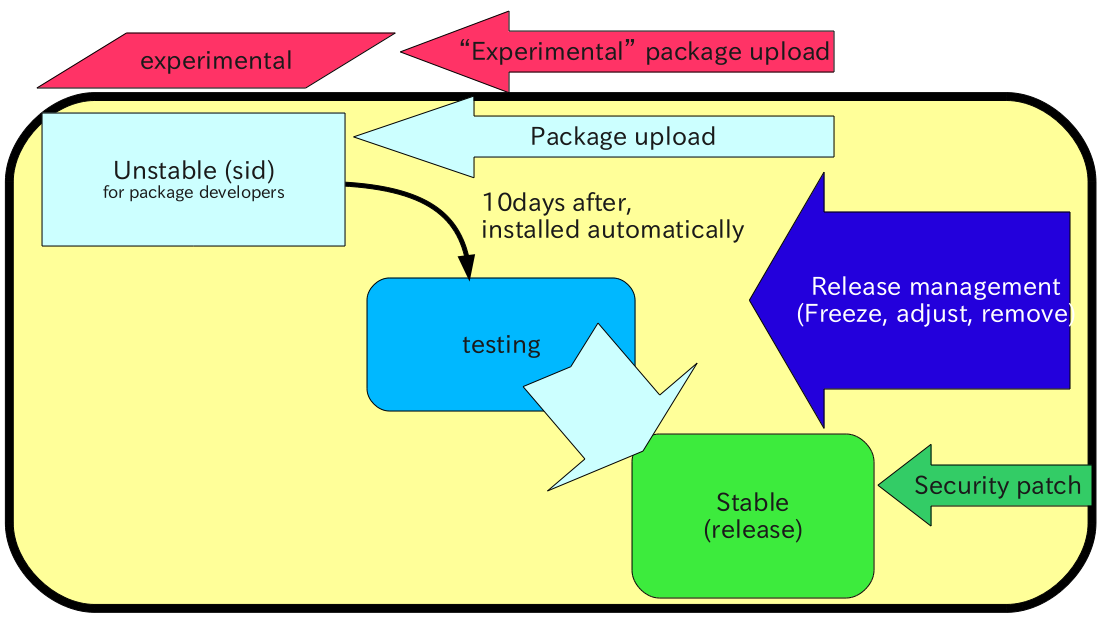
\includegraphics[width=1.05\textwidth]{%
%      ./image201007/201007-debian-development-cycle.png}
%\end{figure}

\subsection{新しい魅力的なソフトウェア}

unstable には私たちをわくわくされるようなソフトウェアが毎日ようにインストールされていく。

\subsubsection{例(1) ibuz-mozc}
\index{ibus-mozc}

open-source project originates from \textbf{Google Japanese Input}.

\begin{itemize}
\item ITP: Bug\#581158

\begin{itemize}
\item もうすぐ unstable に入るYo!
\footnote{既にunstable に入っていますが、non-free扱いです。}
\end{itemize}
\end{itemize}

%\begin{figure}[h]
%\centering
\includegraphics{./image201007/201007-mozc-icon.png}
%\end{figure}

\subsubsection{例(2) chromium-browser}
\index{chromium-browser}

Chromium is an open-source browser project originates from \textbf{Chrome}.

%\begin{figure}[h]
%\centering
\includegraphics{./image201007/201007-chromium-icon.png}
%\end{figure}

\begin{itemize}
\item unstable なら apt 一発
\end{itemize}

\begin{quote}
\begin{verbatim}
% sudo apt-get install chromium-browser
\end{verbatim}
\end{quote}

\subsection{魅力的な更新}

\begin{itemize}
\item emacs \textbf{23}
\item gnome \textbf{2.30}
\item KDE \textbf{4.4.5}
\item ruby \textbf{1.9.2}
\item python 2.7, python3 \dots{}
\end{itemize}


\subsection{最新の○○が使いたい!}

stable に無いなら unstable を使えば良いじゃない.

\subsection{でも unstable はちょっと怖い!? そんな貴方に}

\begin{enumerate}
\item Debian Backports の紹介
\item apt の「ピン止め」
\end{enumerate}


\subsection{Debian Backports}

\underline{\url{http://backports.debian.org/}}

\begin{itemize}
\item 2010/09 から Debianの正式なサービスになった。
\footnote{\url{http://lists.debian.org/debian-announce/2010/msg00012.html}}
\item testing, unstableのソースを\\
stable 向けに再コンパイルしたパッケージを提供

\begin{itemize}
\item security-update にも対応 (BSA (Backports Security Announcement))

\item 公式な安定版よりも新しいバージョンが使える, かも
\end{itemize}

\item 普段は stable を使っているけれども,
特定のソフトウェアは新しいバージョンを使用したい時にオススメ
\end{itemize}


\subsection{backports を使うなら\dots{}}

\begin{itemize}
\item apt-line に以下を追加
\end{itemize}

\begin{commandline}
deb http://backports.debian.org/debian-backports lenny-backports main contrib non-free
\end{commandline}

\begin{itemize}
\item 更新 \& target を指定して install
\end{itemize}

\begin{commandline}
% sudo apt-get update
% sudo apt-get install emacs23 -t lenny-backports
\end{commandline}





\begin{itemize}
\item apt-get upgrade すると

\begin{itemize}
\item lenny-backports のパッケージに upgrade される
\end{itemize}
\item それが嫌なら \textbf{apt のピン止め} を行なうべし
\end{itemize}

\subsection{apt のピン止め}


\begin{itemize}
\item 特定のパッケージ/リリースに対して \textbf{優先度} を設定
\item 優先度に応じて, apt がパッケージを処理する.

\begin{itemize}
\item インストール対象にしない
\item 明示的に指定すればインストール可能\\
アップグレードの対象にはならない
\item ダウングレードしてでも, そのリリースを install する\dots{}などなど
\begin{center}
\end{center}
\end{itemize}
\end{itemize}






\subsection{apt pin の優先度}

\begin{tabular}{ll}
優先度 & 意味 \\
\hline
0 & install しない \\
1--99 & 指定すれば install 可能 \\
 & upgrade の対象にはならない \\
100 & 現在 install されているパッケージ \\
(500) & 現在 install されていないパッケージ \\
(989) & apt-pin の default \\
990 & apt-get の target-release が指定されている場合 \\
1000 以上 & ダウングレードしてもそのパッケージを install \\
\end{tabular}



\subsection{backports 用の pin止めの例}


/etc/apt/preferences に以下の用に書くと?


\begin{commandline}
Package: *
Pin: release a=lenny-backports
Pin-Priority: 99
\end{commandline}

\begin{itemize}
\item release が lenny-backports の
\item 全てのパッケージ (*) を
\item 優先度 99 にピン止め

\begin{itemize}
\item 明示的に指定すればインストール可能
\item アップグレードの対象にはしない
\end{itemize}
\end{itemize}







\begin{itemize}
\item さらに pin 止めするとapt-line に testing/unstable があっても安心
\end{itemize}

\begin{commandline}
Package: *
Pin: release a=lenny-backports
Pin-Priority: 99

Package: *
Pin: release a=testing
Pin-Priority: 98

Package: *
Pin: release a=unstable
Pin-Priority: 97
\end{commandline}






%\newpage

\subsection{野良 backports の作り方}

欲しいパッケージが \\backports に無いよ?
%backports に無いならunstable を使えば良いじゃない.
野良 backports を作ろう!


\begin{itemize}
\item 材料

\begin{enumerate}
\item 安定版の動いているマシン
\item testing/unstable の \textbf{ソースパッケージ}
\end{enumerate}

\item レシピ

\begin{enumerate}
\item apt の pin 止めをする
\item apt-get source \textbf{パッケージ名} -t testing(unstable)
\item 依存するパッケージを install してパッケージ作成

\begin{itemize}
\item パッケージが古くて依存関係が満たせない\\
→ 2. に戻ってくりかえし
\end{itemize}
\end{enumerate}
\end{itemize}

% debianmeetingresume201006-kansai.tex
\dancersection{dh {\normalsize $\sim$source format 3.0, the magic debhelper rules$\sim$}}{佐々木洋平}

\index{quilt}
\index{source format 3.0}

次期安定版 6.0(squeeze)での RELEASE GOALS の一つに「new source package format support」があります\footnote{\url{http://release.debian.org/squeeze/goals.txt}}。
ここでの「new source package format」が {\bf source format 3.0} です。
\vspace{1em}

{\tt debhelper} は deb パッケージの構築を補助する様々なツール群です%
\footnote{%
deb パッケージそのものは {\tt debhelper} 無しでも作成できますが、
普通は {\tt debhelper} を使います。}。
多くのパッケージでは {\tt debhelper} の呼び出しはテンプレ化されているので
共通している {\tt debhelper} の呼び出しを隠蔽し
パッケージ作成のルール(debian/rules)を簡単にするのが
{\tt dh}(コマンド)と {\tt CDBS}(Makefile のルールセット)です。
\vspace{1em}

ここでは source format 3.0, dh, CDBS についてお話しします。
ちなみに、
告知タイトルに「深追い」とか「CDBS 2.0」とかいう文字列があった気がしますが
気にしないで下さい。

\subsection{source format 1.0 $\to$ 3.0 }

\subsubsection{1.0 の問題点}

source format 3.0 の前に、
これまでの source format 1.0 について簡単に復習しましょう。debian のソースパッケージは主に以下の構成物からなります:
\begin{quote}
    \begin{screen}
        \begin{description}
              \item[.orig.tar.gz]  \\
            オリジナルのソース一式
              \item[.dsc] \\
            パッケージの情報(パッケージの説明、メンテナ、ファイルのハッシュなど)
              \item[.diff.gz] \\
            バイナリパッケージをビルドするための変更点。
            Debian 固有のパッケージの場合には存在しない。
        \end{description}
    \end{screen}
\end{quote}

さて, このソースフォーマットの構成には, 以下の問題点があります:
\begin{enumerate}
      \item アーカイブの圧縮形式として .gz  しか使えない。
      \item upstream のソースが複数のアーカイブから構成される場合が面倒。
      \item パッケージメンテナの作成したパッチが全部単一のファイルにま
    とめられており、混然としている。
      \item diff で表現されるので(画像などの)バイナリが置きにくい。
\end{enumerate}

source format 1.0 の場合、これらの問題点は, だいたい以下の様に解決していました:
\begin{quote}
    \begin{description}
          \item[1. アーカイブの圧縮形式として .gz しか使えない。]  \\
        % 
        例えば upstream が bzip2 で配布されている場合でも gzip で圧縮しなお
        す、 もしくは tarball in tarball \footnote{%
          .orig.tar.gz を展開するとディレクトリ内にupstream の bzip2 が配置
          される。ビルドする際に tar を展開してからビルドする} などの形式に
        する、などです。
        % 
        後述の CDBS を使用する場合には tarball in tarball 用のルールとして
        {\tt tarball.mk} が用意されています。
        % 
           \item[%
        2. upstream のソースが複数のアーカイブから構成される場合が面倒。] \\
        % 
        前述の tarball in tarball で対応しています。
        % 
          \item[3. パッケージメンテナの作成したパッチが全部単一の patch に。]
         \\
        % 
        {\tt diff.gz} は {\tt debian} 以下のファイルが{\bf 全て}単一の
        ファイルになっています。{\tt debian/control} や 
        {\tt debian/rules} だけではなく、upstream のソースへのパッチも全て
        一つのファイルになっています。
        % 
        そこで、upstream のソースへのパッチは {\tt debian/patches} 以下に
        意味のある単位で分割して配置し、パッケージ作成の際に
        パッチの apply/unapply を行なうことにしています。
        % 
        このためのツールとしては{\tt dpatch} や
        {\tt quilt}
        \footnote{%
          こう書くと語弊があるかもしれませんが、
          {\tt quilt}は Debian 固有のツール{\bf ではありません}。
        %
          一方で dpatch は
          「patch maintenance system for Debian source packages」と
          あるように Debian 固有のツールです。
        }
        があります。
        % 
        また、CDBS にはパッチの apply/unapply をするためのルールとして
        {\tt patchsys-quilt.mk, dpatch.mk, simple-patchsys.mk}
        が用意されていますし、
        dh には{\tt --with quilt} というオプションが用意されています。
        % 
        ちなみに、
        各パッチの先頭にその意図を記述するタグを追加しておくことが推奨
        されています
        \footnote{\url{http://dep.debian.net/deps/dep3/} 
          面倒なので佐々木はサボリがちです。すいません。}。
        % 
          \item[4. diff で表現されるので(画像などの)バイナリが置きにくい。] \\
        uuencode/uudecode で diff が取れる形式にしておくなどして
         対応します。
    \end{description}
\end{quote}

というわけで、これまでの source format でも問題点について対応はできます。
しかしながら、
こういった特殊な操作を行なうことなく
問題点を解決するための新たなフォーマットとして、新たに
{\tt 3.0 (quilt)} と {\tt 3.0 (native)} が制定されました%
\footnote{%
  \url{http://wiki.debian.org/Projects/DebSrc3.0} 
  ちなみに 2.0 はどういう状況知りません. だれかご存知ですか?
}。

\subsubsection{3.0(quilt) と 3.0(native)}

{\tt 3.0 (quilt)} は以下のファイル群で構成されます:
\begin{quote}
    \begin{screen}
        \begin{description}
              \item[{\tt .orig.tar}.{\it ext}]  \\
            upstream のソース。複数のソースからなる場合には基本となるソースに
            この名前をつける。{\it ext} は圧縮の拡張子であり、
            gz, bz2, lzma, xz が使用可能。
            % 
              \item[{\tt .orig}{\it -component1}{\tt .tar.}{\it ext}] \\
            upstream が複数のソースから構成される場合に作成する。
            % 
            {\it -componet} はソースの名前に対応してメンテナが適宜名付ける。
              \item[{\tt .debian.tar.}{\it ext}] \\
            {\tt debian} ディレクトリの中身。
            {\it ext} は圧縮の拡張子であり、
            gz, bz2, lzma, xz が使用可能。
            %
            1.0 の {\tt diff.gz} から
            {\tt .tar.}{\it ext} になり、全てが混在した単一のパッチでは
            なくなった。
            % 
              \item[{\tt .dsc}]  \\
          パッケージに関する情報。
        \end{description}
    \end{screen}
\end{quote}
また {\tt 3.0 (native)} は 1.0 での Debian 固有パッケージに対応しており、
{\tt .orig.tar.}{\it ext} と {\tt .dch} ファイルからなります。

%
これらの変更により 1.0 での問題点は以下の様に解決されました。
\begin{enumerate}
      \item アーカイブの圧縮形式として .gz しか使えない。\\
    $\to$ .gzip, bzip2, lzma, xz を使用できるようになりました。
    %
      \item upstream のソースが複数のアーカイブから構成される場合が面倒。\\
    $\to$ {\tt .orig}{\it -component}{\tt .tar}{\it .ext} により
    複数のソースを使用できるようになりました。
    %
    これら{\tt .orig}{\it -component}{\tt .tar}{\it .ext} は
    ソースの展開時に {\tt compnent} というサブディレクトリに展開されます。
      \item パッケージメンテナの作成したパッチが全部単一のファイルに。
      \item diff で表現されるので(画像などの)バイナリが置きにくい。\\
    $\to$ {\tt .diff.gz} から {\tt .debian.tar.}{\it ext} になったので
    全てが混然となった状態は解消されており、バイナリも含めることができます。
    また、 {\tt debian/patches} に存在するパッチはソースパッケージの展開時に
    自動的に適用されるようになりました(これについては後述)。
\end{enumerate}

現在では、日々巨大化しつつある  Debian アーカイブのサイズを抑制するために
新規パッケージについては {\tt gzip} よりも {\tt xz} による圧縮が推奨されています。

\subsubsection{3.0 への移行}

さて source format 3.0 に以降するにはどうすれば良いでしょうか? 
複雑なパッケージでないならば、
\begin{commandline}
    % mkdir debian/source
    % echo '3.0 (quilt)' > debian/source/format
    % dch 'Switch to dpkg-source 3.0 (quilt) format' 
\end{commandline}
だけでです. 

これまでの diff.gz に upstream へのパッチが含まれている場合には、
先ずパッチを(意味のある単位に)分割し、
quilt で管理できるようにしておきましょう。
そうしない場合には分割されていないパッチは
{\tt debian/patches/debian-changes-<version>} という
patch にまとめられてしまいます\footnote{というわけです $>$ lurdan}。
また、
更新の度に{\tt debian-changes-<version>} というパッチが生成されてしまいます。
%
また quilt は -p1 のパッチしか扱えませんので rules 内で明示的に patch
-p0 とか patch -p2 としている場合や、 CDBS の simple-patchsys.mk を使用
している場合には -p1 で適用できるようにパッチを変更しておきます。

最後に debian/rules でのパッチに関する rules を消しておくことが推奨され
ています。dpkg ($>$=1.15.5.4) では dpkg-source によってソースを展開する
際にdebian/patches 以下のパッチが自動的に適用されることは既に述べました。
古い buildd、とくに lenny 向けの buildd ではソースを buildd chrootの外
で展開することがあるため, dpkg-source の段階でソースにパッチが適用され
ていない場合には不具合が生じます。
%
パッチを更新した場合には debuild を実行する前にパッチを全て適用しておき
ます。こうして debuild を実行すると、3.0 形式のソースパッケージが生成さ
れます。

ちなみに lenny の dpkg は既に 3.0 に対応しています。これ
はlenny で squeeze のソースパッケージを使用する場合(backports 等)に問題
にならないようにするためです。 また、現在は {\tt debian/source/format}
で source format のバージョンを指定していますが、将来的には全て新しい
source format へ移行される予定です。
\begin{center}
    {\tt ではお手元のソースを 3.0 へ移行してみましょう}    
\end{center}

\subsection{debian/rules の書き方}

CDBS, dh 以前の debhelper コマンド群を使用した {\tt debian/rules} は
一番簡単な場合でも、
例えば以下の様になります
\footnote{lenny で GNU Hello のパッケージを作成した場合です。
ページに収めるために先頭のコメントを削っています。}。
\begin{commandline}
#!/usr/bin/make -f
# -*- makefile -*-
# Sample debian/rules that uses debhelper.
# - snip -

# Uncomment this to turn on verbose mode.
#export DH_VERBOSE=1
 
# These are used for cross-compiling and for saving the configure script
# from having to guess our platform (since we know it already)
DEB_HOST_GNU_TYPE   ?= $(shell dpkg-architecture -qDEB_HOST_GNU_TYPE)
DEB_BUILD_GNU_TYPE  ?= $(shell dpkg-architecture -qDEB_BUILD_GNU_TYPE)
ifneq ($(DEB_HOST_GNU_TYPE),$(DEB_BUILD_GNU_TYPE))
CROSS= --build $(DEB_BUILD_GNU_TYPE) --host $(DEB_HOST_GNU_TYPE)
else
CROSS= --build $(DEB_BUILD_GNU_TYPE)
endif
config.status: configure
        dh_testdir
        # Add here commands to configure the package.
ifneq "$(wildcard /usr/share/misc/config.sub)'' "
        cp -f /usr/share/misc/config.sub config.sub
endif
ifneq ``$(wildcard /usr/share/misc/config.guess)" ""
        cp -f /usr/share/misc/config.guess config.guess
endif
        ./configure $(CROSS) --prefix=/usr --mandir=\$${prefix}/share/man --info
dir=\$${prefix}/share/info CFLAGS=''$(CFLAGS)" LDFLAGS="-Wl,-z,defs"


build: build-stamp

build-stamp:  config.status
        dh_testdir

        # Add here commands to compile the package.
        $(MAKE)
        #docbook-to-man debian/hello.sgml > hello.1

        touch $@

clean:
        dh_testdir
        dh_testroot
        rm -f build-stamp

        # Add here commands to clean up after the build process.
        [ ! -f Makefile ] || $(MAKE) distclean
        rm -f config.sub config.guess

        dh_clean

install: build
        dh_testdir
        dh_testroot
        dh_clean -k
        dh_installdirs

        # Add here commands to install the package into debian/hello.
        $(MAKE) DESTDIR=$(CURDIR)/debian/hello install

# Build architecture-independent files here.
binary-indep: build install
# We have nothing to do by default.

# Build architecture-dependent files here.
binary-arch: build install
        dh_testdir
        dh_testroot
        dh_installchangelogs ChangeLog
        dh_installdocs
        dh_installexamples
#       dh_install
#       dh_installmenu
#       dh_installdebconf
#       dh_installlogrotate
#       dh_installemacsen
#       dh_installpam
#       dh_installmime
#       dh_python
#       dh_installinit
#       dh_installcron
#       dh_installinfo
        dh_installman
        dh_link
        dh_strip
        dh_compress
        dh_fixperms
#       dh_perl
#       dh_makeshlibs
        dh_installdeb
        dh_shlibdeps
        dh_gencontrol
        dh_md5sums
        dh_builddeb

binary: binary-indep binary-arch
.PHONY: build clean binary-indep binary-arch binary install    
\end{commandline}
configure、make、 make install 以外にも随所に dh\_ から始まるコマンドが
呼び出されています。
%
この dh\_ から始まるコマンドが debhelper コマンド群です。
%
幾つかの例外を除いて dh\_* は適切なタイミングで呼び出すだけですので、
この呼び出しを隠蔽するだけで debian/rules は随分すっきりします。
CDBS, dh は異なる手法で dh\_* の呼び出しの隠蔽とルールセットの追加を
行なっています。

\subsubsection{CDBS}

CDBS については以前お話しました(2008年6月, 第 18 回関西Debian勉強会%
\footnote{\url{http://tokyodebian.alioth.debian.org/pdf/debianmeetingresume200810-kansai.pdf}})。{\tt debian/ruls} は Makefile ですので
\begin{itemize}
      \item Makefile の target を細分化。
      \item ソフトウェアやパッケージの状況に応じて、
    呼び出す target を class としてまとめる。
\end{itemize}
としています。

CDBS を利用した場合のビルドターゲットの流れについては例えば
杉浦さんの Web に良い絵が公開されています
(これは buildcore.mk + debhelper.mk を用いた場合です)。
\begin{figure}[h]
    \centering
    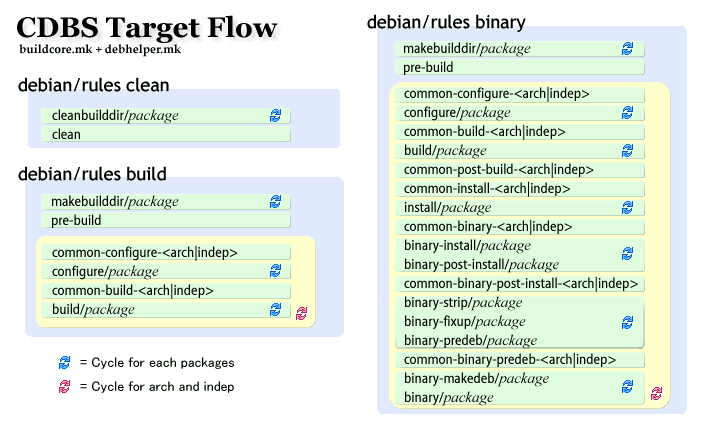
\includegraphics[width=0.7\textwidth]{./image201006/cdbs-targets.png}
    \caption{%
      CDBS Target flow:
      \url{http://sugi.nemui.org/doc/cdbs/cdbs-targets.png}}
    \label{fig:CDBSTargetFlow}
\end{figure}

CDBS を使った場合、先程の GNU Hello のルールは
\begin{commandline}
#!/usr/bin/make -f

include /usr/share/cdbs/1/rules/debhelper.mk
include /usr/share/cdbs/1/class/autotools.mk
\end{commandline}
となります。
以前書きましたが, %
いきなりコレだと今度は何をしているのかわからなくなりますね(笑)。

最初の include が dh\_* の呼び出しを設定する class, 
二つ目の include が autotools を使用するソースからパッケージを作成する場合の
class です。CDBS の詳細については本家のドキュメント\footnote{%
CDBS Documentation: \url{http://cdbs-doc.duckcorp.org/en/cdbs-doc.xhtml}}
が参考になるでしょう。
%
パッケージに付属のドキュメントではソースには実装されていて使えるのに
ドキュメント化されていない便利機能が多いです。
%
こういう場合は「ソース見れば良いじゃん」というのはまあ正論ではあります。%
実際、class のカスタマイズに使用する変数はソース冒頭に定義されてますし...。


\subsubsection{dh - debhelper command sequencer}

CDBS が make の target の細分化$\to$class 化という方向で dh\_* の呼び出
しを隠蔽し、Gnome、KDE といった統合環境や perl、python といった言語用
の class によって rules の作成を容易にしているのに対して、
dh のアプローチは以下の通りです:
\begin{itemize}
      \item debhelper の呼び出しは隠蔽したまま
      \item 
    パッケージ作成に使用するツール(autotools, make, MaikeMaker 等)
    の自動判定を行なう
\end{itemize}


例えば先程の GNU Hello の場合には
となります。
\begin{commandline}
#!/usr/bin/make -f

%:
        dh $@
\end{commandline}
...CDBS よりさらに簡潔になりました(笑)。

さて、これでは CDBS 以上にナニをしているのかわかりませんね。
実は dh コマンドには {\tt --no-act} というオプションが用意されています。
試しに rules を書き換えずに binary ターゲットを --no-act つきで
実行してみましょう。
\begin{commandline}
   uwabami@vmguest-lenny:~/Packages/hello-2.6$ dh binary --no-act
   dh_testdir
   dh_auto_configure
   dh_auto_build
   dh_auto_test
   dh_testroot
   dh_prep
   dh_installdirs
   dh_auto_install
   dh_install
   dh_installdocs
   dh_installchangelogs
   dh_installexamples
   dh_installman
   dh_installcatalogs
   dh_installcron
   dh_installdebconf
   dh_installcatalogs
   dh_installemacsen
   dh_installifupdown
   dh_installinfo
   dh_installinit
   dh_installmenu
   dh_installmime
   dh_installmodules
   dh_installlogcheck
   dh_installlogrotate
   dh_installpam
   dh_installppp
   dh_installudev
   dh_installwm
   dh_installxfonts
   dh_lintian
   dh_desktop
   dh_gconf
   dh_icons
   dh_perl
   dh_pysupport
   dh_scrollkeeper
   dh_usrlocal
   dh_link
   dh_compress
   dh_fixperms
   dh_strip
   dh_makeshlibs
   dh_shlibdeps
   dh_installdeb
   dh_gencontrol
   dh_md5sums
   dh_builddeb
\end{commandline}
と出力されます。CDBS と違って、ビルド時の流れを見る事ができます。
dh コマンドの肝は
\begin{center}
    {\tt dh\_auto\_}
\end{center}
で始まる 5 つのコマンドです。

何も設定しない場合には dh\_auto\_configure がパッケージの
ビルド時に使用するツールを判定します。この判定結果に基づき
auto\_build, auto\_test, auto\_install が実行されます。
自動判定結果は基本的に良くある GNU な設定になっており、
例えば configure 時の --prefix=/usr とか install 時の DESTDIRなどは
GNU のパッケージ用に設定されています(なので GNU Hello は設定が不要です)。

注意して欲しいのは configure や configure.ac をパースしているわけではないので
dh\_auto\_* は変数を自動設定をしているわけではない、という事です。
configure に対して Debian パッケージ用のフラグを適用したり、環境変数を追加
する場合には、適宜変数を設定してやったりする必要があります。
%
また、ソフトウェアによっては
ビルド時に configure, make, make install 以外の操作をする必要があったりします。
このための機能が dh の {\tt override} と {\tt before, after} です。

\subsubsection{実践! the magic debhelper rules}

例えば GNU Hello の configure オプションには
{\tt --with-gnu-ld} や {\tt --disable-nls} といったオプションがあります。
これらを configure 時に指定したい、と思ったらどうしたら良いでしょう?
この場合には dh\_auto\_configure の呼び出し時にオプションを与えるようにします。
例えば lenny の場合には {\tt --before, --after} を使用します。
\begin{commandline}
#!/usr/bin/make -f

%:
        dh $@

build: build-stamp
build-stamp:
        dh build --before configure
        dh_auto_configure -- --with-gnu-ld --disable-nls
        dh build --after configure
        touch build-stamp
\end{commandline}
squeeze/sid の dh には {\tt override} という機能が追加されており、
記述がさらに簡単になります%
\footnote{override は debhelper ($>$= 7.0.50) 以降の機能です。}。
\begin{commandline}
#!/usr/bin/make -f

%:
        dh $@

overide_dh_auto_configure:
        dh_auto_configure -- --with-gnu-ld --disable-nls
\end{commandline}
squeeze/sid 版の override の方が直感的にわかりやすいですね。 
また、squeeze/sid の dh コマンドは --no-act の際に override 
を表示してくれます。
\begin{commandline}
uwabami@vmguest-sid:~/Packages/hello-2.6$ dh binary --no-act
  dh_testdir
  debian/rules override_dh_auto_configure
  dh_auto_build
  dh_auto_test
  ...
\end{commandline}
override の詳細までは表示されませんが override されていること、
及び呼び出しの順番が参照できます\footnote{%
西山さんの DEB\_UPDATE\_RCD\_PARAMS の場合は
dh\_installinit を override すれば良いと思います.}。

以下では squeeze/sid の dh コマンドについて解説します。
残念ながら lenny の debhelper は若干古いですので、
sqeeze/sid の debhelper を導入しましょう。
%
dh コマンドの使い方については
Debconf9 での Joey Hess 御大による debhelper のプレゼン資料
\footnote{%
\url{http://joey.kitenet.net/talks/debhelper/debhelper-slides.pdf}}
が今の所一番まとまっている気がします。
御大のプレゼン資料に掲載されている
dh コマンドを利用した rules の例を以下に示します。
\begin{enumerate}
      \item 自動判定結果とは別のビルドツールを使用
    \begin{commandline}
#!/usr/bin/make -f

%:
    dh $@ --buildsystem perl_build
    \end{commandline}
      \item upstream のソースファイルがサブディレクトリ src にあり
    ビルドを make -C で別ディレクトリ(ここでは build)で実行
    \begin{commandline}
#!/usr/bin/make -f

%:
    dh $@ --sourcedirectory=src \
          --builddirectory=build
    \end{commandline}
      \item パッチ当てに quilt を使用して、
    configure にフラッグを指定、changelog として changelog.html
    を収録
    \begin{commandline}
#!/usr/bin/make -f

%:
    dh $@ --with quilt \
          --builddirectory obj \
          --sourcedirectory source 

override_dh_auto_configure:
    autoconf
    dh_auto_configure -- --with-sdl CC=/usr/bin/gcc-4.1

override_dh_installchangelogs:
    dh_installchangelos changelog.html
    \end{commandline}
 \end{enumerate}
などなど。

\subsection{debhelper vs CDBS vs dh }

Joey Hess 御大のプレゼン資料では
\begin{itemize}
      \item debhelper で設定可能な項目は 138
      \item CDBS で設定可能な項目は 138 + 153
      \item dh で設定可能な項目は 138 + 12
\end{itemize}
となっています。

御大は「私が比較するのは unfair だ」とおっしゃってますが、
rules の可読性/可変性は dh の方が圧倒的に優れていると思います。
特に、dh の一番嬉しい所は
--no-act による work frow が把握しやすいことでしょう。
また、Build-Depends が減る、というのは一つの利点かもしれません。

一方、CDBS は work flow は把握しにくいですけれど対応している
ビルドツールが多い事があげられます。
CDBS 本体には Make, SCons(Make の代替品), 
Perl, Python, Cmake, Ant,  Qmake, Gnome, KDE の class がありますし、
本体には収録されていませんが pkg-kde-tools, pkg-ruby-tools が提供されています。
これらの class を使用することで rules は共通化され非常に簡潔に記述できます。
dh の場合, 現時点で対応しているビルドツールは
\begin{commandline}
uwabami@vmguest-sid$ dh_auto_build --list
autoconf             GNU Autoconf (configure)
perl_makemaker       Perl ExtUtils::MakeMaker (Makefile.PL)
makefile             simple Makefile
python_distutils     Python Distutils (setup.py)
perl_build           Perl Module::Build (Build.PL)
cmake                CMake (CMakeLists.txt)
ant                  Ant (build.xml)
qmake                qmake (*.pro)
\end{commandline}
といった所です。


\begin{center}
    {\tt ではお手元のソースを CDBS or dh へ移行してみましょう. \\
    既に CDBS を使用している場合には dh で書きかえて見て下さい。}
\end{center}

最後に妄想など。
%
現在手元で dh\_ruby 関連を作成中です。
setup.rb, extconf.rb ができれば多分 CDBS とは別の選択肢になるだろう, と
思っています(あとは rake 用の build 拡張ができれば dh\_make\_gems の完成です)。
これについては...時間と紙面の都合で今日は載せられません。そのうち勉強会で
お話しします。
というわけで、「深追い」はタイトルに偽りアリ、ですね。すみません...{\tt Orz}

%debianmeetingresume201008-kansai.tex
\dancersection{Emdebian について}{たなかとしひさ}

\index{emdebian}

\subsection{前書き}

この資料は、筆者が Emdebian を使う上で勉強した事を記載しています。まだま
だ、完全に理解したわけではなく、部分部分でしかEmdebianを使えていませんが、
中間報告と言う事でご容赦ください。

\subsection{Emdebian って?}

Emdebian (Embedded Debian)は、Debian GNU/Linuxを元に、組込み機器用途に最
適化していくプロジェクトです。

Debian GNU/Linux は、まず Debian自身がマルチアーキテクチャ(勉強会課題1)に
対応しています。また、どのベンダーからも独立しており、Debian 社会契約、お
よび膨大な利用可能ソフトウェアは様々な選択肢を可能にしますが、デスクトッ
プ環境(大きなハードディスクとメモリ)に向けられています。

`Embedded Debian`は、Debian のメリットを活かしつつ、組込み機器の様な小さ
いシステム向けに Debian を軽量にするものです。

(上記は、\url{http://www.emdebian.org/}から意訳したものです)

\subsubsection{勉強会課題1: Debian が動作する CPU、ターゲット機器}

\url{http://www.jp.debian.org/ports/}から、Debian の移植版に関する情報が
得られます。

\begin{itemize}
 
 \item Intel x86 / IA-32 (i386) - 1番身近で使われていますね。 
 \item (Motorola 68k (m68k)) - Etch 以降のリリースには含まれていません。
 \item  Sun SPARC (sparc)

 \item  Alpha (alpha)
 \item  Motorola/IBM PowerPC (powerpc)
 \item  ARM (arm および armel) - 今回取り上げる CPU です。
 \item  MIPS CPUs (mipsとmipsel)
 \item  HP PA-RISC (hppa)
 \item  IA-64 (ia64)
 \item  S/390 (s390)
 \item  AMD64 (amd64)
\end{itemize}
また、移植中のターゲットとして、以下のものがあります。
\begin{itemize}
 \item ARM のハードウェアfloat対応 (armhf) 
 \item Atmel 社 AVR32 向け (avr32)
 \item powerpc + SPE 命令 向け (powerpcspe)
 \item Renesas Electronics社 sh4 向け
 \item Sparc 64bit 向け (sparc64)
\end{itemize}

Debianは、カーネルにLinuxカーネルを使いますが、Debian GNU/kFreeBSDの様に、
カーネルにFreeBSDのカーネルを使うものもあります。

\subsubsection{勉強会課題2: 皆さん、上記の内、使った事のあるアーキテクチャを教えてください。}

なお、Emdebian は、下記のアーキテクチャが利用可能です。

i386、amd64、powerpc、armel、mips、mipsel, sh4

\subsection{Emdebian は何を作っているか(何を作ろうとしているか)。}

\begin{description}
% emdebian はクロスコンパイラだけ。
% \item[Toolchains]\mbox{}\\ 
%           gccを初めとした、ビルド済みの開発環境です。
 \item[Smaller packages]\mbox{}\\
  \begin{description}
   \item[Emdebian Grip - binary-compatible with Debian](今回お話しするものはこれです)

              これは、Debian からインストールできる(要するにdebootstrap でインストールできる)ものです。
   \item[Emdebian Crush - cross-built, customised Emdebian installations without perl]\mbox{}\\
              Web ページによると、Busybox をベースにした root filesystem
              との事です。

              Busybox であるため、Debian そのものと構成が変わっている事が
              考えられますが、Emdebian Grip と比べると、もっと容量は小さ
              いと考えています。
  \end{description}

 \item[Cross building tools]\mbox{}\\
            その名の通り、クロス開発ツールです。

            「クロス開発」とは、例えばパソコン(i386)上で、ARM のバイナリ
            を生成する様な、ホスト(コンパイル)環境とターゲット(実行)環境
            のCPUやOSが異なる場合の開発を言います。

            組込み機器は、その殆どがクロス開発で作ります。

            他方、ホスト環境とターゲット環境が同じ、単純に言えば、i386上
            で、i386上で動くソフトウェアを開発する場合は、「セルフ開発」
            と言います。

            Emdebianは、Debian正規のものと同期しながら、クロス開発環境に
            焦点を当てています。i386と amd64アーキテクチャ上で、arm,
            ia64, m68k, mips, mipsel, powerpc, sparcのビルドが可能です。
 \item[Root filesystem generation is based on multistrap package.]\mbox{}\\
            multistrapは、Emdebianでroot filesystemを作るうえでのメインと
            なるツールです。

            (ごめんなさい、multistrap はまだ筆者が十分に勉強できていませ
            ん…)
\end{description}

Emdebian自身、まだ作業中のものが多く、協力者を募集しています。

\url{http://www.emdebian.org/emdebian/helpout.php} このページに、
EmdebianのToDo(バグリスト)があります。

\subsection{なぜ、「組込み Linux」なのか?(なぜ「組込み Debian」なのか?)}

理由は人それぞれですが、筆者自身が強く感じるのは、組込みLinuxは、プログラ
ムの動作確認が容易になり、ソフトウェアの品質を確保しやすくなると言う事で
す。

例えば、日本の組込み機器で使うOSにはITRONを使う事が多いです。海外だと
VxWorksを使う事が多いです。ITRONを使った開発の場合、ITRONのシステムコー
ルは、PCではシミュレータ(あるいはエミュレータ)を使わない限り、動きを含め
た動作確認は出来ません。

そのため、JTAG等のデバッガを使って、実機にプログラムを焼きこんでデバッグ
する事が殆どです。

組込みLinuxの場合、i386 版 Linux で、ある程度動きも含めたデバッグも可能に
なります。

ARM版Linux向けのプログラムを作るとして、一々ARM版プログラムをビルドして
ARM CPUなターゲットボードに転送するよりも、i386版Linuxで粗方デバッグして
おき、ターゲット環境では実際のターゲットならではのデバッグに注力すれば、
デバッグ時間を削減できます。デバッグ時間を削減できると言う事は、ソフトウェ
アテスト等の時間を増やす事が出来ると言う事であり、ソフトウェアの品質向上
に繋げることが出来ます。

確かに、ターゲット機器上で全て動作確認をすべきですが、ターゲット機器上で
トレースデバッグをするよりも、ホスト環境上で基本的なデバッグができるのは
魅力で効果的です。

Linuxは、無料で使用できますが、筆者は、有料/無料とは別に、ソフトウェアの
品質を確保しやすいという点で、組込みLinuxは他のOSよりも優位性があると考え
ています。

さらに、組込み Debianは、PC等で得たDebianの知識を、組込み機器にも活かす事
が出来ます。ソフトウェアの不具合のいくつかは、不慣れな(未知な)環境下であっ
た事に起因する不具合があります。普段から使い慣れているOS(Debian)が使える
事も、ソフトウェアの品質を確保する上で重要なのです。

最後に、Debianはベンダー独立、別の言い方をすると…倒産する事がないです :-)。

「Linux企業」は、自主独立で歩き続けているベンダーもあれば、吸収合併、ある
いは部門売却などで看板が変わり、契約が変わる場合があります。

「Linux企業」と契約する側にしてみれば、Linux企業と契約したものの、ある日
部門売却等で契約先が変わり、再度新規契約からやり直し…となるのは手間です。
もしそこで費用面から話をしなければならないとすると、Linuxを使うこと自身に
消極的になります。

Debian は、その様な事はありませんので、安心して使い続けることが出来ます。

\subsection{Emdebian Grip を試してみる。}

Emdebian Grip を、MINI2440 にインストールしてみました。

厳密に言うと… rootfsはEmdebian Gripですが、LinuxカーネルはEmdebianそのも
のではありません。すみません。これも引き続きの勉強課題とさせてください。

写真は、MINI2440にEmdebian Gripをインストールして、iceweaselで
OpenStreetMapのページを参照したものです。ARM上でWebブラウザが普通に使えま
す(但し遅いです)。rootfsはSDカードを使っています。

\begin{center}
 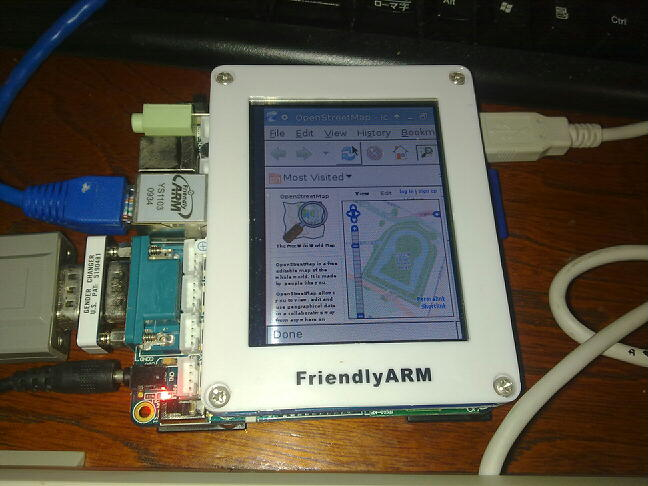
\includegraphics[width=0.5\hsize]{image201008/emdebian.jpg}
\end{center}

MINI2440の詳しい情報は、\url{http://www.friendlyarm.net/products/mini2440}を参照してください。

\subsubsection{必要なもの}

まず、MINI2440のNANDフラッシュROMのバックアップを取るには、残念ながら
MS-Windows上で動くソフトウェア(DNW)が必要です。筆者は、NANDフラッシュROM
のバックアップと、ブートローダ(U-Boot)書き込みに(不本意ですが)MS-Windows
を使いました。(後すみません、TeraTermも使いました)

他に必要なものを以下に記します。
\begin{itemize}
 \item MINI2440本体
 \item i386(amd64)な Debian
 \item ネットワーク
 \item シリアルケーブル(クロスケーブル)
 \item SDカード(1GByte~2GByte)(Debian PCからアクセスするので、カードアダプタも必要)
\end{itemize}

\subsubsection{MINI2440のEmdebian化}

\subsubsubsection{MINI2440 NAND フラッシュのバックアップ(必要なら)}

MINI2440は、購入した状態ではNANDフラッシュROM にQt/Embeddedがインストール
されていますので、もし必要ならばバックアップしてください。

\subsubsubsection{Emdebian Grip rootfs の取得}

\url{http://code.google.com/p/mini2440/wiki/Emdebian}を参考に、Emdebian
Gripのrootfsを取得します。ここではdebootstrapを使いますので、適宜
apt-get等でインストールしておいてください。

Emdebian Grip rootfs は、上記URLに記載している手順で進められます…が、こ
のURLでは、Emdebian Grip向けLinuxカーネルビルドに関する事が無いので、
Emdebian Grip向けのLinuxカーネルをビルドする必要があります。

\subsubsubsection{MINI2440(Emdebian Grip)向けLinuxカーネルのビルド}

MINI2440(Emdebian Grip)向けLinuxカーネルをビルドするには、最低限下記のも
のが必要です。

\begin{enumerate}
 \item Toolchain(gcc)
 \item (MINI2440に対応した)Linux カーネルソース
\end{enumerate}

できれば、それこそEmdebianで一撃に…と思ったのですが、筆者は
\url{http://code.google.com/p/mini2440/downloads/list}から得られる
mini2440-bootstrap-v2.shと言うシェルスクリプトを改造して使いました。

このシェルスクリプト(mini2440-bootstrap-v2.sh)は、開発環境(CodeSourcery)や
MINI2440向けLinuxカーネルを自動的にダウンロードしてビルドします。

なお、mini2440-bootstrap-v2.shは、Debian上でも使えますが、U-Bootのソース
コードはダウンロードしますがビルドはしないので、下記の様に修正して使いま
す。

\begin{commandline}
 tosihisa@lavie:~/Downloads$ diff -ca mini2440-bootstrap-v2.sh mini2440-bootstrap-v2.sh.change
 *** mini2440-bootstrap-v2.sh    2010-08-17 17:19:45.000000000 +0900
 --- mini2440-bootstrap-v2.sh.change     2010-08-17 17:19:13.000000000 +0900
 ***************
 *** 72,78 ****
  # compile bits
  cd ${DEST}/uboot/mini2440
  make mini2440_config
 ! # make clean all

  cd ${DEST}/kernel/mini2440

 --- 72,78 ----
  # compile bits
  cd ${DEST}/uboot/mini2440
  make mini2440_config
 ! make clean all

  cd ${DEST}/kernel/mini2440

 tosihisa@lavie:~/Downloads$
\end{commandline}

\subsubsubsection{U-BootをMINI2440にインストールする。}

MINI2440は、Superviviと言うブートローダがNORフラッシュ側にありますが、
NANDフラッシュ側にU-Bootをインストールします。

U-Boot(the Universal Boot Loader)は、Linux カーネルだけでなく、ELF形式で
あればロードできるブートローダです。また、ブートローダとしての機能だけで
はなく、メモリ操作が可能なので、デバッグツールとしても利用できます。

U-Bootは、\url{http://www.friendlyarm.net/downloads}から入手できるビルド
済みのバイナリ(u-boot\_20100701.zip)を使いました。

\subsubsubsection{Emdebian Grip を起動…}

rootfsを作り、Linux カーネルをビルドできたら、それらをSDカードにコピーし
ます。
U-BootをMINI2440に焼きこめたら、Linuxを起動します。

debootstrap 直後のSDカードで起動した場合、完全にはインストールが完了して
いませんので、U-Bootのブートパラメータに'init=/bin/sh'を与えて、シェルを
起動させるようにします。

その後、(MINI2440で起動したEmdebianで)シェルが起動したら、ネットワークが
DHCPで割り振られた状態で、下記のコマンドを実行する事でEmdebianのインストー
ルが継続されます。

\begin{commandline}
 sh-3.2# /debootstrap/debootstrap --second-stage
\end{commandline}

これが終われば、Emdebian Gripが楽しめます。apt-getでソフトを入れてみてく
ださい。

\subsection{出来てないことだらけ(今後の勉強課題)}
\begin{itemize}
 \item Toolchain も Emdebian のものを使う。
 \item Linux カーネルも Emdebian 由来のものを使ってみたい。
 \item Emdebian Crush を試す。
 \item U-Boot はソースからビルドして使う。
 \item この資料を充実させる(年末には…)
\end{itemize}

%debianmeetingresume201008-kansai.tex
\dancersection{Debian GNU/kFreeBSDで暮らせる環境を構築してみる。}{杉本 典充}

\index{kFreeBSD}
\index{Debian GNU/kFreeBSD}
\index{kFreeBSD}

\subsection{Debian GNU/kFreeBSDについて}

\subsubsection{Debian GNU/kFreeBSDとは}
「Debian GNU/kFreeBSD」とはカーネルにFreeBSDカーネル、ユーザランドにDebianの
ポリシーやパッケージシステムを取り入れたOSです。
Debian ProjectはLinuxカーネル以外のカーネルを用いたOSを作成する取り組みも
行っており\footnote{\url{http://www.debian.org/ports/}}、
Debian GNU/kFreeBSDはSqueezeでのリリースを目指して開発が進んでいます。


Debian GNU/kFreeBSDはi386版とamd64版のアーキテクチャが利用できます。

Debian GNU/kFreeBSDについては以下に情報が公開されています。

\begin{itemize}
 \item Debian Wiki      : \url{http://wiki.debian.org/Debian\_GNU/kFreeBSD}
 \item Debian Wiki(FAQ) : \url{http://wiki.debian.org/Debian\_GNU/kFreeBSD\_FAQ}
 \item Mailing List     : \url{http://lists.debian.org/debian-bsd/}
 \item IRC              : \#debian-kbsd at irc.debian.org
\end{itemize}

\subsubsection{Debian GNU/kFreeBSDとDebian GNU/Linuxの違い}
Debian GNU/kFreeBSDから見たDebian GNU/Linuxとの違いについて以下に一例を
上げます。

\begin{itemize}
 \item デバイスドライバはFreeBSDの流儀に従う。
 \begin{itemize}
  \item サウンドデバイスはOSSを利用する。
  \item ネットワークデバイス名が「eth0」等の固定名ではなくネットワークドライバによって変わる。
  \item ディスクデバイス名が「/dev/ad4s1」のような形式になる。
  \item mountコマンドのオプションが若干異なる。(USBメモリで利用されるFAT32はvfatではなくmsdosfsを用いる。)
 \end{itemize}
 \item ファイルシステムは(FreeBSDで実装している)UFS、ZFS、ext2\footnote{Debian GNU/kFreeBSDでext3は読み込みのみサポート。\url{http://wiki.debian.org/Debian_GNU/kFreeBSD_FAQ}}が使える。
 \item 仮想化はFreeBSD Jail、VirtualBox、qemuを使う。(KVMはLinux特有の機能のため使えない。他のOSを動かしたい場合はDebian GNU/kFreeBSDは不利。)
\end{itemize}

その他のaptによるパッケージシステムやディレクトリ構造はDebian GNU/kFreeBSDも
Debian GNU/Linuxも同じため、Debian GNU/Linuxの利用者であればすぐに慣れます。

\subsection{Debian GNU/kFreeBSDのインストール}

Debian GNU/kFreeBSDのインストーラはdailyビルドのイメージがありますので、
以下からダウンロードします。

\begin{itemize}
 \item i386  : \url{http://d-i.debian.org/daily-images/kfreebsd-i386/}
 \item amd64 : \url{http://d-i.debian.org/daily-images/kfreebsd-amd64/}
\end{itemize}

今回使用したインストーラはi386版の2010年6月19日のビルドを利用しました。
\footnote{インストーラは当たり外れがあるようで、ディスクのパーティションを作成する処理が正常に動作せず
インストール処理を進めることができないビルドが多かったです。そのため、パーティション作成に失敗する
ビルドは諦めて、ビルド時期が少し前のビルドを使用して再チャレンジすることを
おすすめします。}

インストールCDを作成し、PCにCDをセットして起動するとインストーラが起動します。

\begin{figure}[H]
\begin{center}
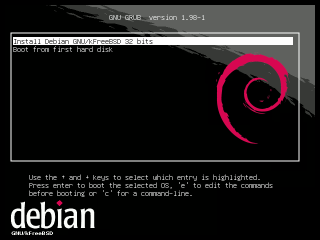
\includegraphics{image201008/kfreebsd-installer.png}
\caption{Debian GNU/kFreeBSDのDebianインストーラ}\label{debinstaller}
\end{center}
\end{figure}

インストール中の設定は以下を指定してインストールしました。

\begin{itemize}
 \item localeは「C」。(現時点のインストーラでは「C」と「English」のみの
localeしか指定できないため。)
 \item タイムゾーンはAsia/Japan。
 \item インストールは「Standard system utilities」(=Base System)のみ。
\end{itemize}

\subsection{初回起動}
\subsubsection{前準備}
X Window Systemをインストールしていないため、再起動後はコンソール環境で
起動します。
起動時にDHCPクライアントが起動するため、有線LAN環境であればIPアドレスを自動で
取得してネットワークにつながります。(以前は手動でdhclientを起動しないと
つながらなかった。)

カーネル起動後にインストーラで作成したユーザでログインし、最低限必要な以下の
パッケージをインストールし設定します。

\begin{commandline}
$ su
# apt-get update
# apt-get install sudo vim
# visudo
\end{commandline}

\subsubsection{カーネルの更新}

カーネルの起動メッセージを眺めているとCPUが1つしか認識していないように見えます。
現在起動中のカーネルとCPUの認識数を確認するとやはり1つしか認識していません。

\begin{commandline}
$ uname -a

GNU/kFreeBSD deb-NorTP60 7.3-1-686 #0
Tue Jul 20 02:12:21 CEST 2010 i686 i386
Genuine Intel(R) CPU           T2400  @ 1.83GHz GNU/kFreeBSD
\end{commandline}

\begin{commandline}
$ cat /proc/cpuinfo

processor   : 0
vendor_id   : GenuineIntel
cpu family  : 6
model       : 7
model name  : Genuine Intel(R) CPU           T2400  @ 1.83GHz
stepping    : 8
flags       : fpu vme de pse tsc msr pae mce cx8 apic sep mtrr pge mca
              cmov pat b19 b21 mmxext mmx fxsr xmm b26 b27 b28 b29 3dnow
cpu MHz     : 1828.76
bogomips    : 1828.76
\end{commandline}

現在利用できるカーネルを検索すると以下の候補が出てきます。

\begin{commandline}
$ apt-cache search kfreebsd-image-*

kfreebsd-headers-7.3-1-486 - header files for kernel of FreeBSD 7.3
kfreebsd-headers-7.3-1-686-smp - header files for kernel of FreeBSD 7.3
kfreebsd-headers-7.3-1-686 - header files for kernel of FreeBSD 7.3
kfreebsd-image-7-486 - kernel of FreeBSD 7 image
kfreebsd-image-7-686-smp - kernel of FreeBSD 7 image
kfreebsd-image-7-686 - kernel of FreeBSD 7 image
kfreebsd-image-7.3-1-486 - kernel of FreeBSD 7.3 image
kfreebsd-image-7.3-1-686-smp - kernel of FreeBSD 7.3 image
kfreebsd-image-7.3-1-686 - kernel of FreeBSD 7.3 image
kfreebsd-headers-8.0-1-486 - header files for kernel of FreeBSD 8.0
kfreebsd-headers-8.0-1-686-smp - header files for kernel of FreeBSD 8.0
kfreebsd-headers-8.0-1-686 - header files for kernel of FreeBSD 8.0
kfreebsd-image-8-486 - kernel of FreeBSD 8 image
kfreebsd-image-8-686-smp - kernel of FreeBSD 8 image
kfreebsd-image-8-686 - kernel of FreeBSD 8 image
kfreebsd-image-8.0-1-486 - kernel of FreeBSD 8.0 image
kfreebsd-image-8.0-1-686-smp - kernel of FreeBSD 8.0 image
kfreebsd-image-8.0-1-686 - kernel of FreeBSD 8.0 
\end{commandline}

シングルプロセッサ用とマルチプロセッサ用のカーネルは別々のようですので
マルチプロセッサ用カーネルをインストールし、再起動します。
\footnote{HyperThreadingのセキュリティ上の脆弱性に対応するためFreeBSD本家が
リリースするカーネルはHyperThreadingがデフォルトでOFFになっています。
Debian GNU/kFreeBSDでデフォルトがOFFであるかは対応CPUを持っていないため
確認できていません。}

カーネルのインストール処理でgrub2もアップデートされます。
\footnote{kfreebsd-image-8.0-1-686-smpをインストールしてみましたが、
インストール後に/へパーティションをマウントする処理に失敗し
起動できませんでした。FreeBSD 8.0 Release Noteに「''dangerously dedicated'' mode for the UFS file system is no longer supported. Important: Such disks will need to be reformatted to work with this release.」
という記述があるため、7.3から8.0へのカーネルアップグレードは
少し難しいようです。}

\begin{commandline}
$ sudo apt-get install kfreebsd-image-7.3-1-686-smp
$ sudo reboot
\end{commandline}

再起動し、カーネルとCPUの認識数を確認します。

\begin{commandline}
$ uname -a

GNU/kFreeBSD deb-NorTP60 7.3-1-686-smp #0
Tue Jul 20 02:43:20 CEST 2010 i686 i386
Genuine Intel(R) CPU           T2400  @ 1.83GHz GNU/kFreeBSD
\end{commandline}

\begin{commandline}
$ cat /proc/cpuinfo

processor   : 0
vendor_id   : GenuineIntel
cpu family  : 6
model       : 7
model name  : Genuine Intel(R) CPU           T2400  @ 1.83GHz
stepping    : 8
processor   : 1
vendor_id   : GenuineIntel
cpu family  : 6
model       : 7
model name  : Genuine Intel(R) CPU           T2400  @ 1.83GHz
stepping    : 8
flags       : fpu vme de pse tsc msr pae mce cx8 apic sep mtrr pge mca
              cmov pat b19 b21 mmxext mmx fxsr xmm b26 b27 b28 b29 3dnow
cpu MHz     : 1828.76
bogomips    : 1828.76
\end{commandline}

\subsection{Xorgのインストール}
X Window System環境が日常を過ごすため、xorgをインストールします。
しかしパッケージのインストール処理で以下のエラーが発生し、途中でインストールが
停止しました。

\begin{commandline}
$ sudo apt-get install xorg
Setting up hal (0.5.14-3) ...
Reloading system message bus config...
Failed to open connection to "system" message bus:
Failed to connect to socket /var/run/dbus/system_bus_socket: Connection refused
invoke-rc.d: initscript dbus, action "force-reload" failed.
Starting Hardware abstraction layer: haldinvoke-rc.d: initscript hal,
action "start" failed.
dpkg: error processing hal (--configure):
 subprocess installed post-installation script returned error exit status 1
\end{commandline}

\subsubsection{対応}

上記はhalのインストールの後処理でdbusの設定を再読み込みしようとしてエラーが
発生したため、パッケージのインストールが停止しました。
\footnote{\url{http://bugs.debian.org/cgi-bin/bugreport.cgi?bug=469528}}

psコマンドでdbusプロセスがいるか確認すると存在しません。
バグ修正はまだ行われていないため、とりあえずの措置として
「{\$} sudo /etc/init.d/dbus start」を実行してdbusを起動し
再度「{\$} sudo apt-get install xorg」を試みると次は以下のエラーに
変わりました。

\begin{commandline}
$ sudo /etc/init.d/dbus start
$ sudo apt-get install xorg
Setting up xserver-xorg (1:7.5+6) ...
invoke-rc.d: initscript hal, action "restart" failed.
dpkg: error processing xserver-xorg (--configure):
subprocess installed post-installation script returned error exit status 1
\end{commandline}

今度はxserver-xorgのインストールの後処理でhalと同様のエラーが発生したため、
再度halと同様に以下コマンドを実行し、xorgのインストールは完了しました。

\begin{commandline}
$ sudo /etc/init.d/dbus start
$ sudo apt-get install xorg
\end{commandline}

\subsubsection{X Window System起動及び設定}

この状態でstartxコマンドを実行するとX Window Systemの起動に成功しました。
しかし「/etc/X11/xorg.conf」の設定を確認しようとするとファイル自体が
存在しないためxorg.confを手動で作成します。

\begin{commandline}
$ sudo X -config
$ sudo cp xorg.conf.new /etc/X11/xorg.conf
\end{commandline}

再度startxを実行し、作成したxorg.confを用いてX Window Systemの起動が
確認できました。「/var/log/Xorg.0.log」を確認し'(EE)'の部分はないため、
動作は正常です。

\subsubsection{gdmのインストール(断念)}

ログイン画面もGUIで行いたいのでgdmをインストールします。

\begin{commandline}
$ sudo apt-get install gdm
\end{commandline}

gdmをインストールしrebootせずにgdmコマンドを実行するとマウス、キーボードは
問題なく動作します。

reboot後、自動でgdmが起動するのですがgdmのログイン画面でマウスは動きますが
キーボードが動作しません。(USBキーボードも動作しなかった。)

不本意ながらgdmによるログインは諦めstartxによる X Window Systemの起動に
切り替えることにしました。しかしこの状態ではカーネルの起動直後にgdmが
勝手に起動しキーボード入力ができなくなるため仮想コンソールに切り替えることも
できす、gdmをpurgeできません。

そのため、一度電源スイッチを長押ししてPCを停止、再起動してgdmが起動する前に
「Ctrl + Alt + F1」を連打してなんとか仮想コンソールに入り以下を実行してgdmを
purgeしました。

\begin{commandline}
$ sudo apt-get purge gdm
\end{commandline}

\subsection{デスクトップ環境の構築}

統合デスクトップ環境である「Xfce4」をインストールし、startxでXfce4を
起動するように.xinitrcを記述します。
.xinitrcは実行権が必要なため、実行権を付与します。

\begin{commandline}
$ sudo apt-get xfce4 xfce4-goodies
$ vim ~/.xinitrc
exec xfce4-session

$ chmod 744 ~/.xinitrc
$ startx
\end{commandline}

\subsection{日本語環境}

\subsubsection{日本語の表示}

日本語フォントをインストールします。

\begin{commandline}
$ sudo apt-get otf-ipafont otf-ipaexfont
\end{commandline}

日本語環境の「ja\_JP.UTF-8」ロケールはインストールされていなかったため
追加インストールします。

\begin{commandline}
$ sudo apt-get locales-all
\end{commandline}

startxコマンドでX Window Systemを起動するためlocaleの設定を.xinitrcに追記します。
Xfce4を終了して再度startxコマンドを実行するとXfce4が日本語環境で起動します。

\begin{commandline}
$ vim ~/.xinitrc    

export LANGUAGE='ja_JP.UTF-8'
export LC_ALL='ja_JP.UTF-8'
export LANG='ja_JP.UTF-8'
exec xfce4-session

$ startx
\end{commandline}

\subsubsection{日本語入力}

日本語入力環境としてuimを使用したいため、uimのインストールと設定をします。

\begin{commandline}
$ sudo apt-get install uim uim-anthy
$ vim ~/.xinitrc

export LANGUAGE='ja_JP.UTF-8'
export LC_ALL='ja_JP.UTF-8'
export LANG='ja_JP.UTF-8'

export XMODIFIRES='@im=uim'
export GTK_IM_MODULE='uim'
export QT_IM_MODULE='uim'

exec xfce4-session

$ startx
\end{commandline}

\subsection{開発環境のインストール}

Debian GNU/kFreeBSDのデバッグに必要なコンパイラ、パッケージの作成ツールを
インストールします。

\begin{commandline}
$ sudo apt-get update
$ sudo apt-get install gcc g++ gdb make
$ sudo apt-get install build-essential pbuilder debian-keyring
\end{commandline}

debパッケージのビルドができるかtcshをビルドして確認します。

\begin{commandline}
$ apt-get source tcsh
$ sudo apt-get build-dep tcsh
$ cd tcsh-6.17.00
$ dch
$ debuild -i -us -uc -b
$ sudo dpkg -i tcsh_6.17.00-3.1_kfreebsd-i386.deb
\end{commandline}

\subsection{Debian勉強会資料のビルド環境}

Debian勉強会での原稿はtexを採用しているため、原稿ファイルのビルド環境を
構築します。

texのビルドにはconrtib、non-freeのパッケージが必要なため、
apt-lineを修正します。

\begin{commandline}
$ sudo vim /etc/apt/sources.list
# deb http://ftp.jp.debian.org/debian/ squeeze main

deb http://ftp.jp.debian.org/debian/ squeeze main contrib non-free
deb-src http://ftp.jp.debian.org/debian/ squeeze main contrib non-free

deb http://security.debian.org/ squeeze/updates main
deb-src http://security.debian.org/ squeeze/updates main
\end{commandline}

必要なパッケージをインストールします。

\begin{commandline}
$ sudo apt-get install git-core
$ sudo apt-get install gs gs-esp gs-cjk-resource
$ sudo apt-get install ptex-bin xdvik-ja dvipsk-ja
$ sudo apt-get install okumura-clsfiles vfdata-morisawa5
$ sudo apt-get install texlive-latex-extra
$ sudo apt-get install poppler-data
$ sudo apt-get install evince
\end{commandline}

資料をダウンロードし、ビルドします。

\begin{commandline}
$ cd
$ git clone git://git.debian.org/git/tokyodebian/monthly-report.git/
$ cd monthly-report
$ make
\end{commandline}

\subsection{その他の日常環境の構築}

その他のよく使うソフトをインストールします。

\begin{commandline}
$ sudo apt-get install emacs emacs23-el
$ sudo apt-get install sylpheed sylpheed-i18n
$ sudo apt-get install iceweasel iceweasel-l10n-ja
$ sudo apt-get install audacious audacity
$ sudo apt-get install gxine
$ sudo apt-get install jd
$ sudo apt-get install gftp
\end{commandline}

\subsection{デバイスドライバ}
audaciousは音楽再生ソフトなのですが、実行しても音が鳴りません。
サウンドドライバをロードしているか確認するため「kldstat」を実行します。
\footnote{FreeBSDカーネルで読み込み中のカーネルモジュールの一覧を出力する
コマンドはkldstatですが、Debian GNU/KFreeBSDではlsmodがkldstatのリンクに
なっているためlsmodでも一覧を出力できます。}

\begin{commandline}
$ kldstat
 1   10 0xc0400000 890000   kfreebsd-7.3-1-686-smp.gz
 2    1 0xc0d9c000 57fdc    acpi.ko
 3    1 0xc5c7a000 67000    radeon.ko
 4    1 0xc5ce1000 14000    drm.ko
\end{commandline}

サウンドドライバがロードされていないためロードします。
\footnote{snd\_hdaはIntel945チップセットで音を鳴らすために必要な
サウンドドライバです。異なるサウンドチップを利用している場合は
環境に合わせてロードしてください。}

\begin{commandline}
$ sudo kldload snd_hda
$ kldstat
 1   10 0xc0400000 890000   kfreebsd-7.3-1-686-smp.gz
 2    1 0xc0d9c000 57fdc    acpi.ko
 3    1 0xc5c7a000 67000    radeon.ko
 4    1 0xc5ce1000 14000    drm.ko
 5    1 0xc611f000 1a000    snd_hda.ko
 6    1 0xc6139000 40000    sound.ko
\end{commandline}

音が鳴ることは確認できましたが、再起動するとサウンドドライバが読み込まれて
いない状態になります。そのため「/etc/modules」ファイルにカーネル起動時に
自動で読み込むドライバを設定します。
\footnote{Debian GNU/kFreeBSDに/sbin/modprobeコマンドはあるのですが
/sbin/kldloadのリンクになっているため、modprobeをしただけで再起動後も
自動でモジュールを読み込むようにはなっていないようです。}

\begin{commandline}
$ sudo vim /etc/modules
# /etc/modules: kernel modules to load at boot time.
#
# This file should contain the names of kernel modules that are
# to be loaded at boot time, one per line.  Comments begin with
# a ``#'', and everything on the line after them is ignored.
snd_hda.ko
\end{commandline}

\subsection{今後の課題}
Debian GNU/kFreeBSDでセットアップ作業を行いましたが日常生活を送るに向けて
いくつか課題が残っています。

\begin{itemize}
 \item WebブラウザでのFlashの再生(Adobe公式のFlashバイナリにFreeBSD版は
まだない)
 \item ビデオ再生(映像が乱れる。おそらくcodecの問題)
\end{itemize}

今後にむけた取り組みとして以下を試していきたいです。

\begin{itemize}
 \item Linuxバイナリ互換機能
 \item 仮想化機能(Jail、VirtualBox、qemu)
 \item ZFS
\end{itemize}

\subsection{環境構築を終えて}
インストーラの整備も進んでおり、X Window Systemの導入後はDebian GNU/Linuxと
なんら変わらない手順で環境構築ができました。

ただ問題が発生したときにFreeBSDカーネルとDebianの両方の知識が必要なため、
原因を調べるのが大変でFreeBSDとDebianの両方の情報源に当たってなんとか
解決しました。

バグ報告があると同じところでつまずいている人と情報を共有できるので
できるだけバグ報告は上げましょう。

Debian GNU/kFreeBSDは品質も徐々に上がってきており、Squeezeで技術プレビュー
扱いのリリースがされる予定です。\footnote{\url{http://www.debian.org/News/2010/20100806}}
みなさんもぜひDebian GNU/kFreeBSDをデバッグしてSqueezeリリースまでに品質を
高めましょう。

\subsection{参考資料}
\begin{itemize}
 \item 東京エリア Debian 出張勉強会 発表スライド(岩松信洋) : \url{http://tokyodebian.alioth.debian.org/pdf/debianmeetingresume201006-iwamatsu-presentation.pdf}
 \item Debian wiki : \url{http://wiki.debian.org/Debian\_GNU/kFreeBSD\_FAQ}
\end{itemize}

%debianmeetingresume201011.tex
%-------------------------------------------------------------------------------
\dancersection{Debian Miniconf 計画検討}{山本 浩之}
%-------------------------------------------------------------------------------
\index{miniconf}

毎月恒例になるらしい、ブレストタイム。
Debian Miniconf in Japan に向けてみんなでブレストします。

\subsection{先月までに決まっていること}
\subsubsection{聴衆のメインターゲット}
Debian だけに限らない開発者やユーザ。アップストリーム開発者や翻訳者も含む。ビジネス関係の人たちは二の次。

\subsubsection{開催形態}
日本で開催される FLOSS 関係の国際会議に相乗りして開催。勿論、基本的に英語で。

\subsubsection{現在までに出ているネタ}
\begin{itemize}
 \item Embedded セッション\\
       組込における Debian の取り組み。
 \item ライセンスセッション\\
       ソフトウェア作成者とコンテンツ作成者とのフリーなライセンスでの交流。
 \item 事例集セッション\\
       Debianを導入した企業や団体の事例を通じ、なぜDebianなのかを語る。
 \item プログラム言語系セッション\\
特に Ruby や関数言語系における Debian の取り組み。
 \item VPS・クラウドセッション\\
Debian における VPS ・クラウドに関するパッケージや開発状況。
 \item WEB アプリケーションセッション\\
Debian における WEB アプリケーションに関するパッケージや開発状況。
 \item Debian からの派生ディストリビューションセッション\\
数多くあるDebian からの派生ディストリビューションとの、お互いの交流や要求。
 \item ハックラボ\\
圧倒的人気により、当確(?)。
\end{itemize}

%debianmeetingresume201007.tex
%資料無し

%debianmeetingresume201008.tex
%資料無し

%debianmeetingresume201009.tex
%OSC 2010 Tokyo/Fallのため資料無し

%debianmeetingresume201010.tex
%\dancersection{OSC北海道参加報告}{荒木靖宏}
%-------------------------------------------------------------------------------
%\index{OSC-Do 2010}
%
%
%荒木の発表は「あなたはどっち、CloudでDebian, DebianでCloud」という題でDebianでのCloudにまつわる話をしました。
%
%岩松の発表は「squeezeに向けたDebian GNU/kFreeBSD入門」という題でDebian GNU/kFreeBSDがどのようにDebianにはいり、どのように使用するのか、などの話をしました。
%
%土曜日の朝最初のセッションで出足を心配したのですが、割り当てられた部屋はほぼ満員でした。
%
%また、GPGキーサインパーティには事前に6人の参加表明があり、飛び入りもあり、合計8名でした。
%

%201011 kansai KOF 2010のためtex資料無し
%debianmeetingresume201011-kansai-presentation.rbt
%Fix me. CUTとnon-upload Developerの紹介を抜粋するか?

% FIXME: quizを追加すること
% 今回はquiz無し

\printindex

% add page to even number
%\newpage
%\thispagestyle{empty}\mbox{}

\newpage
\thispagestyle{empty}\mbox{}
\newpage

\thispagestyle{empty} 
{
\large
\begin{itembox}{\bf 『あんどきゅめんてっど でびあん』について}
本書は、東京および関西周辺で毎月行なわれている『東京エリア Debian 勉強会』および
『関西エリア Debian 勉強会』で
使用された資料・小ネタ・必殺技などを一冊にまとめたものです。
収録範囲は東京エリアは2010年6月勉強会(第65回)から2010年11月勉強会(第70回)、関西エリアは第36回から第41回 まで。
% FIXME: 回数を修正すること。
内容は無保証、つっこみなどがあれば勉強会にて。
\end{itembox}
}

\vspace*{15cm}
{\color{dancerlightblue}\rule{\hsize}{1mm}}
\vspace{2mm}

\includegraphics[width=2cm]{image200502/openlogo-nd.eps}
\noindent \Large \bf あんどきゅめんてっど でびあん 2010年冬号\\
\noindent \normalfont 2010年12月31日 \hspace{5mm}  初版第1刷発行\\
\noindent \normalfont 東京エリア Debian 勉強会/関西エリア Debian 勉強会 (編集・印刷・発行)\\
{\color{dancerdarkblue}\rule{\hsize}{1mm}}

\end{document}
